% \newcommand{\Draftmode}{\True}

%========================================Statement=============================%
% The following is the statement about this slide:
%   (1) This slide is based on the template of beamer with style
%       Cambridge US. All of the copyright belong to them.
%   (2) This slide is used to introduce the fundamental papers &
%       project for class CS7485 in CCIS at NE.
%==============================================================================%
\documentclass[aspectratio=169]{beamer}
\usetheme{default}%Singapore}%Pittsburgh}%Szeged}
\usecolortheme{default}
\setbeamercovered{dynamic}
\setbeamertemplate{navigation symbols}{}
\usepackage{helvet}
\usefonttheme{structurebold}
% \setbeamertemplate{footline}[frame number]{}
\setbeamertemplate{footline}{%
  \raisebox{5pt}{\makebox[\paperwidth]{\hfill\makebox[10pt]{\scriptsize\textcolor{gray}{\insertframenumber\qquad}}}}}

\usepackage{ragged2e}
\apptocmd{\frame}{\justifying}{}{}
%================================Customize Colors==============================%
\definecolor{myblue}{rgb}{0.725, 0.796, 1.000}
\definecolor{mygreen}{rgb}{0.012, 0.612, 0.388}
\definecolor{mypurple}{rgb}{0.518, 0.00, 0.518}
%=================================Cover Page===================================%
\usepackage{lipsum}
\usepackage{enumerate}
\usepackage{bbm}
\usepackage{dsfont}
\usepackage{pdfpages}
\usepackage{multirow}
\usepackage{pgf}
\usepackage{makecell}
% *** MATH PACKAGES ***
\usepackage{amsmath}
\usepackage{amssymb}
\usepackage{amsthm}
\usepackage{pifont}

% *** ALIGNMENT PACKAGES ***
\usepackage{array}

% *** SUBFIGURE PACKAGES ***

% *** BOX PACKAGE ***
\usepackage{fancybox}

% *** PDF, URL AND HYPERLINK PACKAGES ***
\usepackage{url}

\usepackage{tikz}
\usetikzlibrary{arrows,chains,matrix,positioning,scopes,3d,automata,backgrounds,fit,shapes}
\usepackage{smartdiagram}
\usepackage{pgfplots}
\usetikzlibrary{plotmarks}

\usepackage[nodayofweek]{datetime}
\usepackage{rotating}

\usepackage[noend]{algorithmic}
\usepackage{algorithm}
\usepackage{syntax, etoolbox}
\renewcommand{\syntleft}{\normalfont\itshape}   % do not display '<' associated with variable, e.g., <A>
\renewcommand{\syntright}{}  % do not display '>' associated with variable, e.g., <A>

\usepackage{stmaryrd}
\usepackage{wasysym}
\usepackage{tabularx}
\usepackage{listings}
\lstset{frameround=fttt, 
  language=C++,
  keywordstyle=\color{blue}\ttfamily,
  stringstyle=\color{red}\ttfamily,
  commentstyle=\color{green}\ttfamily,
  morecomment=[l][\color{magenta}]{\#},
  escapechar=@,
  basicstyle=\fontsize{7}{8}\selectfont\ttfamily,
  emph={decl, begin, end, goto, start_thread,
    assume,assert,wait,broadcast,int,if,return,while},
  commentstyle=\color{mygreen}}

\newcommand{\localCommand}{} % command names start with \
\newlength {\localLength}    % length  names start with \
\newcounter {localCounter}   % counter names have  no \

\newcommand{\newlengthset}       [2]{\newlength {#1} \setlength {#1}{#2}}
\newcommand{\newlengthsettowidth}[2]{\newlength {#1} \settowidth{#1}{#2}}
\newcommand{\newcounterset}      [2]{\newcounter{#1} \setcounter{#1}{#2}}

\newcommand{\ensurecommand}[2]{
  \providecommand{#1}{}
  \renewcommand{#1}{#2}}

% Number ranges and other set symbols

\newcommand{\numberRange}[1]{\mathbb #1}
\newcommand{\NN}{\numberRange N}                             % naturals
\newcommand{\ZZ}{\numberRange Z}                             % integers
\newcommand{\QQ}{\numberRange Q}                             % rationals
\newcommand{\RR}{\numberRange R}                             % reals
\newcommand{\CC}{\numberRange C}                             % complexes
\newcommand{\BS}{\{0,1\}}                               % boolean space
\newcommand{\OO}{\mathcal O}                            % Landau

\newcommand{\PP}{\mathds P}                             % Program
\newcommand{\BB}{\mathds B}                             % boolean program
\newcommand{\range}[3][X]{\Ifthen{\Equal{#1}{X}}{\{}#2,\ldots,#3\Ifthen{\Equal{#1}{X}}{\}}} % {1,...,n}, or 1,...,n if no optional arg
\newcommand{\power}[1]{2^{#1}} % \mathcal P(#1)}        % power set

\newcommand{\complexity}[1]{\mbox{\bfseries #1}}
\newcommand{\PTIME} {\complexity{P}}
\newcommand{\NP}    {\complexity{NP}}
\newcommand{\PSPACE}{\complexity{PSPACE}}

% Relational symbols

\newcommand{\atl}{\geq}                                 % at least
\newcommand{\atm}{\leq}                                 % at most
%\newcommand{\divides} {\operatorname{|}}                % divides % use MnSymbol package
\newcommand{\st}  {\operatorname{|}}                    % such that: { x | f(x) = 10 }
\newcommand{\mmod}{\operatorname{mod}}                  % '\pmod' creates huge space before the 'mod'
\newcommand{\grammarOr}{\ \mbox{\Large $\mid$} \ }

\newcommand{\union}       {\mathbin        {\cup}}      % set union
\newcommand{\Union}       {\operatorname{\bigcup}}      % big union
\newcommand{\intersection}{\mathbin        {\cap}}      % set intersection
\newcommand{\Intersection}{\operatorname{\bigcap}}      % big intersection
                                                        % set complement is \complement
\newcommand{\argmin}{\operatorname{argmin}}
\newcommand{\argmax}{\operatorname{argmax}}

\newcommand{\superset}   {\supset}                      % superset ">"
\newcommand{\superseteq} {\supseteq}                    % superset ">="
\newcommand{\supersetneq}{\supsetneqq}                  % strict superset with emphasis (avoid)

% Calculus and algebra

\newcommand{\func}[3]{#1 \colon #2 \rightarrow #3}      % function f:A->B
\newcommand{\restr}[2]{#1\big|_{#2}}                    % function f restricted to X (f|X)
\newcommand{\deriv}[2]{#1^{(\mathit{#2})}}              % higher derivatives of a function
\newcommand{\dd}{\,d}                                   % differential symbol with preceding space
\newcommand{\mtrans}[1]{{#1}^{\mathbf{T}}}              % transpose of a matrix
\newcommand{\binCoeff}[2]{                              % binomial coefficient "#1 choose #2"
  \mbox{\scriptsize{$\left(\begin{array}{c} #1 \\ #2 \end{array} \right)$}}}
\newcommand{\flip}[2]{(#1 \ #2)}                        % transposition of two elements: (2 3)


% Parentheses, ceilings, floors and angle brackets - small and big

\newcommand{\parens}  [1]{        (    #1          )   } % argument in (.) (added for completeness)
\newcommand{\ceils}   [1]{     \lceil  #1       \rceil } % argument in ceilings
\newcommand{\floors}  [1]{     \lfloor #1       \rfloor} % argument in floors
\newcommand{\angles}  [1]{     \langle #1       \rangle} % argument in <.>
\newcommand{\brackets}[1]{        [    #1          ]   } % argument in [.]

\newcommand{\Parens}  [1]{\left(       #1 \right)      } % argument in big (.)
\newcommand{\Ceils}   [1]{\left\lceil  #1 \right\rceil}  % argument in big ceilings
\newcommand{\Floors}  [1]{\left\lfloor #1 \right\rfloor} % argument in big floors
\newcommand{\Angles}  [1]{\left\langle #1 \right\rangle} % argument in big <.>
\newcommand{\Brackets}[1]{\left   [    #1 \right   ]   } % argument in big [.]


% Boolean connectives. These already exist: \land, \lor, \lnot

\newcommand{\limplies}{\Rightarrow}               % logical 'implies'
\newcommand{\lfollows}{\Leftarrow}                % logical 'follows from' (converse of implies)
\newcommand{\lequiv}  {\Leftrightarrow}           % logical 'equivalent'. Also \equiv
\newcommand{\lxor}    {\oplus}                    % logical 'exclusive or'
\newcommand{\lexor}   {\oplus}                    % ditto
\newcommand{\bigland} {\bigwedge}
\newcommand{\biglor}  {\bigvee}
\newcommand{\false}   {\mathit{false}}
\newcommand{\true}    {\mathit{true}}

\newcommand{\Hoare}[3]{\angles{#1} \ \mbox{\code{#2}} \ \angles{#3}}  % Hoare triple: <#1> #2 <#3>. Use: \Hoare{x > 10}{$x$++}{x > 10}

% Conditional compilation
% I found out on Mar 10, 2007 that if-then-else cannot be nested within the condition:
% \ifthenelse {\ifthenelse{\equal{1}{1}}{\equal{1}{1}}{\equal{1}{2}}} {Yes} {No} % gives Tex error
% Nesting within the then-branch and the else-branch seems ok

\newcommand{\Ifthenelse}[3]{\ifthenelse{#1}{#2}{#3}}   % for consistency: initial capital
\newcommand{\Ifthen}    [2]{\Ifthenelse{#1}{#2}{}}
\newcommand{\Unless}    [2]{\Ifthen{\not {#1}}{#2}}
\newcommand{\Equal}     [2]{\equal{#1}{#2}}            % for consistency: initial capital
\newcommand{\Empty}     [1]{\Equal{#1}{}}
\newcommand{\True}         {\Equal{1}{1}}
\newcommand{\False}        {\Equal{1}{2}}



% Enumeration with specific counter types. Usage:
% \begin{enumerate} \alphaenumi
%
% \item ...

\newcommand{\renewcounter}[4]{\renewcommand{#1}{(#4 {#3})}\renewcommand{#2}{(#4 {#3})}}

\newcommand{\alphaenumi}{\renewcounter{\theenumi}{\labelenumi}{enumi}{\alph}}  % (a) ... (e)
\newcommand{\Alphaenumi}{\renewcounter{\theenumi}{\labelenumi}{enumi}{\Alph}}  % (A) ... (E)
\newcommand{\romanenumi}{\renewcounter{\theenumi}{\labelenumi}{enumi}{\roman}} % (i) ... (v)
\newcommand{\Romanenumi}{\renewcounter{\theenumi}{\labelenumi}{enumi}{\Roman}} % (I) ... (V)

\newcommand{\alphaenumii}{\renewcounter{\theenumii}{\labelenumii}{enumii}{\alph}}
\newcommand{\Alphaenumii}{\renewcounter{\theenumii}{\labelenumii}{enumii}{\Alph}}
\newcommand{\romanenumii}{\renewcounter{\theenumii}{\labelenumii}{enumii}{\roman}}
\newcommand{\Romanenumii}{\renewcounter{\theenumii}{\labelenumii}{enumii}{\Roman}}


% Draft. I don't use latex's [draft] option because it needlessly suppresses graphics includes.
% Use the following header structure:

% % Begin Customization Section. Comment these out to turn the flag off.
%
%\newcommand{\Draftmode}{\True}
%\newcommand{\SomeFlag} {\True}
%
% % End Customization Section
%
% % Default values of options:
%
%\providecommand{\SomeFlag}{\False}
%
%\documentclass{...}
%
%\newcommand{\localCommand}{} % command names start with \
\newlength {\localLength}    % length  names start with \
\newcounter {localCounter}   % counter names have  no \

\newcommand{\newlengthset}       [2]{\newlength {#1} \setlength {#1}{#2}}
\newcommand{\newlengthsettowidth}[2]{\newlength {#1} \settowidth{#1}{#2}}
\newcommand{\newcounterset}      [2]{\newcounter{#1} \setcounter{#1}{#2}}

\newcommand{\ensurecommand}[2]{
  \providecommand{#1}{}
  \renewcommand{#1}{#2}}

% Number ranges and other set symbols

\newcommand{\numberRange}[1]{\mathbb #1}
\newcommand{\NN}{\numberRange N}                             % naturals
\newcommand{\ZZ}{\numberRange Z}                             % integers
\newcommand{\QQ}{\numberRange Q}                             % rationals
\newcommand{\RR}{\numberRange R}                             % reals
\newcommand{\CC}{\numberRange C}                             % complexes
\newcommand{\BS}{\{0,1\}}                               % boolean space
\newcommand{\OO}{\mathcal O}                            % Landau

\newcommand{\PP}{\mathds P}                             % Program
\newcommand{\BB}{\mathds B}                             % boolean program
\newcommand{\range}[3][X]{\Ifthen{\Equal{#1}{X}}{\{}#2,\ldots,#3\Ifthen{\Equal{#1}{X}}{\}}} % {1,...,n}, or 1,...,n if no optional arg
\newcommand{\power}[1]{2^{#1}} % \mathcal P(#1)}        % power set

\newcommand{\complexity}[1]{\mbox{\bfseries #1}}
\newcommand{\PTIME} {\complexity{P}}
\newcommand{\NP}    {\complexity{NP}}
\newcommand{\PSPACE}{\complexity{PSPACE}}

% Relational symbols

\newcommand{\atl}{\geq}                                 % at least
\newcommand{\atm}{\leq}                                 % at most
%\newcommand{\divides} {\operatorname{|}}                % divides % use MnSymbol package
\newcommand{\st}  {\operatorname{|}}                    % such that: { x | f(x) = 10 }
\newcommand{\mmod}{\operatorname{mod}}                  % '\pmod' creates huge space before the 'mod'
\newcommand{\grammarOr}{\ \mbox{\Large $\mid$} \ }

\newcommand{\union}       {\mathbin        {\cup}}      % set union
\newcommand{\Union}       {\operatorname{\bigcup}}      % big union
\newcommand{\intersection}{\mathbin        {\cap}}      % set intersection
\newcommand{\Intersection}{\operatorname{\bigcap}}      % big intersection
                                                        % set complement is \complement
\newcommand{\argmin}{\operatorname{argmin}}
\newcommand{\argmax}{\operatorname{argmax}}

\newcommand{\superset}   {\supset}                      % superset ">"
\newcommand{\superseteq} {\supseteq}                    % superset ">="
\newcommand{\supersetneq}{\supsetneqq}                  % strict superset with emphasis (avoid)

% Calculus and algebra

\newcommand{\func}[3]{#1 \colon #2 \rightarrow #3}      % function f:A->B
\newcommand{\restr}[2]{#1\big|_{#2}}                    % function f restricted to X (f|X)
\newcommand{\deriv}[2]{#1^{(\mathit{#2})}}              % higher derivatives of a function
\newcommand{\dd}{\,d}                                   % differential symbol with preceding space
\newcommand{\mtrans}[1]{{#1}^{\mathbf{T}}}              % transpose of a matrix
\newcommand{\binCoeff}[2]{                              % binomial coefficient "#1 choose #2"
  \mbox{\scriptsize{$\left(\begin{array}{c} #1 \\ #2 \end{array} \right)$}}}
\newcommand{\flip}[2]{(#1 \ #2)}                        % transposition of two elements: (2 3)


% Parentheses, ceilings, floors and angle brackets - small and big

\newcommand{\parens}  [1]{        (    #1          )   } % argument in (.) (added for completeness)
\newcommand{\ceils}   [1]{     \lceil  #1       \rceil } % argument in ceilings
\newcommand{\floors}  [1]{     \lfloor #1       \rfloor} % argument in floors
\newcommand{\angles}  [1]{     \langle #1       \rangle} % argument in <.>
\newcommand{\brackets}[1]{        [    #1          ]   } % argument in [.]

\newcommand{\Parens}  [1]{\left(       #1 \right)      } % argument in big (.)
\newcommand{\Ceils}   [1]{\left\lceil  #1 \right\rceil}  % argument in big ceilings
\newcommand{\Floors}  [1]{\left\lfloor #1 \right\rfloor} % argument in big floors
\newcommand{\Angles}  [1]{\left\langle #1 \right\rangle} % argument in big <.>
\newcommand{\Brackets}[1]{\left   [    #1 \right   ]   } % argument in big [.]


% Boolean connectives. These already exist: \land, \lor, \lnot

\newcommand{\limplies}{\Rightarrow}               % logical 'implies'
\newcommand{\lfollows}{\Leftarrow}                % logical 'follows from' (converse of implies)
\newcommand{\lequiv}  {\Leftrightarrow}           % logical 'equivalent'. Also \equiv
\newcommand{\lxor}    {\oplus}                    % logical 'exclusive or'
\newcommand{\lexor}   {\oplus}                    % ditto
\newcommand{\bigland} {\bigwedge}
\newcommand{\biglor}  {\bigvee}
\newcommand{\false}   {\mathit{false}}
\newcommand{\true}    {\mathit{true}}

\newcommand{\Hoare}[3]{\angles{#1} \ \mbox{\code{#2}} \ \angles{#3}}  % Hoare triple: <#1> #2 <#3>. Use: \Hoare{x > 10}{$x$++}{x > 10}

% Conditional compilation
% I found out on Mar 10, 2007 that if-then-else cannot be nested within the condition:
% \ifthenelse {\ifthenelse{\equal{1}{1}}{\equal{1}{1}}{\equal{1}{2}}} {Yes} {No} % gives Tex error
% Nesting within the then-branch and the else-branch seems ok

\newcommand{\Ifthenelse}[3]{\ifthenelse{#1}{#2}{#3}}   % for consistency: initial capital
\newcommand{\Ifthen}    [2]{\Ifthenelse{#1}{#2}{}}
\newcommand{\Unless}    [2]{\Ifthen{\not {#1}}{#2}}
\newcommand{\Equal}     [2]{\equal{#1}{#2}}            % for consistency: initial capital
\newcommand{\Empty}     [1]{\Equal{#1}{}}
\newcommand{\True}         {\Equal{1}{1}}
\newcommand{\False}        {\Equal{1}{2}}



% Enumeration with specific counter types. Usage:
% \begin{enumerate} \alphaenumi
%
% \item ...

\newcommand{\renewcounter}[4]{\renewcommand{#1}{(#4 {#3})}\renewcommand{#2}{(#4 {#3})}}

\newcommand{\alphaenumi}{\renewcounter{\theenumi}{\labelenumi}{enumi}{\alph}}  % (a) ... (e)
\newcommand{\Alphaenumi}{\renewcounter{\theenumi}{\labelenumi}{enumi}{\Alph}}  % (A) ... (E)
\newcommand{\romanenumi}{\renewcounter{\theenumi}{\labelenumi}{enumi}{\roman}} % (i) ... (v)
\newcommand{\Romanenumi}{\renewcounter{\theenumi}{\labelenumi}{enumi}{\Roman}} % (I) ... (V)

\newcommand{\alphaenumii}{\renewcounter{\theenumii}{\labelenumii}{enumii}{\alph}}
\newcommand{\Alphaenumii}{\renewcounter{\theenumii}{\labelenumii}{enumii}{\Alph}}
\newcommand{\romanenumii}{\renewcounter{\theenumii}{\labelenumii}{enumii}{\roman}}
\newcommand{\Romanenumii}{\renewcounter{\theenumii}{\labelenumii}{enumii}{\Roman}}


% Draft. I don't use latex's [draft] option because it needlessly suppresses graphics includes.
% Use the following header structure:

% % Begin Customization Section. Comment these out to turn the flag off.
%
%\newcommand{\Draftmode}{\True}
%\newcommand{\SomeFlag} {\True}
%
% % End Customization Section
%
% % Default values of options:
%
%\providecommand{\SomeFlag}{\False}
%
%\documentclass{...}
%
%\newcommand{\localCommand}{} % command names start with \
\newlength {\localLength}    % length  names start with \
\newcounter {localCounter}   % counter names have  no \

\newcommand{\newlengthset}       [2]{\newlength {#1} \setlength {#1}{#2}}
\newcommand{\newlengthsettowidth}[2]{\newlength {#1} \settowidth{#1}{#2}}
\newcommand{\newcounterset}      [2]{\newcounter{#1} \setcounter{#1}{#2}}

\newcommand{\ensurecommand}[2]{
  \providecommand{#1}{}
  \renewcommand{#1}{#2}}

% Number ranges and other set symbols

\newcommand{\numberRange}[1]{\mathbb #1}
\newcommand{\NN}{\numberRange N}                             % naturals
\newcommand{\ZZ}{\numberRange Z}                             % integers
\newcommand{\QQ}{\numberRange Q}                             % rationals
\newcommand{\RR}{\numberRange R}                             % reals
\newcommand{\CC}{\numberRange C}                             % complexes
\newcommand{\BS}{\{0,1\}}                               % boolean space
\newcommand{\OO}{\mathcal O}                            % Landau

\newcommand{\PP}{\mathds P}                             % Program
\newcommand{\BB}{\mathds B}                             % boolean program
\newcommand{\range}[3][X]{\Ifthen{\Equal{#1}{X}}{\{}#2,\ldots,#3\Ifthen{\Equal{#1}{X}}{\}}} % {1,...,n}, or 1,...,n if no optional arg
\newcommand{\power}[1]{2^{#1}} % \mathcal P(#1)}        % power set

\newcommand{\complexity}[1]{\mbox{\bfseries #1}}
\newcommand{\PTIME} {\complexity{P}}
\newcommand{\NP}    {\complexity{NP}}
\newcommand{\PSPACE}{\complexity{PSPACE}}

% Relational symbols

\newcommand{\atl}{\geq}                                 % at least
\newcommand{\atm}{\leq}                                 % at most
%\newcommand{\divides} {\operatorname{|}}                % divides % use MnSymbol package
\newcommand{\st}  {\operatorname{|}}                    % such that: { x | f(x) = 10 }
\newcommand{\mmod}{\operatorname{mod}}                  % '\pmod' creates huge space before the 'mod'
\newcommand{\grammarOr}{\ \mbox{\Large $\mid$} \ }

\newcommand{\union}       {\mathbin        {\cup}}      % set union
\newcommand{\Union}       {\operatorname{\bigcup}}      % big union
\newcommand{\intersection}{\mathbin        {\cap}}      % set intersection
\newcommand{\Intersection}{\operatorname{\bigcap}}      % big intersection
                                                        % set complement is \complement
\newcommand{\argmin}{\operatorname{argmin}}
\newcommand{\argmax}{\operatorname{argmax}}

\newcommand{\superset}   {\supset}                      % superset ">"
\newcommand{\superseteq} {\supseteq}                    % superset ">="
\newcommand{\supersetneq}{\supsetneqq}                  % strict superset with emphasis (avoid)

% Calculus and algebra

\newcommand{\func}[3]{#1 \colon #2 \rightarrow #3}      % function f:A->B
\newcommand{\restr}[2]{#1\big|_{#2}}                    % function f restricted to X (f|X)
\newcommand{\deriv}[2]{#1^{(\mathit{#2})}}              % higher derivatives of a function
\newcommand{\dd}{\,d}                                   % differential symbol with preceding space
\newcommand{\mtrans}[1]{{#1}^{\mathbf{T}}}              % transpose of a matrix
\newcommand{\binCoeff}[2]{                              % binomial coefficient "#1 choose #2"
  \mbox{\scriptsize{$\left(\begin{array}{c} #1 \\ #2 \end{array} \right)$}}}
\newcommand{\flip}[2]{(#1 \ #2)}                        % transposition of two elements: (2 3)


% Parentheses, ceilings, floors and angle brackets - small and big

\newcommand{\parens}  [1]{        (    #1          )   } % argument in (.) (added for completeness)
\newcommand{\ceils}   [1]{     \lceil  #1       \rceil } % argument in ceilings
\newcommand{\floors}  [1]{     \lfloor #1       \rfloor} % argument in floors
\newcommand{\angles}  [1]{     \langle #1       \rangle} % argument in <.>
\newcommand{\brackets}[1]{        [    #1          ]   } % argument in [.]

\newcommand{\Parens}  [1]{\left(       #1 \right)      } % argument in big (.)
\newcommand{\Ceils}   [1]{\left\lceil  #1 \right\rceil}  % argument in big ceilings
\newcommand{\Floors}  [1]{\left\lfloor #1 \right\rfloor} % argument in big floors
\newcommand{\Angles}  [1]{\left\langle #1 \right\rangle} % argument in big <.>
\newcommand{\Brackets}[1]{\left   [    #1 \right   ]   } % argument in big [.]


% Boolean connectives. These already exist: \land, \lor, \lnot

\newcommand{\limplies}{\Rightarrow}               % logical 'implies'
\newcommand{\lfollows}{\Leftarrow}                % logical 'follows from' (converse of implies)
\newcommand{\lequiv}  {\Leftrightarrow}           % logical 'equivalent'. Also \equiv
\newcommand{\lxor}    {\oplus}                    % logical 'exclusive or'
\newcommand{\lexor}   {\oplus}                    % ditto
\newcommand{\bigland} {\bigwedge}
\newcommand{\biglor}  {\bigvee}
\newcommand{\false}   {\mathit{false}}
\newcommand{\true}    {\mathit{true}}

\newcommand{\Hoare}[3]{\angles{#1} \ \mbox{\code{#2}} \ \angles{#3}}  % Hoare triple: <#1> #2 <#3>. Use: \Hoare{x > 10}{$x$++}{x > 10}

% Conditional compilation
% I found out on Mar 10, 2007 that if-then-else cannot be nested within the condition:
% \ifthenelse {\ifthenelse{\equal{1}{1}}{\equal{1}{1}}{\equal{1}{2}}} {Yes} {No} % gives Tex error
% Nesting within the then-branch and the else-branch seems ok

\newcommand{\Ifthenelse}[3]{\ifthenelse{#1}{#2}{#3}}   % for consistency: initial capital
\newcommand{\Ifthen}    [2]{\Ifthenelse{#1}{#2}{}}
\newcommand{\Unless}    [2]{\Ifthen{\not {#1}}{#2}}
\newcommand{\Equal}     [2]{\equal{#1}{#2}}            % for consistency: initial capital
\newcommand{\Empty}     [1]{\Equal{#1}{}}
\newcommand{\True}         {\Equal{1}{1}}
\newcommand{\False}        {\Equal{1}{2}}



% Enumeration with specific counter types. Usage:
% \begin{enumerate} \alphaenumi
%
% \item ...

\newcommand{\renewcounter}[4]{\renewcommand{#1}{(#4 {#3})}\renewcommand{#2}{(#4 {#3})}}

\newcommand{\alphaenumi}{\renewcounter{\theenumi}{\labelenumi}{enumi}{\alph}}  % (a) ... (e)
\newcommand{\Alphaenumi}{\renewcounter{\theenumi}{\labelenumi}{enumi}{\Alph}}  % (A) ... (E)
\newcommand{\romanenumi}{\renewcounter{\theenumi}{\labelenumi}{enumi}{\roman}} % (i) ... (v)
\newcommand{\Romanenumi}{\renewcounter{\theenumi}{\labelenumi}{enumi}{\Roman}} % (I) ... (V)

\newcommand{\alphaenumii}{\renewcounter{\theenumii}{\labelenumii}{enumii}{\alph}}
\newcommand{\Alphaenumii}{\renewcounter{\theenumii}{\labelenumii}{enumii}{\Alph}}
\newcommand{\romanenumii}{\renewcounter{\theenumii}{\labelenumii}{enumii}{\roman}}
\newcommand{\Romanenumii}{\renewcounter{\theenumii}{\labelenumii}{enumii}{\Roman}}


% Draft. I don't use latex's [draft] option because it needlessly suppresses graphics includes.
% Use the following header structure:

% % Begin Customization Section. Comment these out to turn the flag off.
%
%\newcommand{\Draftmode}{\True}
%\newcommand{\SomeFlag} {\True}
%
% % End Customization Section
%
% % Default values of options:
%
%\providecommand{\SomeFlag}{\False}
%
%\documentclass{...}
%
%\input{general}

\providecommand{\Draftmode}{\False}

\newcommand{\draftcolor}{red}

\newcommand{\Itedraft}    [2]{\Ifthenelse{\Draftmode}{#1}{#2}}
\newcommand{\Ifdraft}     [1]{\Itedraft{#1}{}}
\newcommand{\Unlessdraft} [1]{\Itedraft{}{#1}}
\newcommand{\drafttext}   [2][\draftcolor]{\Ifdraft{{\color{#1}#2}}}
\newcommand{\draftpointer}{\makebox[0mm][c]{$^*$}}
\newcommand{\draftmargin} [2][\draftcolor]{\drafttext[#1]{\draftpointer\marginpar[\raggedleft\small{\color{#1}#2}]{\raggedright\small{\color{#1}#2}}}} % marginalia, shown in draftmode only
\newcommand{\draftdate}   [1][\today]{\drafttext{\makebox[0mm][l]{\normalfont\tiny \ \ (Draft of #1)}}} % use behind title or author names
\newcommand{\draftsection}[2][Draft Material]{\Ifdraft{           \section*{#1} #2}}  % this and the next don't work with the "letter" class (which doesn't have \section)
\newcommand{\Draftsection}[2][Draft Material]{\Ifdraft{\clearpage \section*{#1} #2}}
\newcommand{\draftnewpage}  {\Ifdraft{\newpage}}
\newcommand{\draftclearpage}{\Ifdraft{\clearpage}}

\newcommand{\draftauthor} [3]{
  \newcommand{#1}[1]{\drafttext  [#3]{##1}}   % Use:     \draftauthor{\thomas}{\thomasmargin}{green}
  \newcommand{#2}[1]{\draftmargin[#3]{##1}}}  % defines: \thomas{long comment}, \thomasmargin{short comment}

% \ifspace{XYZ} causes XYZ to be shown only in draft mode. Used for text fragments that are fine but non-essential
\newcommand{\useifspacecommand}{\draftauthor{\ifspace}{\ifspacemargin}{lightgray}}

\Ifdraft{\setlength{\overfullrule}{10mm}}

\newcommand{\etal}{et~al.}
\newcommand{\CPL}{\texttt C}
\newcommand{\CPP}{\texttt{C++}}
\newcommand{\tool}[1]{\textsc{#1}}
\newcommand{\toolsmall}[1]{{\footnotesize #1}} % S\toolsmall{VISS} (use e.g. to print small caps in bold: \textsc{S\toolsmall{VISS}}

\newcommand{\RegSuper}{$^{\mbox{\scriptsize\textregistered}}$}
\newcommand{\TMSuper} {$^{\mbox{\scriptsize\texttrademark }}$}

% Centering

\newcommand{\centerOne}     [1]{\mbox{} \hfill #1 \hfill \mbox{}}                     % |    #1    |. Use with  one        object.
\newcommand{\centerTwoIn}   [2]{\mbox{} \hfill #1 \hfill #2 \hfill \mbox{}}           % |  #1  #2  |. Use with  two  small objects.
\newcommand{\centerTwoOut}  [2]               {#1 \hfill #2}                          % |#1      #2|. Use with  two  large objects.
\newcommand{\centerThreeIn} [3]{\mbox{} \hfill #1 \hfill #2 \hfill #3 \hfill \mbox{}} % | #1 #2 #3 |. Use with three small objects.
\newcommand{\centerThreeOut}[3]               {#1 \hfill #2 \hfill #3}                % |#1  #2  #3|. Use with three large objects.

% Miscellaneous

\newlength{\posLength}
\newcommand{\pos}[3][c]{\settowidth{\posLength}{#3}\makebox[\posLength][#1]{#2}}
                                                        % Creates a box with contents #2, alignment #1 [c], width same as that of #3
                                                        % Note: #2, #3 must use explicit $$ if used in math mode since it is in a box
                                                        % Example: \pos{$p$}{$c_p^i$}
\newcommand{\raisetext}[2][1.3ex]{\raisebox{#1}[-#1]{#2}} % Raise #2 by the amount given. Used in tables to vertically center text in double lines
\newcommand{\mc}{\multicolumn}                          % abbreviation for 'multicolumn'
\newlengthsettowidth{\tabLength}{\ \ \ }
\newcommand{\tab}{\hspace*{\tabLength}}                 % introducing some space in formulas

\newcommand{\wbox}[2][\tabLength]{\hspace*{#1}\mbox{#2}\hspace*{#1}}

\renewcommand{\iff}[1][!]{\Ifthenelse{\equal{#1}{!}}{\wbox{iff}}{\wbox[#1]{iff}}}

\newcommand{\0}[1]{}                                                   % comment from { to }. Note: {} is a token, so use A\0{ } B for ONE blank: A B
\newcommand{\End}{\end{document}}                                      % ignore rest of document
\newcommand{\format}{\drafttext{\underline{\makebox[0mm][c]{$\mid$}}}} % Mark commands for final formatting: \format\vspace{2mm}. Also creates visible mark in text (of zero width)
\newcommand{\horiline}[1][\textwidth]{\noindent\rule{#1}{1pt}}         % horizontal line to separate text portions. Use on a separate line
\newcommand{\normalitem}[1][]{\item[\normalfont #1]}                   % an item (in a description environment) that is not printed in bf
\newcommand{\emphasize}[1]{\textbf{#1}}                                % stronger than \emph
\newcommand{\emphdef}[1]{\emphasize{#1}}                               % \emph is too weak in defs
\newcommand{\Quote}[3][]{                                              % \Quote[]{What}{Who} or \Quote[40mm]{What}{Who}, the latter with box around
  \Ifthenelse{\Empty{#1}}{%
    \begin{quote} ``#2'' \\ \mbox{} \hfill \textnormal{#3} \end{quote}}{%
    \Doublebox[#1]{\emph{``#2''} \\ \mbox{} \hfill #3}}}

\newcommand{\Pagebreak}[1][(continued on next page)]{ % pagebreak with hint
  \vfill \mbox{} \hfill #1
  \pagebreak

} % need empty line after \pagebreak

% for long URLs, where we need to manually insert line breaks. Requires package url (and reasonably hyperref)
\newcommand{\longurl}[2]{\href{#1}{\ttfamily #2}} % use: \longurl{www.a.long.url/homepage.html}{www.a.long.url/ \\ homepage.html}


\providecommand{\Draftmode}{\False}

\newcommand{\draftcolor}{red}

\newcommand{\Itedraft}    [2]{\Ifthenelse{\Draftmode}{#1}{#2}}
\newcommand{\Ifdraft}     [1]{\Itedraft{#1}{}}
\newcommand{\Unlessdraft} [1]{\Itedraft{}{#1}}
\newcommand{\drafttext}   [2][\draftcolor]{\Ifdraft{{\color{#1}#2}}}
\newcommand{\draftpointer}{\makebox[0mm][c]{$^*$}}
\newcommand{\draftmargin} [2][\draftcolor]{\drafttext[#1]{\draftpointer\marginpar[\raggedleft\small{\color{#1}#2}]{\raggedright\small{\color{#1}#2}}}} % marginalia, shown in draftmode only
\newcommand{\draftdate}   [1][\today]{\drafttext{\makebox[0mm][l]{\normalfont\tiny \ \ (Draft of #1)}}} % use behind title or author names
\newcommand{\draftsection}[2][Draft Material]{\Ifdraft{           \section*{#1} #2}}  % this and the next don't work with the "letter" class (which doesn't have \section)
\newcommand{\Draftsection}[2][Draft Material]{\Ifdraft{\clearpage \section*{#1} #2}}
\newcommand{\draftnewpage}  {\Ifdraft{\newpage}}
\newcommand{\draftclearpage}{\Ifdraft{\clearpage}}

\newcommand{\draftauthor} [3]{
  \newcommand{#1}[1]{\drafttext  [#3]{##1}}   % Use:     \draftauthor{\thomas}{\thomasmargin}{green}
  \newcommand{#2}[1]{\draftmargin[#3]{##1}}}  % defines: \thomas{long comment}, \thomasmargin{short comment}

% \ifspace{XYZ} causes XYZ to be shown only in draft mode. Used for text fragments that are fine but non-essential
\newcommand{\useifspacecommand}{\draftauthor{\ifspace}{\ifspacemargin}{lightgray}}

\Ifdraft{\setlength{\overfullrule}{10mm}}

\newcommand{\etal}{et~al.}
\newcommand{\CPL}{\texttt C}
\newcommand{\CPP}{\texttt{C++}}
\newcommand{\tool}[1]{\textsc{#1}}
\newcommand{\toolsmall}[1]{{\footnotesize #1}} % S\toolsmall{VISS} (use e.g. to print small caps in bold: \textsc{S\toolsmall{VISS}}

\newcommand{\RegSuper}{$^{\mbox{\scriptsize\textregistered}}$}
\newcommand{\TMSuper} {$^{\mbox{\scriptsize\texttrademark }}$}

% Centering

\newcommand{\centerOne}     [1]{\mbox{} \hfill #1 \hfill \mbox{}}                     % |    #1    |. Use with  one        object.
\newcommand{\centerTwoIn}   [2]{\mbox{} \hfill #1 \hfill #2 \hfill \mbox{}}           % |  #1  #2  |. Use with  two  small objects.
\newcommand{\centerTwoOut}  [2]               {#1 \hfill #2}                          % |#1      #2|. Use with  two  large objects.
\newcommand{\centerThreeIn} [3]{\mbox{} \hfill #1 \hfill #2 \hfill #3 \hfill \mbox{}} % | #1 #2 #3 |. Use with three small objects.
\newcommand{\centerThreeOut}[3]               {#1 \hfill #2 \hfill #3}                % |#1  #2  #3|. Use with three large objects.

% Miscellaneous

\newlength{\posLength}
\newcommand{\pos}[3][c]{\settowidth{\posLength}{#3}\makebox[\posLength][#1]{#2}}
                                                        % Creates a box with contents #2, alignment #1 [c], width same as that of #3
                                                        % Note: #2, #3 must use explicit $$ if used in math mode since it is in a box
                                                        % Example: \pos{$p$}{$c_p^i$}
\newcommand{\raisetext}[2][1.3ex]{\raisebox{#1}[-#1]{#2}} % Raise #2 by the amount given. Used in tables to vertically center text in double lines
\newcommand{\mc}{\multicolumn}                          % abbreviation for 'multicolumn'
\newlengthsettowidth{\tabLength}{\ \ \ }
\newcommand{\tab}{\hspace*{\tabLength}}                 % introducing some space in formulas

\newcommand{\wbox}[2][\tabLength]{\hspace*{#1}\mbox{#2}\hspace*{#1}}

\renewcommand{\iff}[1][!]{\Ifthenelse{\equal{#1}{!}}{\wbox{iff}}{\wbox[#1]{iff}}}

\newcommand{\0}[1]{}                                                   % comment from { to }. Note: {} is a token, so use A\0{ } B for ONE blank: A B
\newcommand{\End}{\end{document}}                                      % ignore rest of document
\newcommand{\format}{\drafttext{\underline{\makebox[0mm][c]{$\mid$}}}} % Mark commands for final formatting: \format\vspace{2mm}. Also creates visible mark in text (of zero width)
\newcommand{\horiline}[1][\textwidth]{\noindent\rule{#1}{1pt}}         % horizontal line to separate text portions. Use on a separate line
\newcommand{\normalitem}[1][]{\item[\normalfont #1]}                   % an item (in a description environment) that is not printed in bf
\newcommand{\emphasize}[1]{\textbf{#1}}                                % stronger than \emph
\newcommand{\emphdef}[1]{\emphasize{#1}}                               % \emph is too weak in defs
\newcommand{\Quote}[3][]{                                              % \Quote[]{What}{Who} or \Quote[40mm]{What}{Who}, the latter with box around
  \Ifthenelse{\Empty{#1}}{%
    \begin{quote} ``#2'' \\ \mbox{} \hfill \textnormal{#3} \end{quote}}{%
    \Doublebox[#1]{\emph{``#2''} \\ \mbox{} \hfill #3}}}

\newcommand{\Pagebreak}[1][(continued on next page)]{ % pagebreak with hint
  \vfill \mbox{} \hfill #1
  \pagebreak

} % need empty line after \pagebreak

% for long URLs, where we need to manually insert line breaks. Requires package url (and reasonably hyperref)
\newcommand{\longurl}[2]{\href{#1}{\ttfamily #2}} % use: \longurl{www.a.long.url/homepage.html}{www.a.long.url/ \\ homepage.html}


\providecommand{\Draftmode}{\False}

\newcommand{\draftcolor}{red}

\newcommand{\Itedraft}    [2]{\Ifthenelse{\Draftmode}{#1}{#2}}
\newcommand{\Ifdraft}     [1]{\Itedraft{#1}{}}
\newcommand{\Unlessdraft} [1]{\Itedraft{}{#1}}
\newcommand{\drafttext}   [2][\draftcolor]{\Ifdraft{{\color{#1}#2}}}
\newcommand{\draftpointer}{\makebox[0mm][c]{$^*$}}
\newcommand{\draftmargin} [2][\draftcolor]{\drafttext[#1]{\draftpointer\marginpar[\raggedleft\small{\color{#1}#2}]{\raggedright\small{\color{#1}#2}}}} % marginalia, shown in draftmode only
\newcommand{\draftdate}   [1][\today]{\drafttext{\makebox[0mm][l]{\normalfont\tiny \ \ (Draft of #1)}}} % use behind title or author names
\newcommand{\draftsection}[2][Draft Material]{\Ifdraft{           \section*{#1} #2}}  % this and the next don't work with the "letter" class (which doesn't have \section)
\newcommand{\Draftsection}[2][Draft Material]{\Ifdraft{\clearpage \section*{#1} #2}}
\newcommand{\draftnewpage}  {\Ifdraft{\newpage}}
\newcommand{\draftclearpage}{\Ifdraft{\clearpage}}

\newcommand{\draftauthor} [3]{
  \newcommand{#1}[1]{\drafttext  [#3]{##1}}   % Use:     \draftauthor{\thomas}{\thomasmargin}{green}
  \newcommand{#2}[1]{\draftmargin[#3]{##1}}}  % defines: \thomas{long comment}, \thomasmargin{short comment}

% \ifspace{XYZ} causes XYZ to be shown only in draft mode. Used for text fragments that are fine but non-essential
\newcommand{\useifspacecommand}{\draftauthor{\ifspace}{\ifspacemargin}{lightgray}}

\Ifdraft{\setlength{\overfullrule}{10mm}}

\newcommand{\etal}{et~al.}
\newcommand{\CPL}{\texttt C}
\newcommand{\CPP}{\texttt{C++}}
\newcommand{\tool}[1]{\textsc{#1}}
\newcommand{\toolsmall}[1]{{\footnotesize #1}} % S\toolsmall{VISS} (use e.g. to print small caps in bold: \textsc{S\toolsmall{VISS}}

\newcommand{\RegSuper}{$^{\mbox{\scriptsize\textregistered}}$}
\newcommand{\TMSuper} {$^{\mbox{\scriptsize\texttrademark }}$}

% Centering

\newcommand{\centerOne}     [1]{\mbox{} \hfill #1 \hfill \mbox{}}                     % |    #1    |. Use with  one        object.
\newcommand{\centerTwoIn}   [2]{\mbox{} \hfill #1 \hfill #2 \hfill \mbox{}}           % |  #1  #2  |. Use with  two  small objects.
\newcommand{\centerTwoOut}  [2]               {#1 \hfill #2}                          % |#1      #2|. Use with  two  large objects.
\newcommand{\centerThreeIn} [3]{\mbox{} \hfill #1 \hfill #2 \hfill #3 \hfill \mbox{}} % | #1 #2 #3 |. Use with three small objects.
\newcommand{\centerThreeOut}[3]               {#1 \hfill #2 \hfill #3}                % |#1  #2  #3|. Use with three large objects.

% Miscellaneous

\newlength{\posLength}
\newcommand{\pos}[3][c]{\settowidth{\posLength}{#3}\makebox[\posLength][#1]{#2}}
                                                        % Creates a box with contents #2, alignment #1 [c], width same as that of #3
                                                        % Note: #2, #3 must use explicit $$ if used in math mode since it is in a box
                                                        % Example: \pos{$p$}{$c_p^i$}
\newcommand{\raisetext}[2][1.3ex]{\raisebox{#1}[-#1]{#2}} % Raise #2 by the amount given. Used in tables to vertically center text in double lines
\newcommand{\mc}{\multicolumn}                          % abbreviation for 'multicolumn'
\newlengthsettowidth{\tabLength}{\ \ \ }
\newcommand{\tab}{\hspace*{\tabLength}}                 % introducing some space in formulas

\newcommand{\wbox}[2][\tabLength]{\hspace*{#1}\mbox{#2}\hspace*{#1}}

\renewcommand{\iff}[1][!]{\Ifthenelse{\equal{#1}{!}}{\wbox{iff}}{\wbox[#1]{iff}}}

\newcommand{\0}[1]{}                                                   % comment from { to }. Note: {} is a token, so use A\0{ } B for ONE blank: A B
\newcommand{\End}{\end{document}}                                      % ignore rest of document
\newcommand{\format}{\drafttext{\underline{\makebox[0mm][c]{$\mid$}}}} % Mark commands for final formatting: \format\vspace{2mm}. Also creates visible mark in text (of zero width)
\newcommand{\horiline}[1][\textwidth]{\noindent\rule{#1}{1pt}}         % horizontal line to separate text portions. Use on a separate line
\newcommand{\normalitem}[1][]{\item[\normalfont #1]}                   % an item (in a description environment) that is not printed in bf
\newcommand{\emphasize}[1]{\textbf{#1}}                                % stronger than \emph
\newcommand{\emphdef}[1]{\emphasize{#1}}                               % \emph is too weak in defs
\newcommand{\Quote}[3][]{                                              % \Quote[]{What}{Who} or \Quote[40mm]{What}{Who}, the latter with box around
  \Ifthenelse{\Empty{#1}}{%
    \begin{quote} ``#2'' \\ \mbox{} \hfill \textnormal{#3} \end{quote}}{%
    \Doublebox[#1]{\emph{``#2''} \\ \mbox{} \hfill #3}}}

\newcommand{\Pagebreak}[1][(continued on next page)]{ % pagebreak with hint
  \vfill \mbox{} \hfill #1
  \pagebreak

} % need empty line after \pagebreak

% for long URLs, where we need to manually insert line breaks. Requires package url (and reasonably hyperref)
\newcommand{\longurl}[2]{\href{#1}{\ttfamily #2}} % use: \longurl{www.a.long.url/homepage.html}{www.a.long.url/ \\ homepage.html}

\newcommand{\refCapitalOrSmall}[3]{#1#3} % always capitalized: Definition/Def.
%\renewcommand{\refCapitalOrSmall}[3]{#2#3} % not always capitalized: definition/def.

\newcommand{\refFullOrAbbrev}[2]{#1} % full name: Definition/definition
% If you want abbreviated names like Def./def. in your output,
% include the following in your input file:
\renewcommand{\refFullOrAbbrev}[2]{#2} % abbreviated names in references

% Use:
% \equationref  {cauchy} => "Equation (1)" or "equation (1)" or "Eq. (1)" or "eq. (1)" , depending on the settings of refCapitalOrSmall and refFullOrAbbrev
% \Equationref  {cauchy} => "Equation (1)" or "Eq. (1)" , depending on the setting of refFullOrAbbrev
% \equationref[]{cauchy} => "(1)" % use this to generate "In (1)" or "In Equat. (1)"

% The following produce capitalized or non-capitalized reference names,
% depending on the setting of the refCapitalOrSmall command. Use where the
% English grammar suggests non-capitalization, e.g. intra-sentence
\newcommand{\appendixref}   [2][!]{\genericref[#1] A a {\refFullOrAbbrev{ppendix}   {pp.}}  {appendix}   {#2}}
\newcommand{\algorithmref}  [2][!]{\genericref[#1] A a {\refFullOrAbbrev{lgorithm}  {lg.}}  {algorithm}  {#2}}
\newcommand{\chapterref}    [2][!]{\genericref[#1] C c {\refFullOrAbbrev{hapter}    {h.}}   {chapter}    {#2}}
\newcommand{\corollaryref}  [2][!]{\genericref[#1] C c {\refFullOrAbbrev{orollary}  {or.}}  {corollary}  {#2}}
\newcommand{\definitionref} [2][!]{\genericref[#1] D d {\refFullOrAbbrev{efinition} {ef.}}  {definition} {#2}}
\newcommand{\exampleref}    [2][!]{\genericref[#1] E e {\refFullOrAbbrev{xample}    {x.}}   {example}    {#2}}
\newcommand{\figureref}     [2][!]{\genericref[#1] F f {\refFullOrAbbrev{igure}     {ig.}}  {figure}     {#2}}
\newcommand{\itemref}       [2][!]{\genericref[#1] I i {\refFullOrAbbrev{tem}       {tem}}  {item}       {#2}}
\newcommand{\lemmaref}      [2][!]{\genericref[#1] L l {\refFullOrAbbrev{emma}      {em.}}  {lemma}      {#2}}
\newcommand{\lineref}       [2][!]{\genericref[#1] L l {\refFullOrAbbrev{ine}       {ine}}  {line}       {#2}}
\newcommand{\listingref}    [2][!]{\genericref[#1] L l {\refFullOrAbbrev{isting}    {ist.}} {listing}    {#2}}
\newcommand{\observationref}[2][!]{\genericref[#1] O o {\refFullOrAbbrev{bservation}{bs.}}  {observation}{#2}}
\newcommand{\partref}       [2][!]{\genericref[#1] P p {\refFullOrAbbrev{art}       {art}}  {part}       {#2}}
\newcommand{\propertyref}   [2][!]{\genericref[#1] P p {\refFullOrAbbrev{roperty}   {rop.}} {property}   {#2}}
\newcommand{\schemeref}     [2][!]{\genericref[#1] S s {\refFullOrAbbrev{cheme}     {cheme}}{scheme}     {#2}}
\newcommand{\sectionref}    [2][!]{\genericref[#1] S s {\refFullOrAbbrev{ection}    {ect.}} {section}    {#2}}
\newcommand{\tableref}      [2][!]{\genericref[#1] T t {\refFullOrAbbrev{able}      {able}} {table}      {#2}}
\newcommand{\theoremref}    [2][!]{\genericref[#1] T t {\refFullOrAbbrev{heorem}    {hm.}}  {theorem}    {#2}}

% The following always produce capitalized reference names. Use where the
% English grammar requires capitalization, e.g. at beginning of sentence
\newcommand{\Appendixref}   [1]{\Genericref{\refFullOrAbbrev{Appendix}   {App.}}  {appendix}   {#1}}
\newcommand{\Algorithmref}  [1]{\Genericref{\refFullOrAbbrev{Algorithm}  {Alg.}}  {algorithm}  {#1}}
\newcommand{\Chapterref}    [1]{\Genericref{\refFullOrAbbrev{Chapter}    {Ch.}}   {chapter}    {#1}}
\newcommand{\Corollaryref}  [1]{\Genericref{\refFullOrAbbrev{Corollary}  {Cor.}}  {corollary}  {#1}}
\newcommand{\Definitionref} [1]{\Genericref{\refFullOrAbbrev{Definition} {Def.}}  {definition} {#1}}
\newcommand{\Exampleref}    [1]{\Genericref{\refFullOrAbbrev{Example}    {Ex.}}   {example}    {#1}}
\newcommand{\Figureref}     [1]{\Genericref{\refFullOrAbbrev{Figure}     {Fig.}}  {figure}     {#1}}
\newcommand{\Itemref}       [1]{\Genericref{\refFullOrAbbrev{Item}       {Item}}  {item}       {#1}}
\newcommand{\Lemmaref}      [1]{\Genericref{\refFullOrAbbrev{Lemma}      {Lem.}}  {lemma}      {#1}}
\newcommand{\Lineref}       [1]{\Genericref{\refFullOrAbbrev{Line}       {Line}}  {line}       {#1}}
\newcommand{\Listingref}    [1]{\Genericref{\refFullOrAbbrev{Listing}    {List.}} {listing}    {#1}}
\newcommand{\Observationref}[1]{\Genericref{\refFullOrAbbrev{Observation}{Obs.}}  {observation}{#1}}
\newcommand{\Partref}       [1]{\Genericref{\refFullOrAbbrev{Part}       {Part}}  {part}       {#1}}
\newcommand{\Propertyref}   [1]{\Genericref{\refFullOrAbbrev{Property}   {Prop.}} {property}   {#1}}
\newcommand{\Schemeref}     [1]{\Genericref{\refFullOrAbbrev{Scheme}     {Scheme}}{scheme}     {#1}}
\newcommand{\Sectionref}    [1]{\Genericref{\refFullOrAbbrev{Section}    {Sect.}} {section}    {#1}}
\newcommand{\Tableref}      [1]{\Genericref{\refFullOrAbbrev{Table}      {Table}} {table}      {#1}}
\newcommand{\Theoremref}    [1]{\Genericref{\refFullOrAbbrev{Theorem}    {Thm.}}  {theorem}    {#1}}

\newcommand{\equationref}[2][!]{\Ifthen{\Equal{#1}!}{\refCapitalOrSmall E e {\refFullOrAbbrev{quation}{q.}}~}(\ref{equation: #2})}
\newcommand{\Equationref}[1]                                                {\refFullOrAbbrev{Equation}{Eq.}~(\ref{equation: #1})}

% For pages the general capitalization and spell-out scheme does not seem to be meaningful.
% Redefine this individually if so inclined
\newcommand{\mypageref}  [2][!]{\Ifthen{\Equal{#1}!}{page~}\pageref{page: #2}}
\newcommand{\Mypageref}  [1]                       {{Page~}\pageref{page: #1}}

\newcommand{\genericref} [6][!]{\Ifthen{\Equal{#1}!}{\refCapitalOrSmall{#2}{#3}{#4}~}\ref{#5: #6}} % args: [Append.~]{A}{a}{ppendix}{appendix}{Proofs}
\newcommand{\Genericref} [3]                                                   {{#1}~\ref{#2: #3}} % args: {Appendix}{appendix}{Proofs}

% Theorem-like environments. All theorems, lemmata, etc. are numbered
% like equations, such that in effect there is only one counter to be
% referred to.

\newcommand{\defFullOrAbbrev}[2]{#1} % full name: Definition/definition
% If you want abbreviated names like Def./def. in your output,
% include the following in your input file:
% \renewcommand{\defFullOrAbbrev}[2]{#2} % abbreviated names in Definitions

\newtheorem{DEF}     {\defFullOrAbbrev{Definition} {Def.}}
\newtheorem{ASS}[DEF]{\defFullOrAbbrev{Assumption} {Assn.}}
\newtheorem{CLA}[DEF]{\defFullOrAbbrev{Claim}      {Cl.}}
\newtheorem{CON}[DEF]{\defFullOrAbbrev{Conjecture} {Conj.}}
\newtheorem{COR}[DEF]{\defFullOrAbbrev{Corollary}  {Cor.}}
\newtheorem{EXA}[DEF]{\defFullOrAbbrev{Example}    {Ex.}}
\newtheorem{LEM}[DEF]{\defFullOrAbbrev{Lemma}      {Lem.}}
\newtheorem{OBS}[DEF]{\defFullOrAbbrev{Observation}{Obs.}}
\newtheorem{PRO}[DEF]{\defFullOrAbbrev{Property}   {Prop.}}
\newtheorem{REQ}[DEF]{\defFullOrAbbrev{Requirement}{Req.}}
\newtheorem{THE}[DEF]{\defFullOrAbbrev{Theorem}    {Thm.}}

% Proofs and results

% \proof clashes with llncs,fac,...
\renewcommand{\Proof}{\textbf{Proof}}                     % introducing a proof
\newcommand{\explain}[2][\tab]{#1 \angles{\ \mbox{#2} \ }} % explanations in proofs in Dijkstra notation
\newcommand{\eop}[1][3mm]{\eopBox \vspace{#1}}          % end of proof (box), followed by new paragraph. Use:
                                                        % \begin{THE}
                                                        %   Bla.
                                                        % \end{THE}
                                                        % \Proof: Bla.
                                                        % This completes the proof.\eop
                                                        %     <empty line in the text>
                                                        % Next we ...

\newcommand{\eopBox}{~\hfill$\Box$}                     % box at end of proof. Use only where new paragraph
                                                        % is illegal or unwanted, as before another "section", etc. command

% About the \eop family: ~ enforces blank before \Box, even if space is tight.
% No space before \eop in the text, otherwise the line might be broken right before \eop!
% To avoid indentation in paragraph after proof, use
% "... completes the proof.\eop

% \noindent
% Next, ..."

% If you have more space, use an indented proof environment:
\newenvironment{PROOF}[1][\Proof:]{\begin{description} \item[#1]\mbox{}}{\end{description}}
% Use:
% \begin{THE}
%   BLA.
% \end{THE}
% \begin{PROOF}
%   % newline here if desired
%   Bla Proof.\eop
% \end{PROOF}
%   <empty line optional, has no vertical space effect, but starts new paragraph and thus indents.>
% Next we ...


%When repeating theorems, say in order to export its proof to an appendix,
%you want to reuse the original counter value. Do this as follows:

%Main text:
%\newcounterset{uniqueLabel}{\theDEF}
%\begin{THE}
%  \label{theorem: uniqueLabel}
%  Bla
%\end{THE}

%Appendix:
%\setcounter{DEF}{\theuniqueLabel}
%\begin{THE}
%  Bla
%\end{THE}

%Do not repeat the \label command in the second mention of the theorem.

% Environments for writing algorithms.

% Documentation: http://www.tug.org/texlive/Contents/live/texmf-dist/doc/latex/algorithms/algorithms.pdf

% Example:

%\usepackage[noend]{algorithmic}
%\usepackage{algorithm}

%\begin{algorithm}[htbp]       % can also use "H" which forces "here"
%  \begin{algorithmic}[1]      % [1] = number every line. Leave out for no numbers
%    \setcounter{ALC@line}{-1} % to start numbering with 0
%    \REQUIRE $S$ with $S \not= \emptyset$
%    \STMT \code{$S$ := 0} \COMMENT{this comment is in the same line as S := 0}
%    \STMT {}              \COMMENT{this comment is on a line by itself}
%    \WHILE {$A \not= 0$}
%      \STMT \code{$A$ := $A$ + 1}
%    \ENDWHILE
%    \IF {$Y > X$}
%      \STMT output $Y$
%    \ELSIF {$Y < X$}
%      \STMT output $X$
%    \ELSE
%      \STMT output "equal"
%    \ENDIF
%    \FOR {\code{$i$ := 0 to 10}}
%      \STMT process $i$
%    \ENDFOR
%    \FOREACH {$i \in S$}
%      \STMT process $i$
%    \ENDFOR
%    \STMT \plgoto 4
%  \end{algorithmic}
%  \caption{My first algorithm}
%  \label{algorithm: first algorithm}
%\end{algorithm}

\algsetup{indent=1.3em}

% Suggestion if horizontal space is an issue:
%\algsetup{indent=1em}
%\renewcommand{\algorithmicthen}{:}

% Suggestion if vertical space is an issue:
% Use the noend option to the algorithmic package.
% Unfortunately, this removes the "end" statements from all algorithms.
% If you want more flexibility, omit the noend directive and use the following hack
% right before any algorithm that you want to type-set without the "end":
% \renewcommand{\algorithmicendif} {\vspace*{-10pt}}
% \renewcommand{\algorithmicendfor}{\vspace*{-10pt}}

\newcommand{\plkeyword}[1]{\textbf{#1}}

\newcommand{\commenthighlight}{\color{red}}
\renewcommand{\algorithmiccomment}[1]{\hfill{\commenthighlight $\vartriangleright$ #1}}
\newcommand{\LINECOMMENT}[1]{\STMT {\commenthighlight $\triangleright$ #1}}

% Use the following for functions (as opposed to procedures with side effects)
\renewcommand{\algorithmicrequire}{\plkeyword  {Input}:}
\renewcommand{\algorithmicensure} {\plkeyword {Output}:}

\newcommand{\LET}    {\STMT \pllet}
\newcommand{\FOREACH}{\FORALL}

\renewcommand{\algorithmicforall} {\plkeyword{for each}}

\newcommand{\plgoto}  {\plkeyword{goto}}
\newcommand{\pllet}   {\plkeyword{let}}
\newcommand{\plif}    {\plkeyword{if}}
\newcommand{\plthen}  {\plkeyword{then}}
\newcommand{\plelse}  {\plkeyword{else}}
\newcommand{\plwhile} {\plkeyword{while}}
\newcommand{\pldo}    {\plkeyword{do}}
\newcommand{\plto}    {\plkeyword{to}}
\newcommand{\plreturn}{\plkeyword{return}}

\newcommand{\qmarkop}[3]{( \ #1 \ ? \ #2 \ : \ #3 \ )} % for "( x>=0 ? sqrt(x) : 0 )"
\newcommand{\code}[1]{\texttt{#1}}

%How to write code fragments:

%I recommend embedding code into \texttt{...} (= definition of \code{}). Within that, use \plkeyword
%for PL keywords, and $...$ for variables names.

%Example:

%\code{$x_1$ := $x_1$ + 1; $y$++; \plgoto 4;}

%This looks reasonable. An alternative is to embed _everything_ in $$, which
%causes operators such as := and ++ to look strange, however. Another
%alternative is to embed _everything_ using \verb. Compared to using \verb,
%my recommendation has the following advantages:

%(i) the font for variable names and symbols in code is the same as that
%used in formulas in the rest of the document,

%(ii) one can use latex commands for proper indexed variables as above,
%as opposed to ugly x_1 notation,

%(iii) \verb is sometimes illegal, such as in an argument to another latex
%command.

%Also, use := for assignment and = for equality (rather than the C
%notation), to be able to use the same symbol = for equality in formulas in
%the rest of the document. (An exception to this is explicit C code.)

%If an expression has more math symbols than code operators, you can also
%set everything in math mode and only convert the operators into code
%notation, using these:

\newcommand{\eq}  {\code{=}}
\newcommand{\eqeq}{\code{==}}
\newcommand{\assign}{\code{:=}}

%Example: the following produce the same output EXCEPT for whitespace:
%\code{$s$=$l$=$c$}
%$s \eq l \eq c$

\newcommand{\setalglineno}[1]{\setcounter{ALC@line}{\numexpr#1-1}}

\AtBeginEnvironment{grammar}{\small}
\newcommand{\bnf}[1]{\emph{#1}}
\newcommand{\terminalfont}[1]{\textbf{#1}}
\newcommand{\terminal}    [1]{\terminalfont{#1}}
\newcommand{\nonterminal} [1]{\bnf{#1}}
%\renewcommand{\code}      [1]{\terminalfont{#1}} % choose same for code and grammar terminal symbols

% proofs
\newcommand{\proofcomment}[1]{\mbox{\small{(#1)}}}
\newcommand{\symbolcomment}[2]{\stackrel{\mbox{\tiny{(#1)}}}{#2}}
\newcommand{\lhs}{\mathit{lhs}}
\newcommand{\rhs}{\mathit{rhs}}

\newcommand{\subscriptobject}[2]{\Ifthenelse{\Empty{#1}}{#2}{{#2}_{#1}}}              % use: \subscriptobject X {} = X, \subscriptobject X a = X_a
\newcommand{\superscriptobject}[2]{\Ifthenelse{\Empty{#1}}{#2}{{#2}^{#1}}}              % use: \superscriptobject X {} = X, \superscriptobject X a = X^a

\newcommand{\property} {\Phi} % Correctness ('P' is taken)

%%%%%% pushdown symbol
\newcommand{\pds}        {P} % mathit? A PDS is at a different level than Q, etc.

\newcommand{\pdsshareds}  {Q}
\newcommand{\sharedstate} {q}

\newcommand{\withempty}[1]{\superscriptobject{\atm 1}{#1}}

\newcommand{\accesses}{\Gamma}
\newcommand{\access}{\gamma}
\newcommand{\raccess}{r}
\newcommand{\waccess}{w}
\newcommand{\noaccess}{\sqcup}

%%% alphabet
\newcommand{\alphabet}   {\Sigma}%{\Gamma}
\newcommand{\word}[1][]     {\omega\Unless{\Empty{#1}}{_{#1}}}
\newcommand{\emptyword}  {\varepsilon}
\newcommand{\alphabetwithempty}{\withempty{\alphabet}}
\newcommand{\alphabetmaxtwo}   {\superscriptobject{\atm 2}{\alphabet}}
\newcommand{\closure}[1] {\superscriptobject{*}{#1}}

% transitions in PDS
\newcommand{\pdprogram}      {\Delta}
\newcommand{\emptystack}    {\varepsilon}
\newcommand{\pdstranss}[1][] {\subscriptobject{#1}{\pdprogram}}
\newcommand{\pdstranssymbol}{\rightarrow}
\newcommand{\pdstrans}[2]{#1 \rightarrow #2}

\newcommand{\pushsymbol}      {\pdstranssymbol}%[+]}
\newcommand{\popsymbol}       {\pdstranssymbol}%[-]}
\newcommand{\overwritesymbol} {\pdstranssymbol}%[!]}

\newcommand{\pdsactionsymbol}[1][]{\Ifthenelse{\Empty{#1}}{\rightarrow}{\overset{#1}{\rightarrow}}}

\newcommand{\pdsstate}[1][]{\subscriptobject{#1}{\sharedstate}}
\newcommand{\pdsalpha}[1][]{\subscriptobject{#1}{\sigma}}
% \newcommand{\stackcontent}[1][]     {w\Unless{\Empty{#1}}{_{#1}}}

\newcommand{\pdsinitindex}{I}
\newcommand{\pdsinitobject}[1]{\superscriptobject{\pdsinitindex}{#1}}%{\pdsstate[\pdsinitindex]}
\newcommand{\pdsinitstate} {\pdsinitobject{\pdsstate}}%{\pdsstate[\pdsinitindex]}
\newcommand{\pdsinitalpha} {\emptyword}%{\pdsinitobject{\pdsalpha}}%{\pdsalpha [\pdsinitindex]}
\newcommand{\pdsinitconfig}{\pdsinitobject{c}}

\newcommand{\pdsfinalindex}{F}
\newcommand{\pdsfinalstate}  {\pdsstate[\pdsfinalindex]}
\newcommand{\pdsfinalsymbol} {\pdsalpha [\pdsfinalindex]}

% thread states and thread configuration
\newcommand{\threadstate} [2]{(#1,#2)}
\newcommand{\threadconfig}[2]{\angles{#1,#2}}


% global state and global configuration
\newcommand{\visiblestate}[2]{\angles{#1|#2}}
\newcommand{\config}[2]{\angles{#1\!\mid\!#2}} % compare typesetting: $q|x,y$ vs $q\mid x,y$ vs $q\!\mid\!x,y$
% pushdown store automaton
\newcommand{\fsa}[1][]     {A\Unless{\Empty{#1}}{_{#1}}}
\newcommand{\fsastates}    {S}
\newcommand{\fsastate}[1][] {\subscriptobject{#1}{s}}
\newcommand{\fsaalphabet}  {\Sigma}
\newcommand{\fsaalphawithempty}{\withempty{\fsaalphabet}}
\newcommand{\fsatranss}    {\delta}
\newcommand{\fsstranss}[1][] {\delta\Unless{\Empty{#1}}{_{#1}}} % transtion relation for finite-state systems used for Z computation
\newcommand{\fsainitstate} {\pdsinitobject{\fsastate}}
\newcommand{\fsainitstates}  {I}
\newcommand{\fsafinalstate} {\superscriptobject{\pdsfinalindex}{\fsastate}}
\newcommand{\fsafinalstates} {F}

\newcommand{\errors} {E}
\newcommand{\Post}      {\mathit{Post}}

% "reachable" symbol
\newcommand{\overbar}[1]{\mkern 1.5mu\overline{\mkern-1.5mu#1\mkern-1.5mu}\mkern 1.5mu}
\newcommand{\reached}[1][]  {\mathit{R} \Unless{\Empty{#1}}{_{#1}}}
\newcommand{\symbreached}[1][] {\mathit{S \Unless{\Empty{#1}}{_{#1}}}}
\newcommand{\concretize}  {\gamma}
\newcommand{\symbolize}    {\alpha}
\newcommand{\topmapsym}   {\mathcal T}
\newcommand{\topmap}[1]   {\topmapsym(#1)}

\newcommand{\visiblesymbol}{\mathit{T}}
\renewcommand{\visible}[1][] {\visiblesymbol \Unless{\Empty{#1}}{_{#1}}}
\newcommand{\fsatranssymbol}[1][]{\overset{#1}{\rightarrowtail}}
\newcommand{\fsatransclosure}[1][]{\overset{#1}{\rightarrowtail^*}}

% "project a configuration to thread-wise state"
\newcommand{\threadproject}[2]{{#1}[{#2}]}
\newcommand{\threadmap} {\mathcal{H}}
\newcommand{\localmap} {\mathcal{L}}

% a state, and its counter-abstract version
\newcommand{\statecounter}[2][]{\angles{#1\Unless{\Empty{#1}}{|}#2}} % <s|1,2,0> or <1,2,0>

\newcommand{\schemeOSone}    {$\mbox{\schemeref   {Verifying P using observation sequences}}        \, (\reached[k])$}              % Scheme 1 instantiated with OSone
\newcommand{\algOSthree}     {$\mbox{\algorithmref{Verifying P using OS3 and stuttering detection}} \, (\visible[k])$}     % Alg. 2 with explicit-state DS
\newcommand{\algOSthreeSymb} {$\mbox{\algorithmref{Verifying P using OS3 and stuttering detection}} \, (\topmap{\symbreached_k})$} % Alg. 2 with explicit-state DS

\newcommand{\ourtool}{\textsc{Cuba}}
\newcommand{\ourtoolNoSC}{C{\small UBA}} % when textsc is unavailable or not allowed
\newcommand{\Ecuba}{\textsc{eCuba}}
\newcommand{\Scuba}{\textsc{sCuba}}

\newcommand{\upper}{\operatorname{\uparrow}}
\newcommand{\pc}   {\mathit{pc}}
\newcommand{\coveredby}{\preceq}
\newcommand{\covers}{\succeq} 

\newcommand{\permute}[1][] {\pi\Unless{\Empty{#1}}{(#1)}}
\usepackage{pifont}% http://ctan.org/pkg/pifont
\newcommand{\cmark}{\text{\ding{51}}}%
\newcommand{\xmark}{\text{\ding{55}}}%
\newcommand{\YES}{\CIRCLE}
\newcommand{\Yes}{\cmark}
\newcommand{\NO}{\Circle}
\newcommand{\No}{\xmark}

\newcommand{\veq}{\rotatebox{90}{$\,=$}}

\newcommand{\gen}{g}           % a single generator
\newcommand{\gens}{\mathcal G} % set of generators

\newcommand{\fsm}[1][]     {M\Unless{\Empty{#1}}{_{#1}}}
\newcommand{\fsmtranssymbol}{\mapsto}

\newcommand{\Seqname} {View}

\newcommand{\abstraction}     [1][] {\alpha \Unless{\Empty{#1}}{({#1})}}
\newcommand{\concretization} [1][] {\gamma \Unless{\Empty{#1}}{({#1})}}

\newcommand{\seqatm} {\sqsubseteq}
\newcommand{\seqatl} {\sqsupseteq}

\newcommand{\family}[1]{({#1})_{k=0}^{\infty}}

\newcommand{\observation}[1][]{\mathit O\Unless{\Empty{#1}}{_{#1}}}

\newcommand{\OSone}       {\family{\reached_k}}                % OS1
\newcommand{\OSthree}    {\family{\visible[k]}}      % OS3
\newcommand{\OS}        {\family{\observation_k}}
\newcommand{\OSdomain}        {\mathit D}
\newcommand{\OSnotation} {\mathcal O}
\newcommand{\OSthreesymb}{\family{\topmap{\symbreached_k}}} % OS3
\newcommand{\OSgeneric}[1]        {\family{\Ifthenelse{\Empty{#1}}{\reached_k}{{#1}(\reached_k)}}}

\newcommand{\highlightcolor}{gray} % used in the text!
\newcommand{\hlight}[1]{\setlength{\fboxsep}{2.0pt}\colorbox{\highlightcolor!30}{#1}} % red

\newcommand{\Image}{\textsf{Image}}
\newcommand{\Rename}{\textsf{Rename}}
\newcommand{\Anonymize}{\textsf{Anonymize}}

\newcommand{\zerowrite}{\mathcal{W}_0}
\newcommand{\onewrite}{\mathcal{W}_1}

\newcommand{\Saturate}{\textsf{Saturate}}

\newcommand{\cubaWebsite}{\url{http://www.ccs.neu.edu/home/lpzun/cuba/}}

\newcommand*{\cubabox}[1]{%
  \framebox{\raisebox{0pt}[0.15\baselineskip][0.01\baselineskip]{%
    \hbox to 0.1cm{\hss#1\hss}}}}

\newcommand{\JMoped}{\textsc{JMoped}}
\newcommand{\Getafix}{\textsc{Getafix}}

\renewcommand{\P}{\texttt{P}}

% \draftauthor{\thomas} {\thomasmargin}{cyan}
\draftauthor{\peizun} {\peizunmargin}{brown}

\newcommand{\emphb}[1]{\textcolor{blue}{#1}}
\newcommand{\emphr}[1]{\alert{#1}}
\newcommand{\bhand}{\color{blue}{\ding{43}}}
\newcommand{\rhand}{\color{red}{\ding{43}}} 

\newcommand{\itbf}[1]{\textit{\textbf{#1}}}

\newcommand{\recur}[1]{#1}
\newcommand{\nonrecur}[1]{#1^{\bullet}}

% correct bad hyphenation here
\hyphenation{op-tical net-works semi-conduc-tor}

\date{October 30, 2018}

%==================================Content=====================================%
\AtBeginSection[] {
\begin{frame}%<beamer>
    \frametitle{Outline}%Content}
     \tableofcontents[current]
\end{frame}
}

\setcellgapes{3pt}
\setbeamertemplate{section in toc}[ball unnumbered]
\setcounter{tocdepth}{1}

\begin{document}
%===============================Cover Page=====================================%
\institute[CCIS, NEU]{CCIS, Northeastern University}
\title[Resource-Parameterized Program Analysis using OS]{Resource-Parameterized Program Analysis\\ using Observation Sequences} 
\author[2018]{\textbf{Peizun Liu} \\ \vskip8pt
  {\small Ph.D. Proposal}
}


%========================================Content===============================%
\begin{frame}
  \titlepage
\end{frame}
\begin{frame}
    \frametitle{Outline}
    \tableofcontents[]
\end{frame}

%==================================Section 1===================================%
\section{Overview of the Research}

\begin{frame}
  \frametitle{Problem Statement}
    \begin{block}<1->{\textit{\textbf{Target is ...}}}
      \vskip4pt
    {\bhand} \emph{\alert{resource-parameterized programs}, which are designed over a \alert{variable} number of \alert{discrete resources}.}
    \end{block}
    \begin{block}<2>{\emph{``Resources'' could mean:}}
      \vskip6pt
      \begin{columns}
        \begin{column}{0.18\textwidth}
          \begin{center}
            \includegraphics<2>[width=0.61\textwidth]{figures/brain/threads}
          \end{center}
        \end{column}
        \begin{column}{0.18\textwidth}
          \begin{center}
            \includegraphics<2>[width=0.61\textwidth]{figures/brain/context-2}
          \end{center}
        \end{column}
        \begin{column}{0.18\textwidth}
          \begin{center}
            \includegraphics<2>[width=0.61\textwidth]{figures/brain/memory}
          \end{center}
        \end{column}
        \begin{column}{0.18\textwidth}
          \begin{center}
            \includegraphics<2>[width=0.61\textwidth]{figures/brain/executions}
          \end{center}
        \end{column}
        \begin{column}{0.18\textwidth}
          \begin{center}
            \includegraphics<2>[width=0.61\textwidth]{figures/brain/channel}
          \end{center}
        \end{column}
        \begin{column} {0.08\textwidth}
          \begin{center}
            ...
         \end{center}
        \end{column}
      \end{columns}
      \begin{columns}
        \begin{column}{0.18\textwidth}
          \begin{center}
            \textit{\scriptsize threads}
          \end{center}
        \end{column}
        \begin{column}{0.18\textwidth}
          \begin{center}
            \textit{\scriptsize context switches}
          \end{center}
        \end{column}
        \begin{column}{0.18\textwidth}
          \begin{center}
            \textit{\scriptsize memory writes}
          \end{center}
        \end{column}
        \begin{column}{0.18\textwidth}
          \begin{center}
            \textit{\scriptsize executions}
          \end{center}
        \end{column}
        \begin{column}{0.18\textwidth}
          \begin{center}
            \textit{\scriptsize message channels}
          \end{center}
        \end{column}
        \begin{column} {0.08\textwidth}
          \begin{center}
            ...
         \end{center}
        \end{column}
      \end{columns}
    \end{block}
\end{frame}

\begin{frame}
  \frametitle{Problem Statement}
  \begin{block}{\emph{Analysis is to ...}}
    \vskip4pt
    {\bhand} \emph{ensure \alert{safety} of such programs for an \alert{unspecified} number of resource instances}
  \end{block}
  \begin{block}{\emph{Safety could mean ...}}
    \vskip4pt
    \begin{enumerate}[{\bhand}]
      
    \item \emph{free of \alert{data race / race condition} in shared-memory multi-threaded programs}

    \item \emph{\alert{responsiveness} in message-passing programs}

    \item \emph{\alert{deadlock-free} or \alert{mutual exclusion} in distributed systems}

    \item \emph{\alert{assertions} ...}
    \end{enumerate}
  \end{block}
\end{frame}

% \begin{frame}
%   \frametitle{Motivation}
%   \begin{block}{\itbf{Why do we care? Well ...}}
%   \end{block}
% \end{frame}

\begin{frame}
  \frametitle{Motivation}
  \only<1>{
    \begin{block}{\itbf{Reason 1}}
      \vskip4pt
      {\bhand} \emph{Resource-parameterized programs are \alert{ubiquitous.}}      
      \vskip6pt
      \begin{center}
        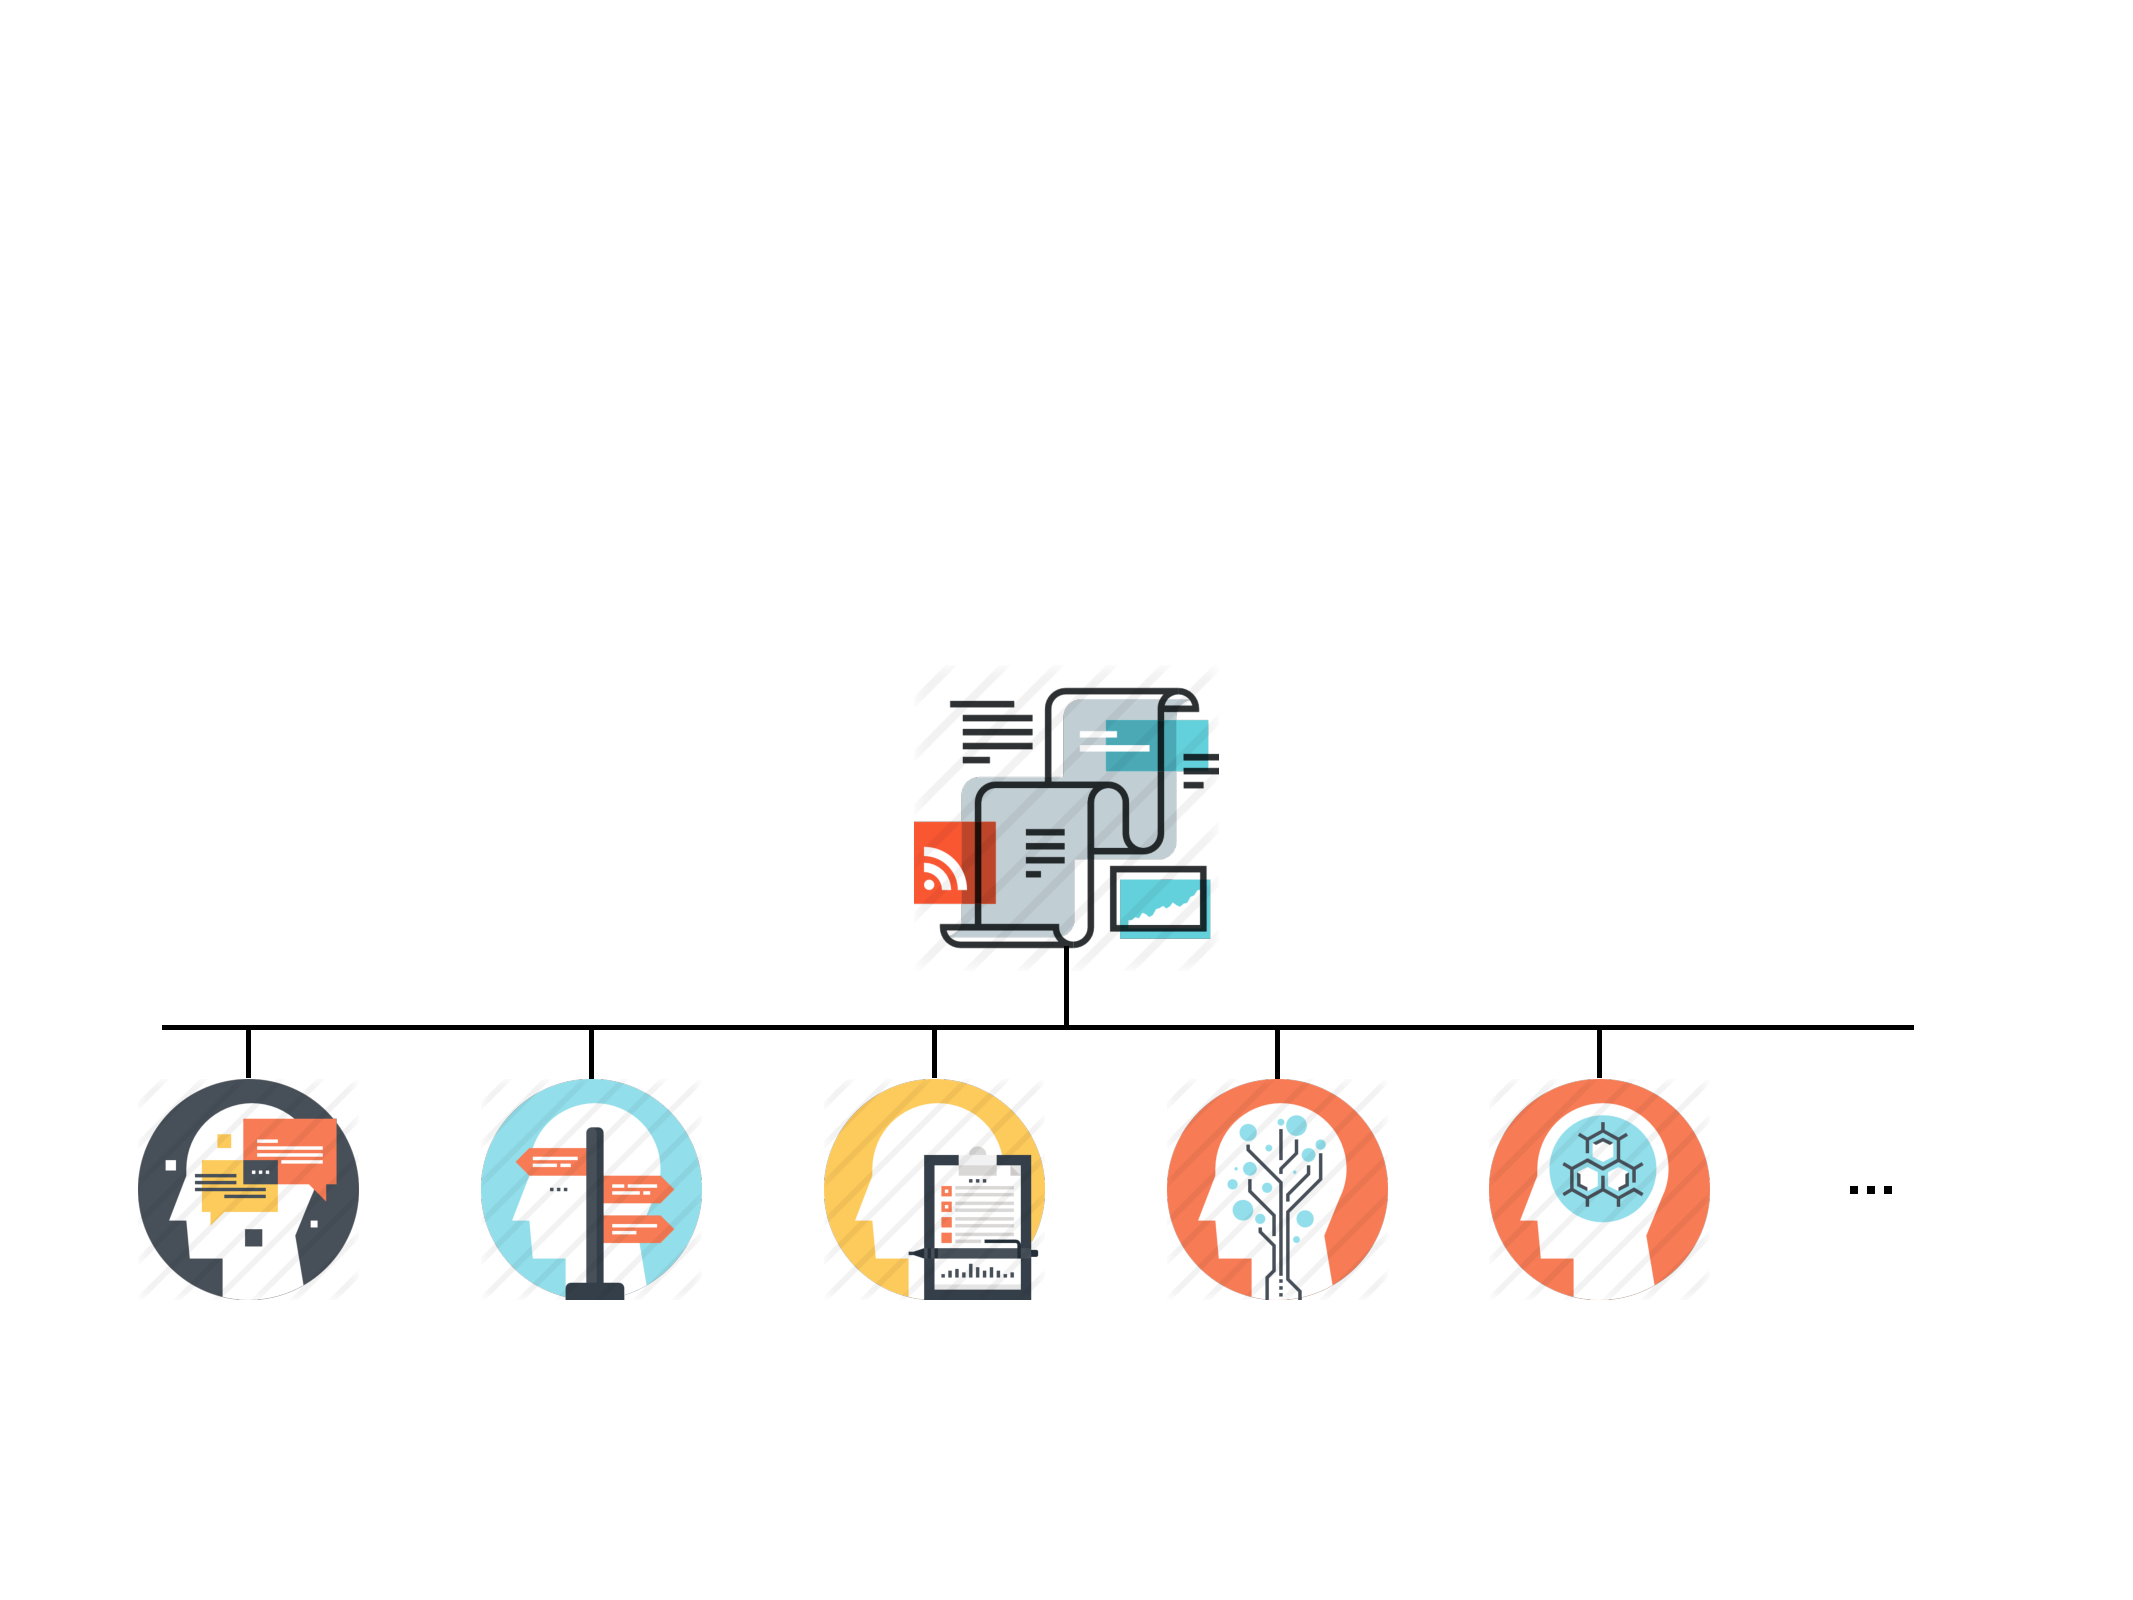
\includegraphics[width=1\textwidth]{figures/brain/rpg}
      \end{center}
    \end{block}}
  \only<2>{
    \begin{block}{\itbf{Reason 2}}
      \vskip4pt
      {\bhand} \emph{Ensuring their safety is \alert{desirable} and \alert{significant}.}
      \vskip2pt
      \begin{center}
        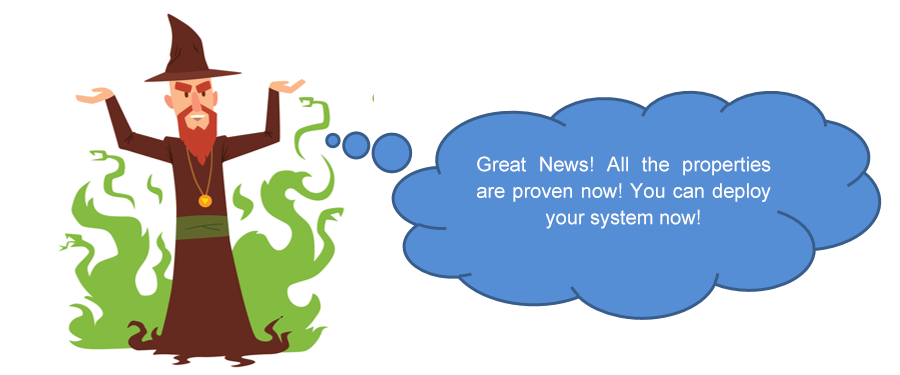
\includegraphics[width=0.7\textwidth]{figures/brain/magician}
      \end{center}
    \end{block}
  }

  \only<3>{
    \begin{block}{\itbf{However, ...}}
      \vskip4pt
      {\bhand} \emph{resource-parameterized program analysis is \alert{challenging}.} 
      \vskip6pt
      \begin{columns}
        \begin{column}{0.58\textwidth}
          \begin{center}
            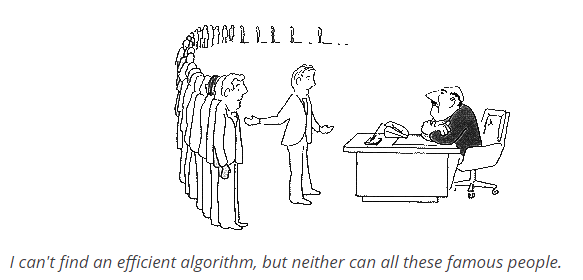
\includegraphics[width=\textwidth]{figures/brain/undecidable}
          \end{center}
        \end{column}
        \begin{column}{0.4\textwidth}
          \begin{center}
            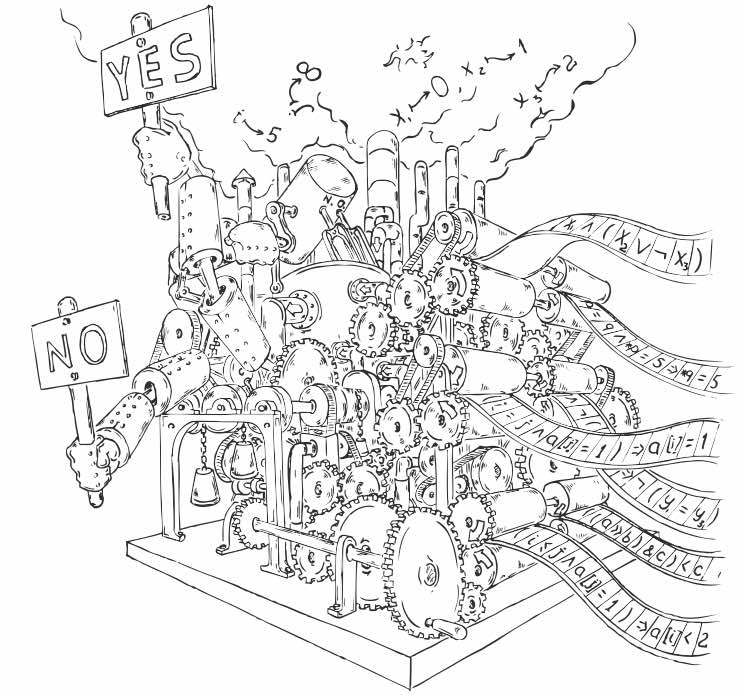
\includegraphics[width=0.75\textwidth]{figures/brain/challenge}
          \end{center}
        \end{column}
      \end{columns}
      \begin{columns}
        \begin{column}{0.58\textwidth}
          \begin{center}
            \emph{\scriptsize \alert{intractable}}
          \end{center}
        \end{column}
        \begin{column}{0.4\textwidth}
          \begin{center}
            \emph{\scriptsize or even \alert{undecidable}}
          \end{center}
        \end{column}
      \end{columns}   
    \end{block}}
\end{frame}

\begin{frame}
  \frametitle{A Sidestep}
  \only<1>{
    \begin{block}{\textit{\textit{Resource-bounded analysis}}}
      \vskip6pt
      \begin{center}
        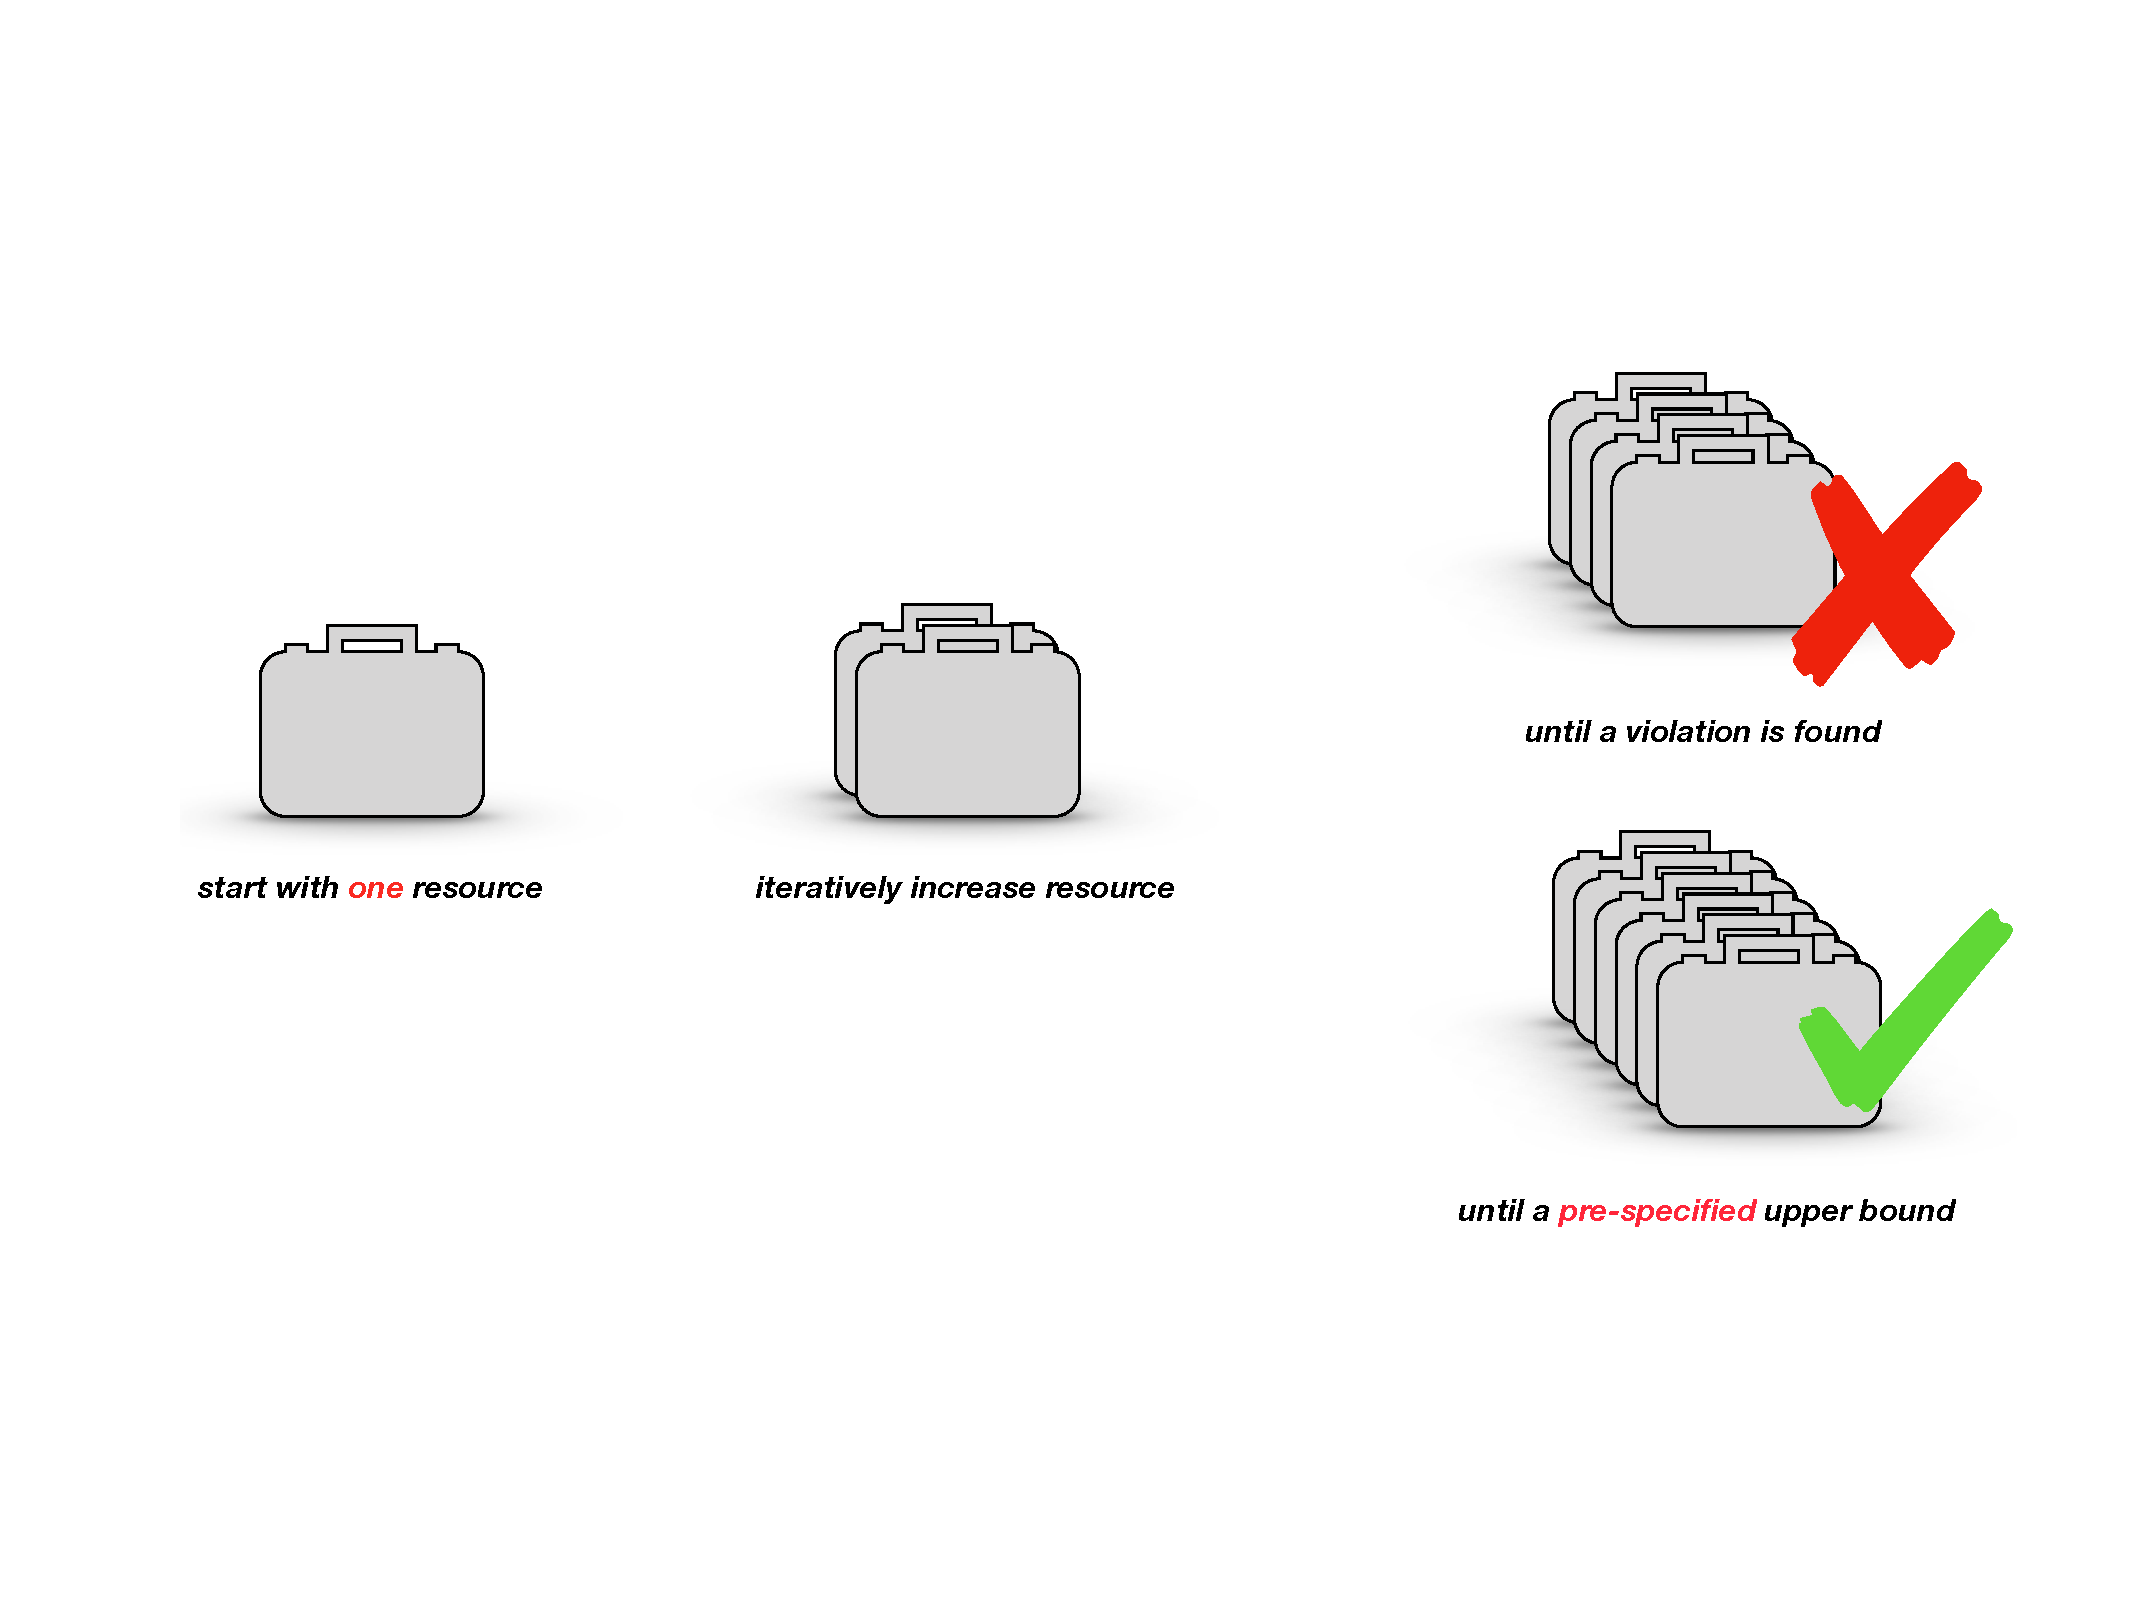
\includegraphics[width=0.9\textwidth]{figures/brain/rba}
      \end{center}
    \end{block}
  }
  \only<2>{
    \begin{block}{\textit{\textit{Tested empirically~[ASPLOS'08]}}}
      \vskip4pt
      {\bhand} \emph{Most bugs can be exposed with a \alert{small} number of resources.}
    \end{block}
    \begin{block}{\textit{\textit{We thus have}}}
      \begin{center}
        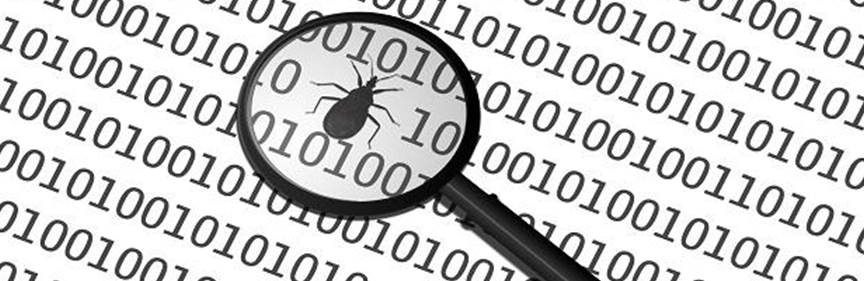
\includegraphics[width=0.75\textwidth]{figures/brain/bug-finding}\\
        \vskip6pt
        {\textbf{\textit{a \alert{bug-finding} technique}}}
     \end{center}
   \end{block}
  }
  \only<3>{
    \begin{block}{\emph{Still, uncertainty remains ...}}
      \vskip4pt
      {\bhand} \emph{beyond the pre-specified bound.}
      \vskip6pt
      \begin{center}
        
\includegraphics[width=0.55\textwidth]{figures/brain/bug}
     \end{center}
   \end{block}
 }
\end{frame}
 \begin{frame}
  \frametitle{Beyond the Sidestep}
  \only<1>{
    \begin{block}{\textit{\textit{Can we lift the bug-finding technique to resource-unbounded analysis?}}}
    \end{block}
    \begin{block}{}
      \vspace{-4pt}
      \begin{center}
        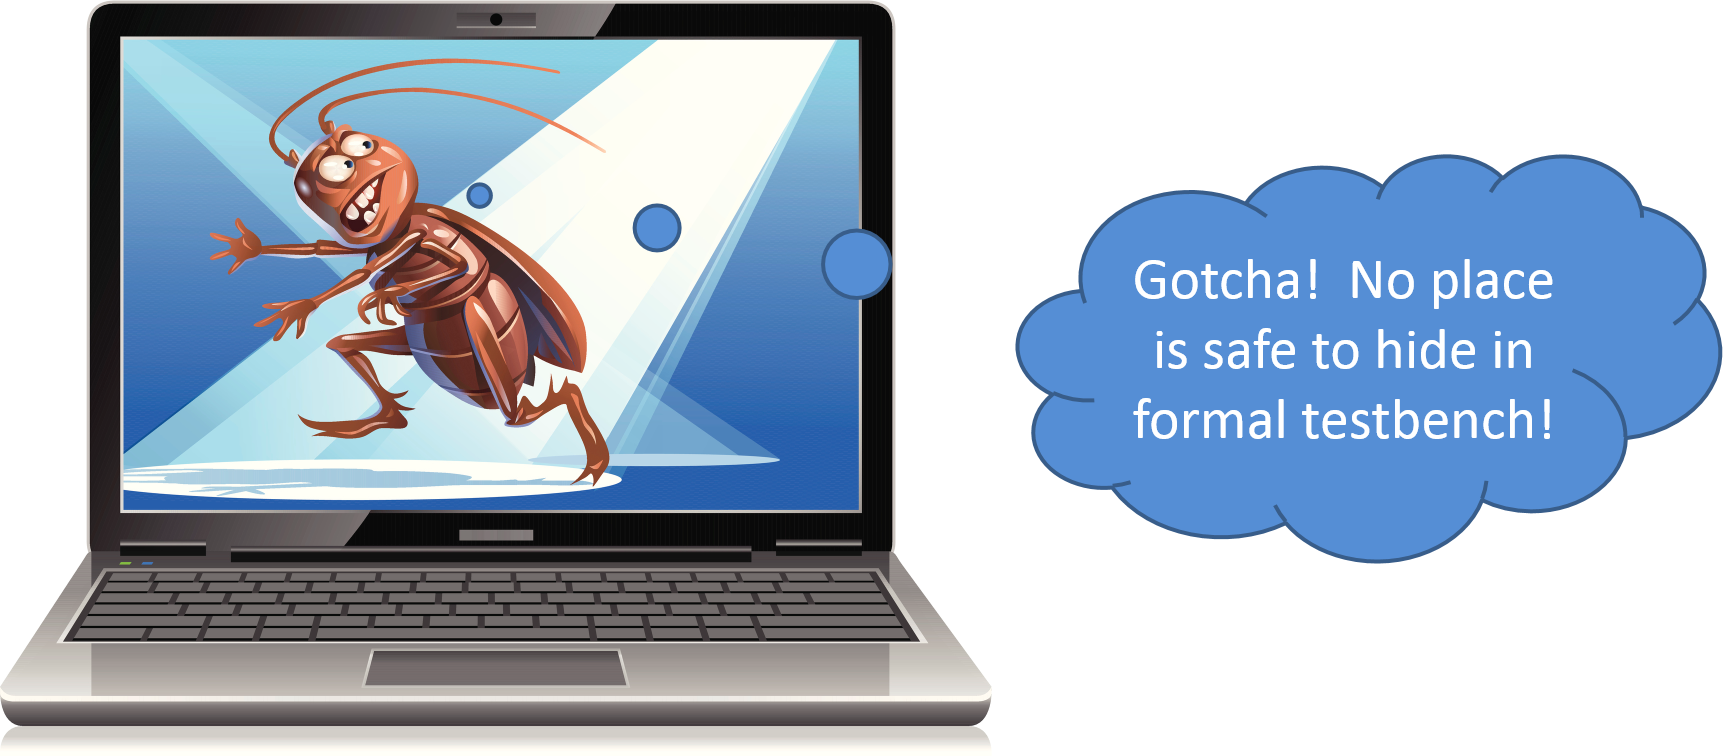
\includegraphics[width=0.55\textwidth]{figures/brain/nobug}
      \end{center}
    \end{block}
  }
\end{frame}

\begin{frame}
  \frametitle{Status of Research}
  \only<1>{
    \begin{block}{}%{\textit{Existing research}}
      \vspace{-10pt}
      \begin{center}
        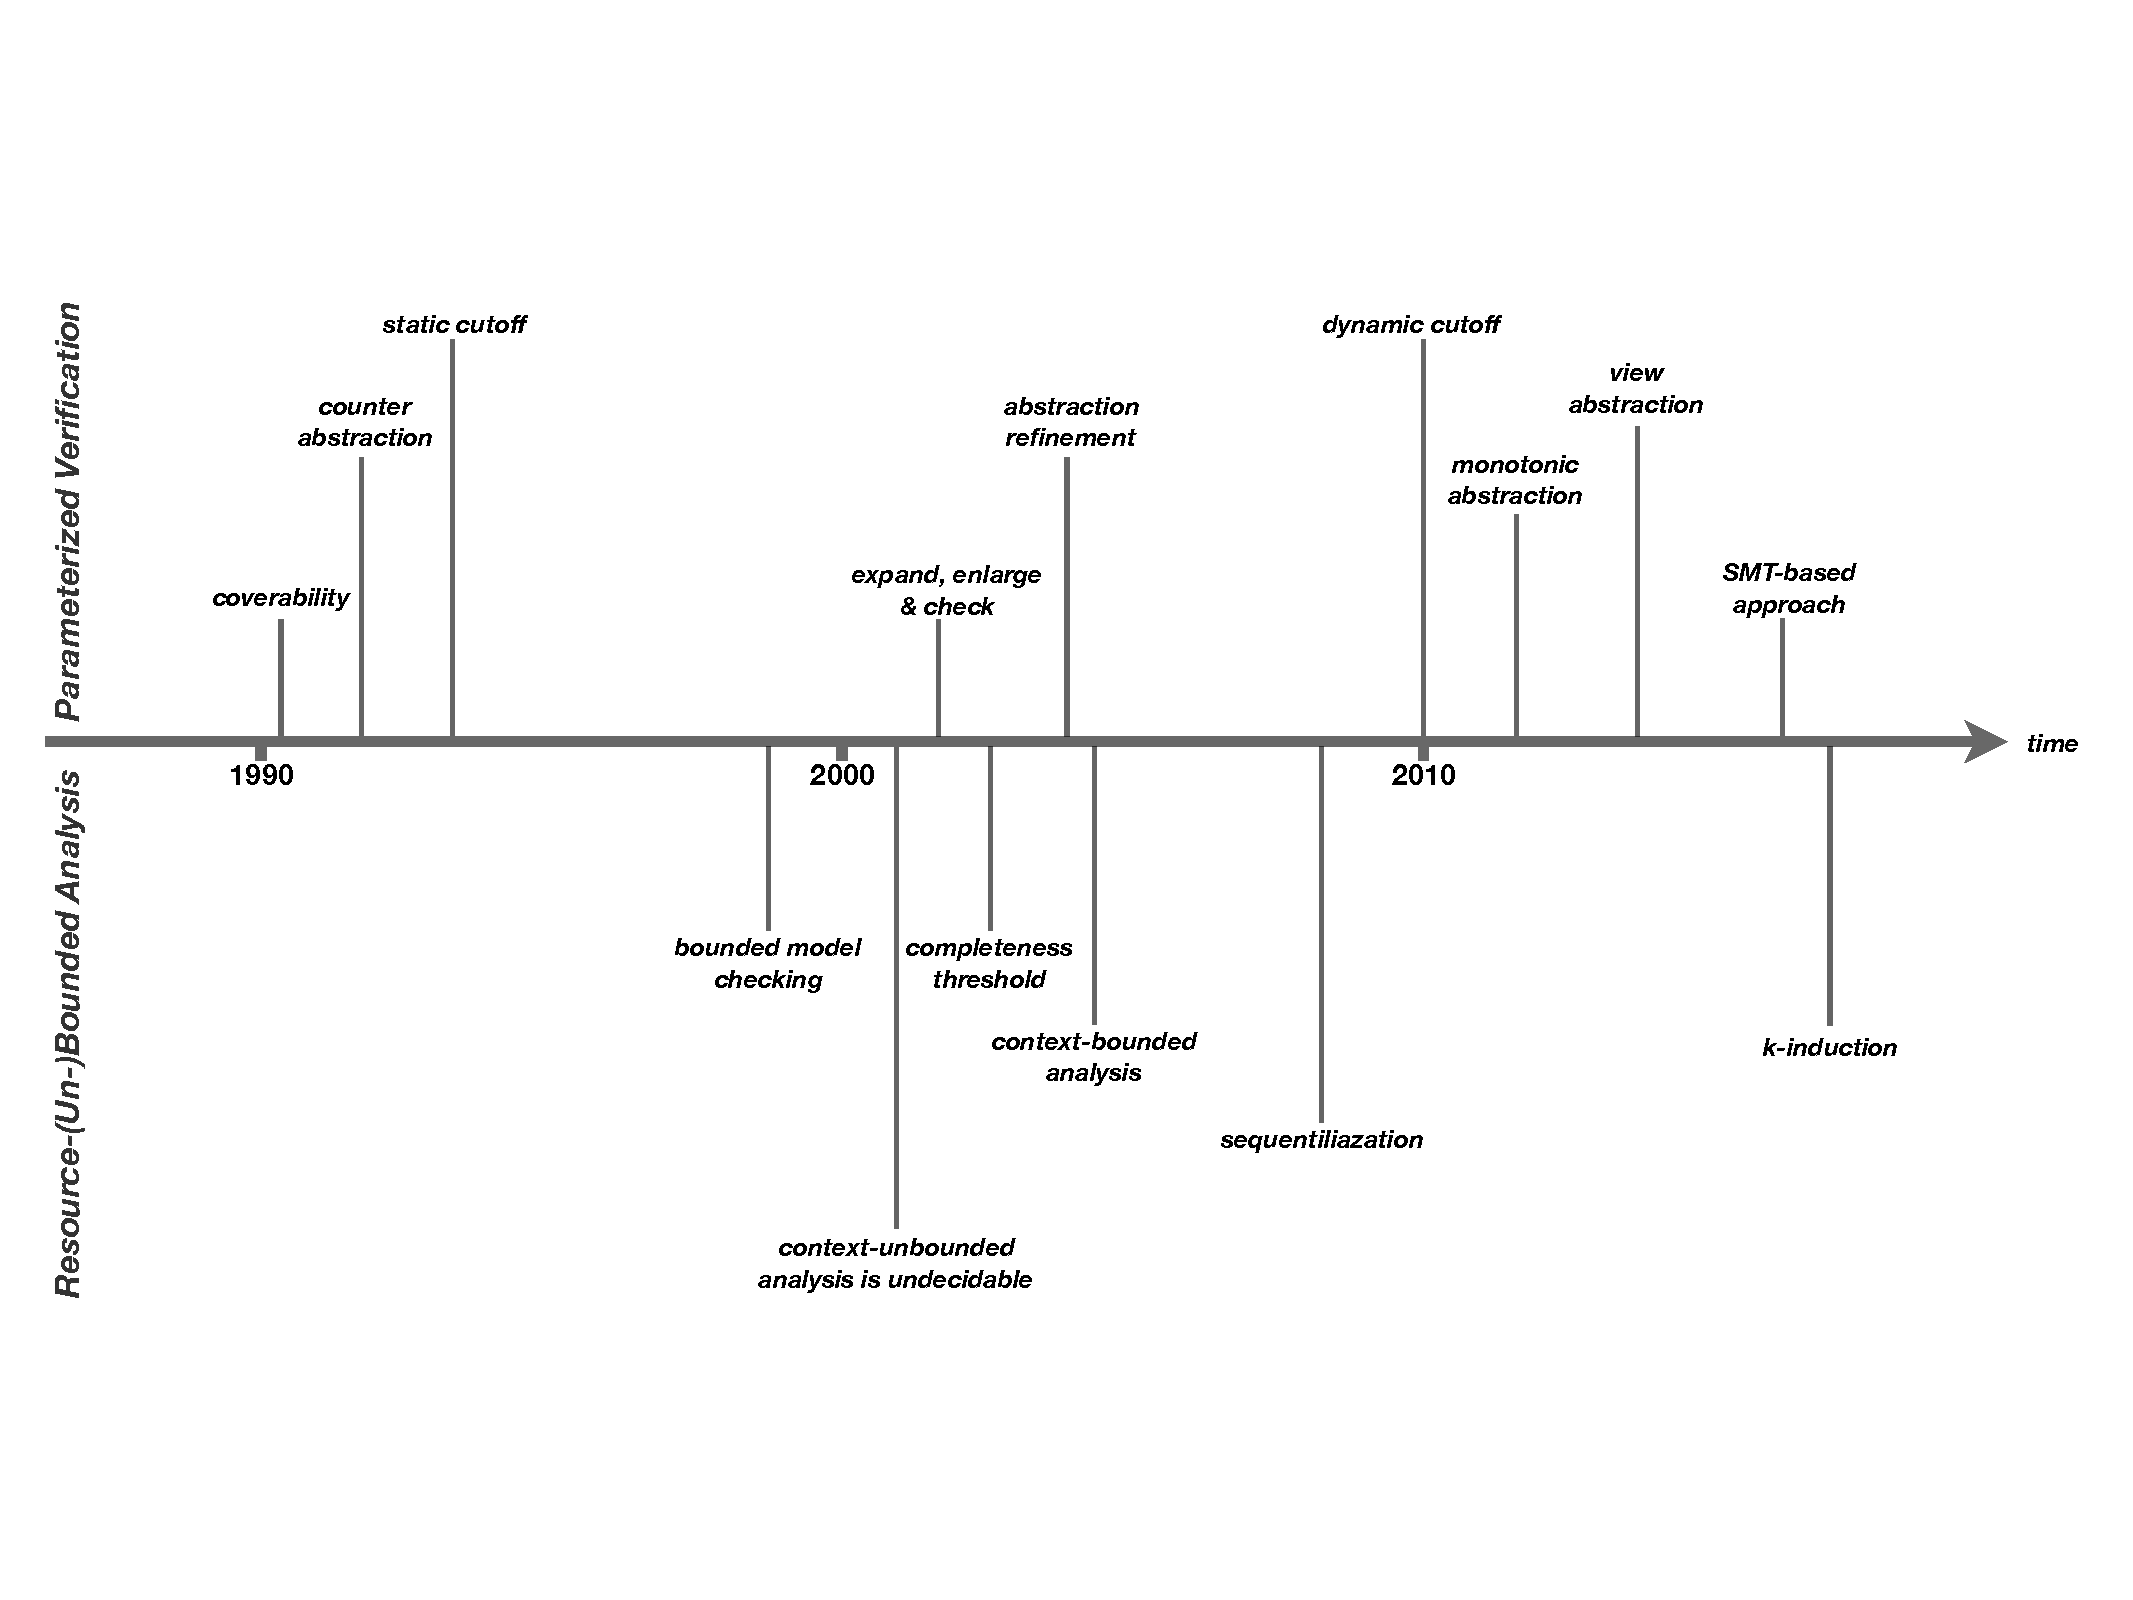
\includegraphics[width=1\textwidth]{figures/sor}
      \end{center}
    \end{block}}
  % \only<2>{
  %   \begin{block}{\textit{Existing research}}
  %     \begin{center}
  %       \includegraphics[width=0.9\textwidth]{figures/sor2}
  %     \end{center}
  %   \end{block}}
\end{frame}

\begin{frame}
  \frametitle{Research Goal}
  \begin{block}{\textit{To provide ...}}
    \vskip4pt
    {\bhand} \emph{a \alert{uniform} paradigm, which can}
      \begin{center}
        \emph{lift resource-bounded bug-finding technique to \alert{resource-unbounded analysis}.}
      \end{center}
  \end{block}
\end{frame}

%\section{A Motivating Example}
\begin{frame}
  \frametitle{Our Paradigm: Bird's Eye View}
  \only<1>{
    \begin{block}{\textit{Observation sequence (OS) ...}}
      \vskip4pt
     \emph{\small{Informally, a sequence of \alert{program behaviors} $\observation[k]$ observed within $k$ instances of resource.}}
    \end{block}
    % \begin{block}{\textit{As a (fairly natural) requirement,}}
   %    \[
   %      \observation[k] \subseteq \observation[k+1]
   %    \]
   %    \begin{center}
   %      {\bf Monotonicity}
   %   \end{center}
   % \end{block}
   \begin{block}{\textit{Examples}}
     \begin{enumerate}[\bhand]
     \item
        $\observation[k]$ := \{\emph{ reachable program \alert{states} within $k$ threads}\}
    \item
        $\observation[k]$ := \{\emph{ reachable program \alert{locations} within $k$ threads}\}
    \item ...
    \end{enumerate}
   \end{block}}
%    Put examples here: monotone and non-monotone ones. 
% \end{frame}

% \begin{frame}
%   \frametitle{Bird's Eye View}
 \only<2>{
   \begin{block}{Scheme}
     \centering
     \resizebox{0.7\textwidth}{!}{
       %%% Local Variables:
%%% mode: latex
%%% TeX-master: t
%%% End:

  \begin{tikzpicture}[%
    >=stealth,              % Nice arrows; your taste may be different
    start chain=going below,    % General flow is top-to-bottom
    node distance=6mm and 60mm, % Global setup of box spacing
    every join/.style={norm}]
    \tikzset{
      base/.style={draw, on chain, on grid, align=center, minimum height=4ex},
      proc/.style={base, rectangle, rounded corners},
      test/.style={base, diamond, aspect=2, rounded corners},
      term/.style={proc, draw=none},
      norm/.style={->, draw}
    }
    \node [term] (p0)
    {program $\pds$,
      property $\property$\\
      resource parameter $i:=0$
    };
    \node [proc, join] (Ok) {construct $\observation[i]$};
    \node [test, join] (violation) {$\observation[i]$ witnesses\\ a violation of $\property$?};
    \node [term, fill=red!60] (incorrect) {$\pds \not\models \property$};
    \node [proc, left=of Ok](kpp)  {$i := i + 1$};
    \node [test] (converge) {sequence {\scriptsize $\OS$}\\ \alert{converges} at $i$?};
    \node [term, fill=green!60] (correct) {$\pds \models \property$};

    \path (converge.north) to node [xshift=0.8em,yshift=0em] {\emph{no}} (kpp); 
    \draw [->] (converge.north) -- (kpp);
    \path (converge.south) to node [xshift=1em,yshift=0em] {\emph{yes}} (correct); 
    \draw [->] (converge.south) -- (correct);
    \path (violation.west) to node [xshift=0em,yshift=0.5em] {\emph{no}} (converge); 
    \draw [->] (violation.west) -- (converge);
    \path (violation.south) to node [xshift=1em,yshift=0em] {\emph{yes}} (incorrect); 
    \draw [->] (violation.south) -- (incorrect);
    \draw [->,shorten <=1pt,shorten >=1pt] (kpp.east) -- (Ok);
  \end{tikzpicture}
     }
   \end{block}}
\end{frame}

\section{A Paradigm: Observation Sequences}
\begin{frame}
  \frametitle{Observation Sequences}
  \begin{definition}
    \vskip4pt
    \label{definition: observation sequence}
    An \emphdef{observation sequence} is a sequence $\OS$ with the following
    properties:
    \begin{enumerate}[$\bullet$]
    \item%{\bf \emph{monotonicity~:}}
      \emph{for all $k$, $\observation_k \subseteq \observation_{k+1}$, that is \alert{monotonicity}.} 

    \item%{\bf \emph{computability:}}
      \emph{for all $k$, $\observation_k$ is \alert{computable}}. 

    \item%{\bf \emph{expressibility:}}
      \emph{for all $k$, $\observation[k] \models \property$ is \alert{decidable}, where $\property$ is a property of interest}.
    \end{enumerate}
  \end{definition}
\end{frame}

\begin{frame}
  \frametitle{Convergence Detection is Challenging}
  \begin{block}{}%{\textit{A possible approach}} \vskip4pt
    \begin{columns}
      \begin{column}{0.49\textwidth}
        \begin{center}
          % 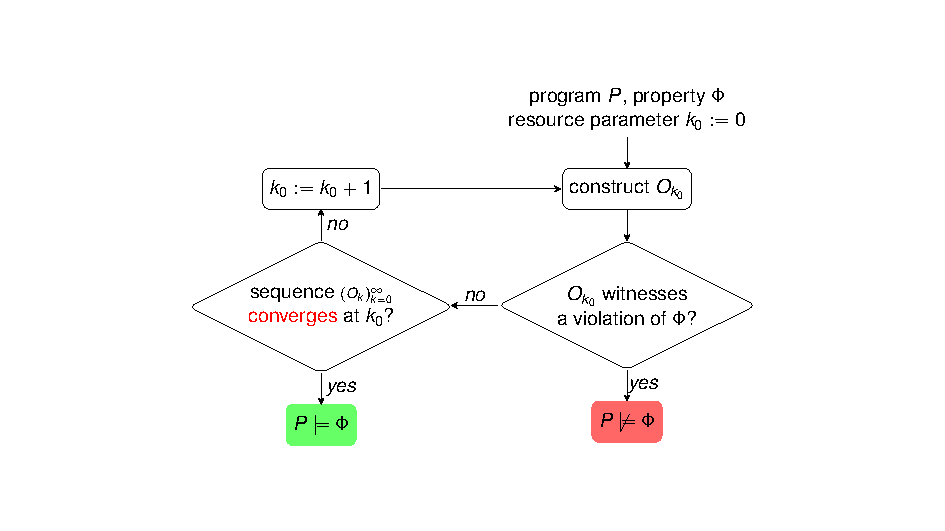
\includegraphics[width=1\textwidth]{figures/overview}
          \resizebox{1\textwidth}{!}{
            %%% Local Variables:
%%% mode: latex
%%% TeX-master: t
%%% End:

  \begin{tikzpicture}[%
    >=stealth,              % Nice arrows; your taste may be different
    start chain=going below,    % General flow is top-to-bottom
    node distance=6mm and 60mm, % Global setup of box spacing
    every join/.style={norm}]
    \tikzset{
      base/.style={draw, on chain, on grid, align=center, minimum height=4ex},
      proc/.style={base, rectangle, rounded corners},
      test/.style={base, diamond, aspect=2, rounded corners},
      term/.style={proc, draw=none},
      norm/.style={->, draw}
    }
    \node [term] (p0)
    {program $\pds$,
      property $\property$\\
      resource parameter $i:=0$
    };
    \node [proc, join] (Ok) {construct $\observation[i]$};
    \node [test, join] (violation) {$\observation[i]$ witnesses\\ a violation of $\property$?};
    \node [term, fill=red!60] (incorrect) {$\pds \not\models \property$};
    \node [proc, left=of Ok](kpp)  {$i := i + 1$};
    \node [test] (converge) {sequence {\scriptsize $\OS$}\\ \alert{converges} at $i$?};
    \node [term, fill=green!60] (correct) {$\pds \models \property$};

    \path (converge.north) to node [xshift=0.8em,yshift=0em] {\emph{no}} (kpp); 
    \draw [->] (converge.north) -- (kpp);
    \path (converge.south) to node [xshift=1em,yshift=0em] {\emph{yes}} (correct); 
    \draw [->] (converge.south) -- (correct);
    \path (violation.west) to node [xshift=0em,yshift=0.5em] {\emph{no}} (converge); 
    \draw [->] (violation.west) -- (converge);
    \path (violation.south) to node [xshift=1em,yshift=0em] {\emph{yes}} (incorrect); 
    \draw [->] (violation.south) -- (incorrect);
    \draw [->,shorten <=1pt,shorten >=1pt] (kpp.east) -- (Ok);
  \end{tikzpicture}
            }
        \end{center}
      \end{column}
      \begin{column}{0.49\textwidth}
        \begin{center}{\scriptsize  \textbf{\textit{Divergence}}}
          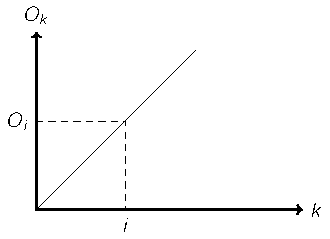
\includegraphics[width=1\textwidth]{figures/diverge}
        \end{center}
      \end{column}
    \end{columns}
  \end{block}
\end{frame}

\begin{frame}
  \frametitle{Abstraction}
  \begin{block}{}%{\textit{Well, not quite ...}}
    \begin{columns}
      \begin{column}{0.45\textwidth}
        \begin{center}{\scriptsize  \textbf{\textit{Divergence}}}
          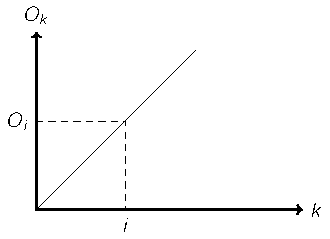
\includegraphics[width=1\textwidth]{figures/diverge}
        \end{center}
      \end{column}
      \begin{column}{0.12\textwidth}
        \begin{center}
          \alert{$\xrightarrow[]{\small{abstraction}}$}
        \end{center}
      \end{column}
      \begin{column}{0.45\textwidth}
        \begin{center}{\scriptsize \textbf{\textit{Convergence}}}
          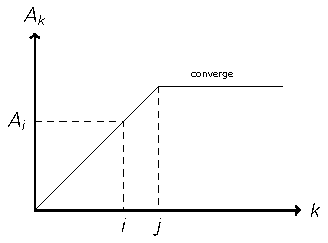
\includegraphics[width=1\textwidth]{figures/stutter-free}
        \end{center}
      \end{column}
    \end{columns}
  \end{block}
    \[
      A_k := abstraction(\observation[k])
      \]
\end{frame}

\begin{frame}
  \frametitle{Convergence Property}
  % \begin{block}{}
  %   \emph{An OS $\OS$ over a \alert{finite} domain always converges.}
  % \end{block}
  \begin{block}{}
    \begin{center}
      % {\rhand} \emph{$\OS$ converges $\not\Rightarrow$ Its domain is finite!}
      \emph{An OS $\OS$ over a \alert{finite} domain always converges.}
    \end{center}
  \end{block}
\end{frame}

\begin{frame}
  \frametitle{Stuttering}
  \begin{block}{}%{\textit{Well, not quite ...}}
    \begin{columns}
      \begin{column}{0.45\textwidth}
        \begin{center}{\scriptsize  \textbf{\textit{Divergence}}}
          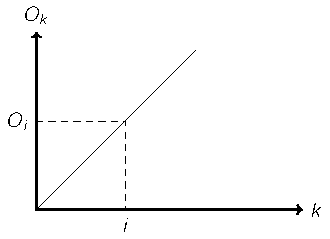
\includegraphics[width=1\textwidth]{figures/diverge}
        \end{center}
      \end{column}
      \begin{column}{0.12\textwidth}
        \begin{center}
          \alert{$\xrightarrow[]{\small{abstraction}}$}
        \end{center}
      \end{column}
      \begin{column}{0.45\textwidth}
        \begin{center}{\scriptsize \textbf{\textit{Stuttering}}}
          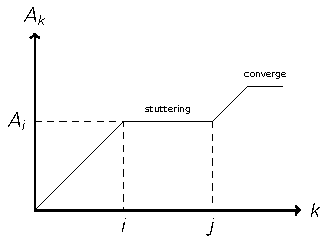
\includegraphics[width=1\textwidth]{figures/stuttering}
        \end{center}
      \end{column}
    \end{columns}
    \[
      A_k := abstraction(\observation[k])
      \]
  \end{block}
\end{frame}

% \begin{frame}
%   \frametitle{Challenges in Convergence Detection}
%   \only<1>{
%     \begin{block}{\textit{But why ...}}
%       \begin{columns}
%         \begin{column}{0.45\textwidth}
%           \begin{center}{\scriptsize  \textbf{\textit{divergence?}}}
%             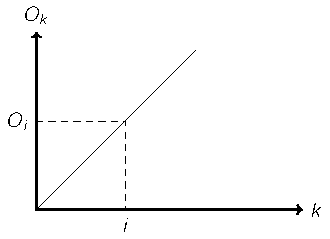
\includegraphics[width=1\textwidth]{figures/diverge}
%           \end{center}
%         \end{column}
%         \begin{column}{0.45\textwidth}
%           \begin{center}{\scriptsize \textbf{\textit{stuttering?}}}
%             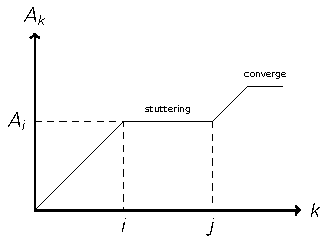
\includegraphics[width=1\textwidth]{figures/stuttering}
%           \end{center}
%         \end{column}
%       \end{columns}
%     \end{block}}
%   \only<2>{
%     \begin{block}{\textit{Because ...}}
%       \begin{columns}
%         \begin{column}{0.45\textwidth}
%           \begin{center}{\scriptsize  \textbf{\textit{divergence}}}
%             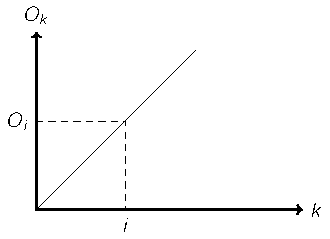
\includegraphics[width=1\textwidth]{figures/diverge}
%           \end{center}
%         \end{column}
%         \begin{column}{0.45\textwidth}
%           \begin{center}{\scriptsize \textbf{\textit{stuttering}}}
%             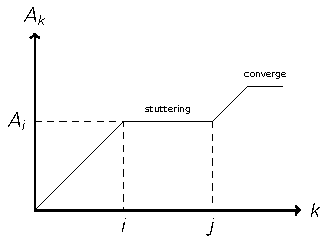
\includegraphics[width=1\textwidth]{figures/stuttering}
%           \end{center}
%         \end{column}
%       \end{columns}
%     \begin{columns}
%       \begin{column}{0.45\textwidth}
%         \begin{center}
%           {\scriptsize \textbf{\textit{\alert{infinite domain ...}}}}
%         \end{center}
%       \end{column}
%       \begin{column}{0.45\textwidth}
%         \begin{center}
%           {\scriptsize \textbf{\textit{\alert{abstraction, information lost ...}}}}
%         \end{center}
%       \end{column}
%     \end{columns}
%     \end{block}}
% \end{frame}

\begin{frame}
  \frametitle{Convergence}
  \only<1>{
    \begin{block}{}%{\textit{Two Possibilities}}
      \begin{columns}
        \begin{column}{0.45\textwidth}
          \begin{center}{\scriptsize  \textbf{\textit{stuttering}}}
            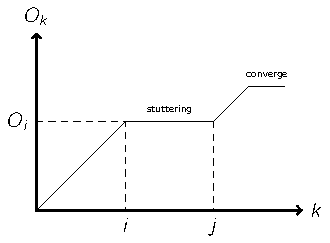
\includegraphics[width=1\textwidth]{figures/stt}
          \end{center}
        \end{column}
        \begin{column}{0.45\textwidth}
          \begin{center}{\scriptsize \textbf{\textit{stutter-free}}}
            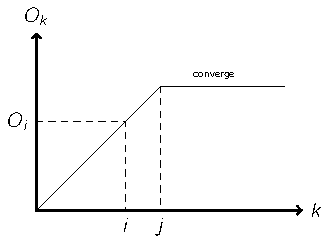
\includegraphics[width=1\textwidth]{figures/sfr}
          \end{center}
        \end{column}
      \end{columns}
    \end{block}}
\end{frame}

\begin{frame}
  \frametitle{A Refined Scheme}
  \centering
  \resizebox{0.8\textwidth}{!}{
  \begin{tikzpicture}[%
    >=stealth,              % Nice arrows; your taste may be different
    start chain=going below,    % General flow is top-to-bottom
    node distance=6mm and 60mm, % Global setup of box spacing
    every join/.style={norm}]
    \tikzset{
      base/.style={draw, on chain, on grid, align=center, minimum height=4ex},
      proc/.style={base, rectangle, rounded corners},
      test/.style={base, diamond, aspect=2, rounded corners},
      term/.style={proc, draw=none},
      norm/.style={->, draw}
    }
    \node [term] (p0)
    {program $\pds$,
     property $\property$\\
     resource parameter $i:=0$
    };
    \node [proc, join] (Ok) {construct $\observation[i]$};
    \node [test, join] (violation) {$\observation[i]$ witnesses\\ a violation of $\property$?};
    \node [term, fill=red!60] (incorrect) {$\pds \not\models \property$};
    \node [proc, left=of Ok](kpp)  {$i := i + 1$};
    \node [test, left=of violation, fill=blue!20] (converge) {$\observation[i-1] = \observation[i]$? };
    \node [test, left=of converge, fill=blue!20] (stutter) {sequence {\scriptsize $\OS$}\\ \alert{stutters} at $i$?};
    \node [term, fill=green!60] (correct) {$\pds \models \property$};

    \path (converge.north) to node [xshift=0.8em,yshift=0em] {\emph{no}} (kpp); 
    \draw [->] (converge.north) -- (kpp);
    \path (converge.west) to node [xshift=2.5em,yshift=3em] {\emph{yes}} (correct); 
    \draw [->] (converge.west) -- (stutter);
    \path (violation.west) to node [xshift=0em,yshift=0.5em] {\emph{no}} (converge); 
    \draw [->] (violation.west) -- (converge);
    \path (violation.south) to node [xshift=1em,yshift=0em] {\emph{yes}} (incorrect); 
    \draw [->] (violation.south) -- (incorrect);
    \path (stutter.south) to node [xshift=-13.8em,yshift=0.5em] {\emph{no}} (incorrect); 
    \draw [->] (stutter.south) -- (correct);
    \path (stutter.north) to node [xshift=-8.8em,yshift=7.7em] {\emph{yes}} (incorrect);
    \draw [-] (stutter.north) -- (-12,-1.5);
    \draw [->] (-12,-1.5) -- (kpp.west);
    \draw [->,shorten <=1pt,shorten >=1pt] (kpp.east) -- (Ok);
  \end{tikzpicture}
}
% \vskip10pt
% {\bhand} \emph{\scriptsize the case of \alert{stutter-free} is subsumed}
\end{frame}

\section{Application: Context-UnBounded Analysis}
\begin{frame}
  \frametitle{Context-UnBounded Analysis (CUBA)}
  \begin{block}{\emph{Target is ...}}
    \vskip2pt
    \emph{shared-memory multi-threaded \alert{recursive} programs.}
    \centering
  \end{block}
  \begin{block}{\emph{Resource is ...}}
    \vskip2pt
    \emph{the number of \alert{contexts} in the executions.}
    \centering
  \end{block}
  \begin{block}{\emph{Observation is ...}}
    \vskip2pt
    \emph{the set of \alert{reachable} program states w.r.t. $k$ contexts.}
    \centering
  \end{block}
  \begin{block}{\emph{Analysis is ...}}
    \vskip2pt
    \emph{to check the reachability of \alert{bad} states.}
    \centering
  \end{block}
\end{frame}

% \begin{frame}
%   \frametitle{Operational Model}
%   \only<1>{
%     \begin{block}{\emph{Pushdown System (PDS)}}
%       \vskip4pt
%       \emph{A PDS $\pds$ is a tuple $(\pdsshareds,\alphabet, \pdstranss, \pdsinitstate)$, where 
%         \begin{itemize}
%         \item $\pdsshareds$ is a set of states;
%         \item $\alphabet$ a finite stack alphabet;
%         \item $\pdstranss \subseteq (\pdsshareds \times \alphabetwithempty) \times (\pdsshareds \times \alphabetmaxtwo)$,
%           $\alphabetwithempty = \alphabet \union
%           \{\emptyword\}$ and $\alphabetmaxtwo = \{\word \in \Sigma^* \st |\word| \atm 2\}$
%         \item $\pdsinitstate \in \pdsshareds$ is the initial shared state. 
%         \end{itemize}
%       }
%     \end{block}
%   }
%   \only<2>{
%     \begin{block}{\emph{States}}
%       \vskip4pt
%       \emph{A state of $\pds$ is an element of $\pdsshareds \times \alphabet$.}
%     \end{block}
%     \begin{block}{}%{\emph{Vividly}}
%         \begin{center}
%           \includegraphics[width=0.3\textwidth]{figures/brain/pds-state}
%         \end{center}
%     \end{block}
%   }
% \end{frame}

 \begin{frame}
  \frametitle{Operational Model}
  \only<1>{
    \begin{block}{\emph{Concurrent Pushdown System (CPDS)}}
      \vskip2pt
      \emph{A CPDS $\pds^n$
        is a collection of $n$ PDS $\pds_i = (\pdsshareds,\alphabet_i,\pdstranss_i,\pdsinitstate)$, $1 \atm i \atm n$, where 
        \begin{enumerate}[$\bullet$]
        \item $\pdsshareds$ is a finite set of \alert{shared} states;
        \item $\alphabet_i$ is a finite set of \alert{local} states;
        \item $\pdstranss_i \subseteq (\pdsshareds \times \alphabet_i^{\atm 1}) \times (\pdsshareds \times \alphabet_i^{\atm 2})$,
          $\alphabet_i^{\atm 1} = \alphabet_i \union
          \{\emptyword\}$ and $\alphabet_i^{\atm 2} = \{\word \in \alphabet_i^* \st |\word| \atm 2\}$;
        \item $\pdsinitstate \in \pdsshareds$ is the initial shared state. 
        \end{enumerate}
        % The set $\pdsshareds$ of shared states is the same for all $\pds_i$.
      }
    \end{block}
  }
  \only<2>{
    \begin{block}{\emph{Semantics}}
        \begin{center}
          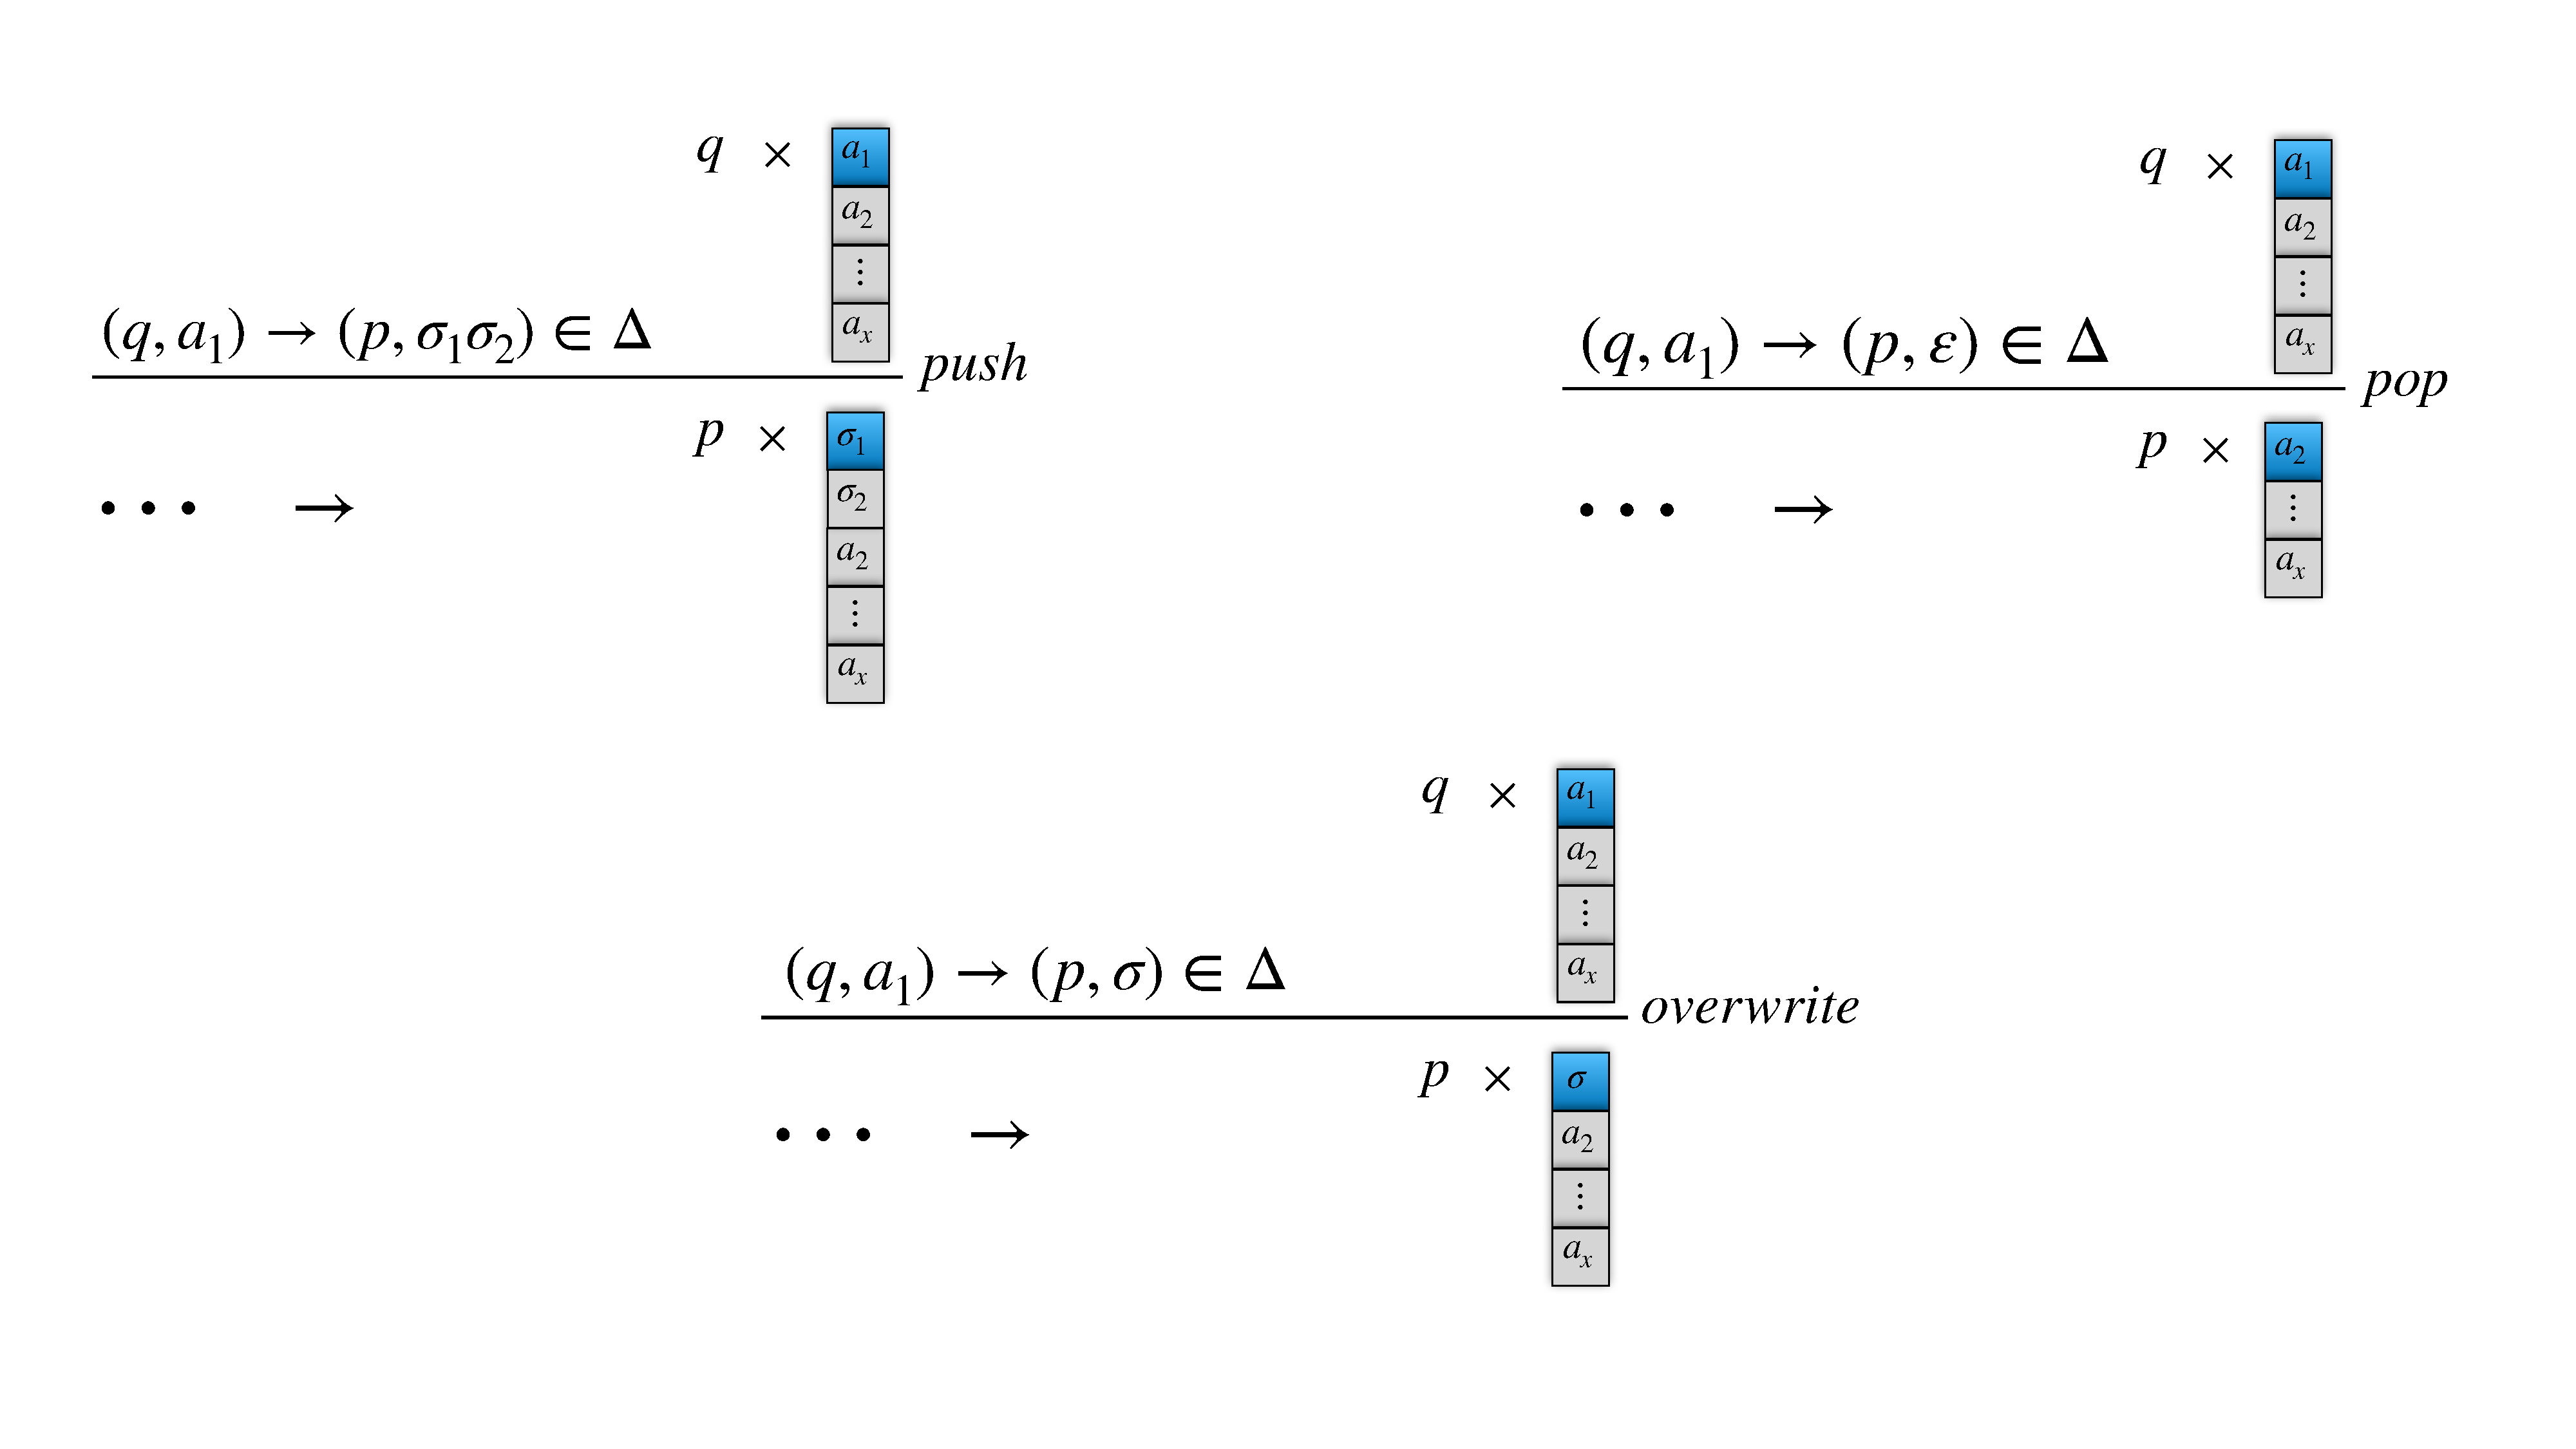
\includegraphics[width=.95\textwidth]{figures/brain/semantics}
        \end{center}
    \end{block}
  }
  \only<3>{
    \begin{block}{\emph{States}}
      \vskip4pt
      \emph{A \alert{global state} of a CPDS is an element of $\pdsshareds \times \alphabet_1^* \times \ldots \times \alphabet_n^*$, written in angle brackets: $\config q {\range[]{\word_1}{\word_n}}$.}
    \end{block}
    \begin{block}{\emph{For instance}}
        \begin{center}
          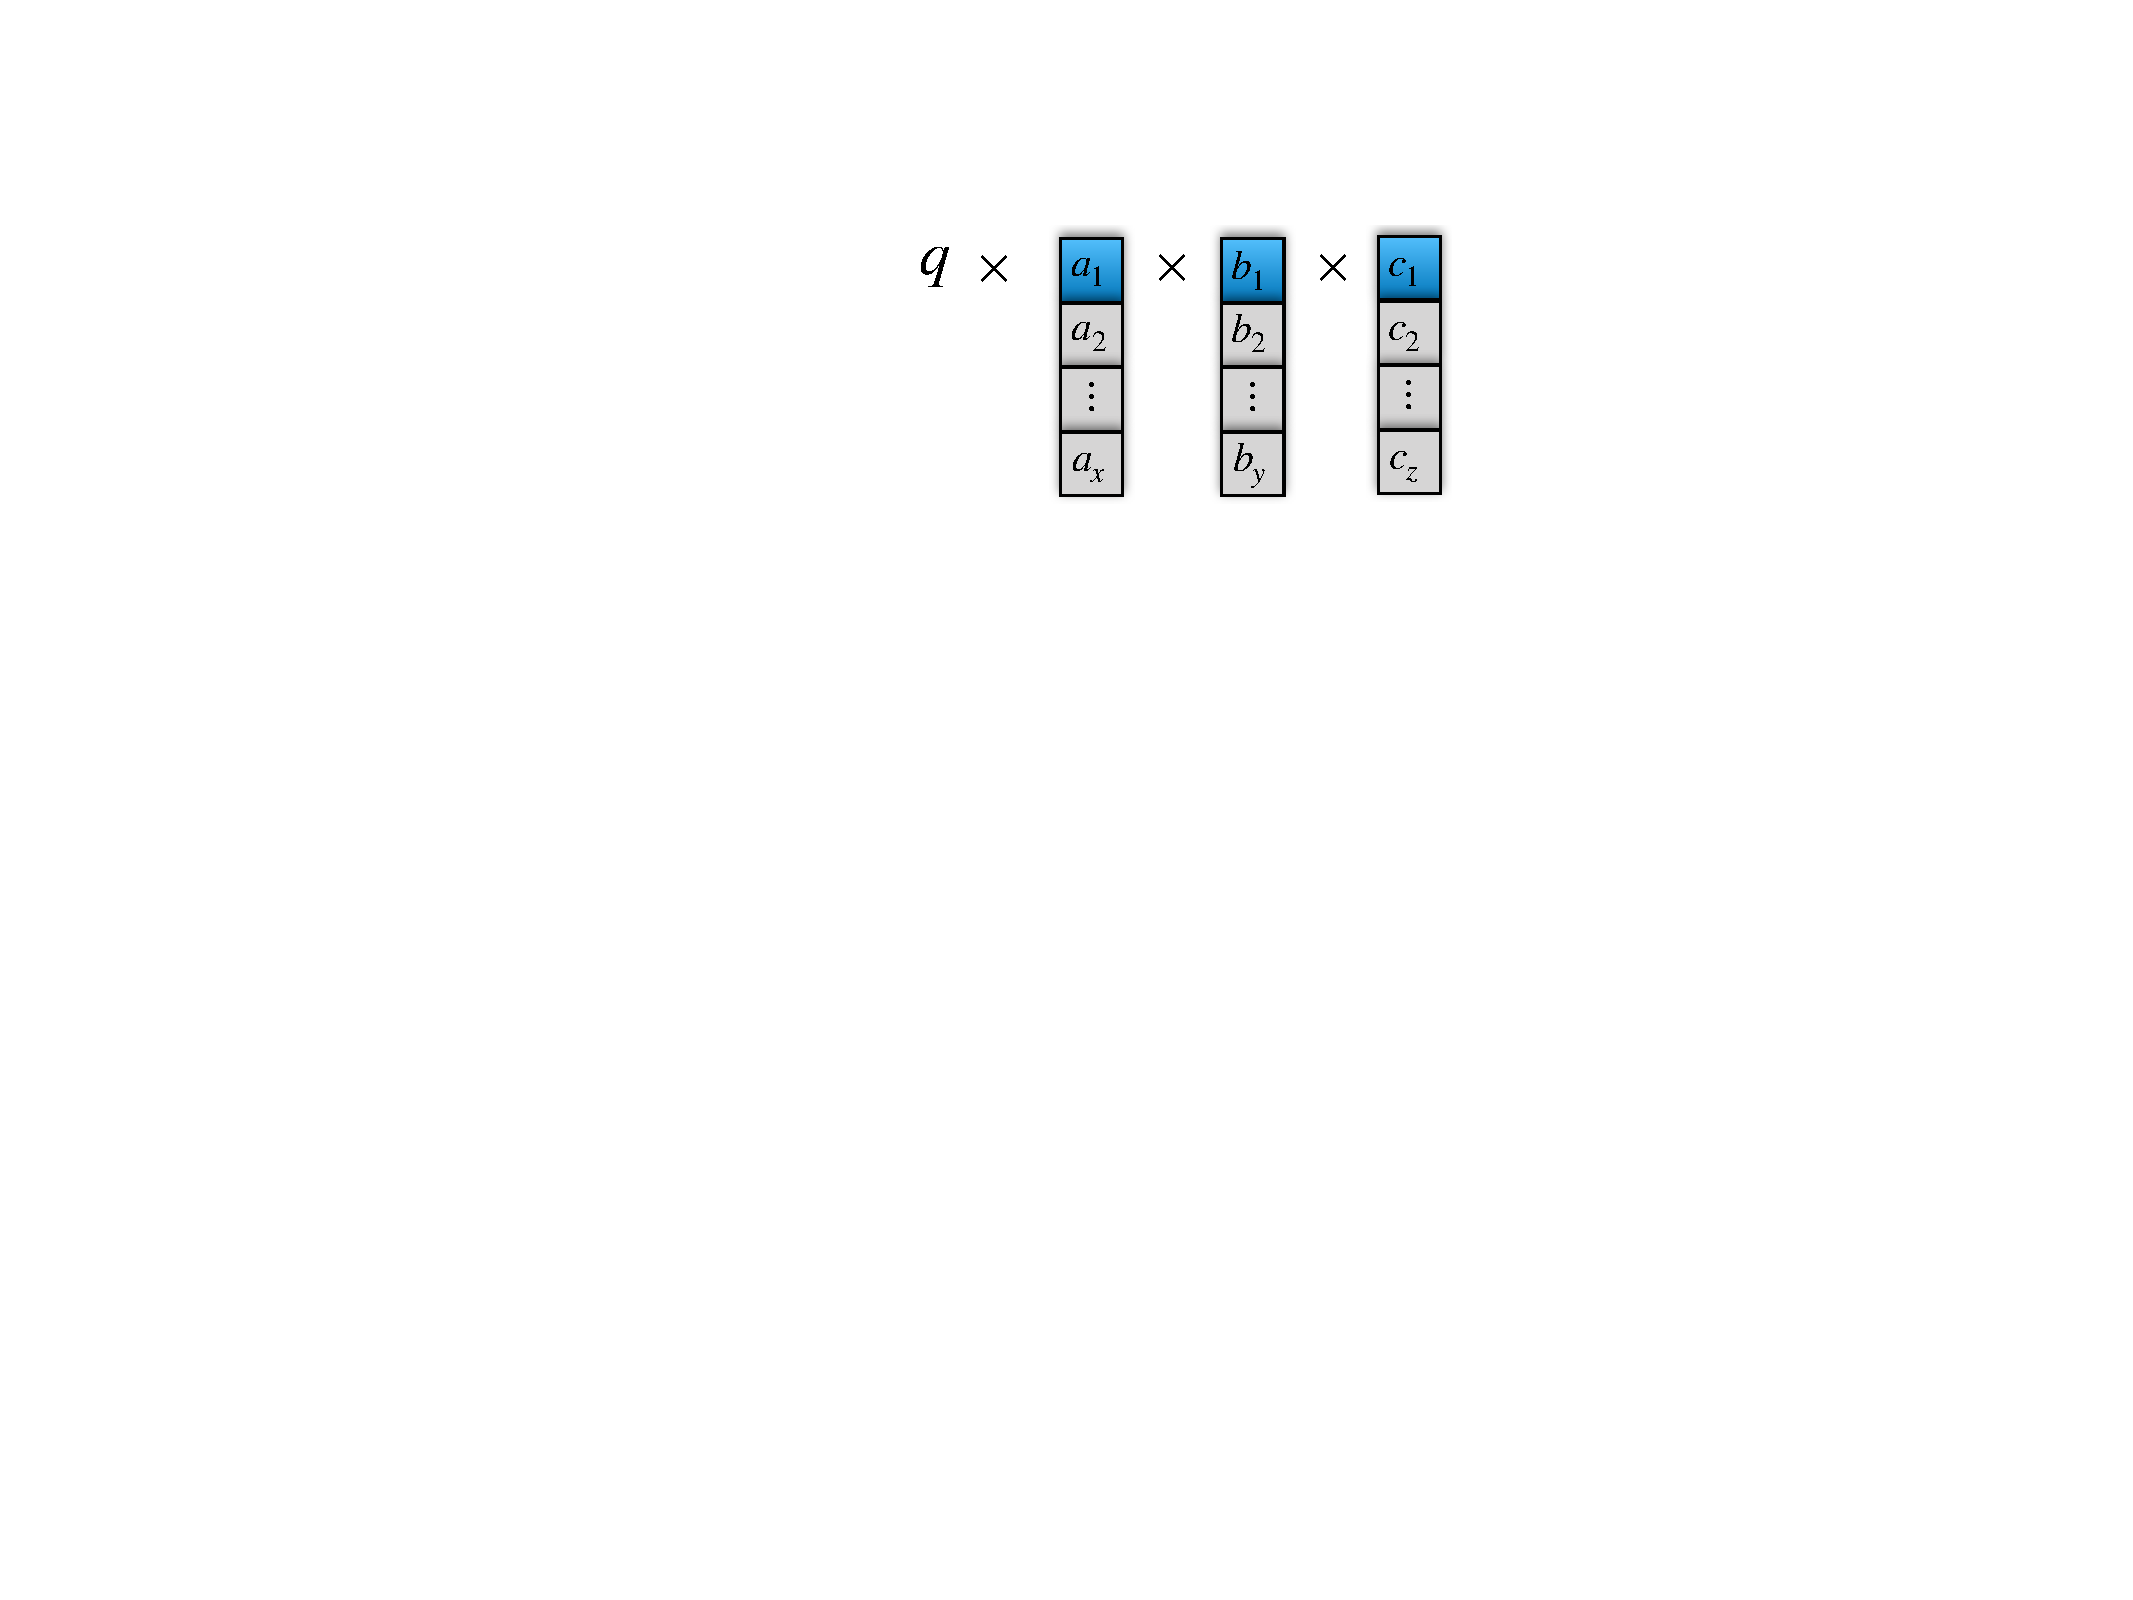
\includegraphics[width=0.4\textwidth]{figures/brain/cpds-state}
        \end{center}
    \end{block}
  }
  \only<4>{
    \begin{block}{\emph{Executions}}
    \[
    \begin{array}{llll}
      Thread\ A:\ \underbrace{\NO \rightarrow ... \rightarrow \NO \rightarrow}_{context} & &   \underbrace{\NO \rightarrow ... \rightarrow \NO \rightarrow}_{context} &\\
      Thread\ B:\ &  \underbrace{\NO \rightarrow ... \rightarrow \NO \rightarrow}_{context} & & \\
      Thread\ C:\ & & & \underbrace{\NO \rightarrow ... \rightarrow \NO \rightarrow}_{context} 
    \end{array}
    \]
    \end{block}
    \begin{block}{}%{\emph{Resource is }}
        \begin{center}
          \emph{resource := \alert{contexts}}
        \end{center}
    \end{block}
  }
\end{frame}

\begin{frame}
  \frametitle{Problem Statement}
  \only<1>{
    \begin{block}{\emph{A state is reachable if ...}}
      \[
        \begin{array}{ll}
          \underbrace{\NO}_{\textcolor{green!50!black!80}{initial}} \longrightarrow  \NO \longrightarrow \NO \longrightarrow \NO \longrightarrow ... \longrightarrow \NO \longrightarrow \underbrace{\YES}_{target} & \\
        \end{array}
      \]
    \end{block}
    \begin{block}{\emph{Safety as reachability}}
        \begin{center}
          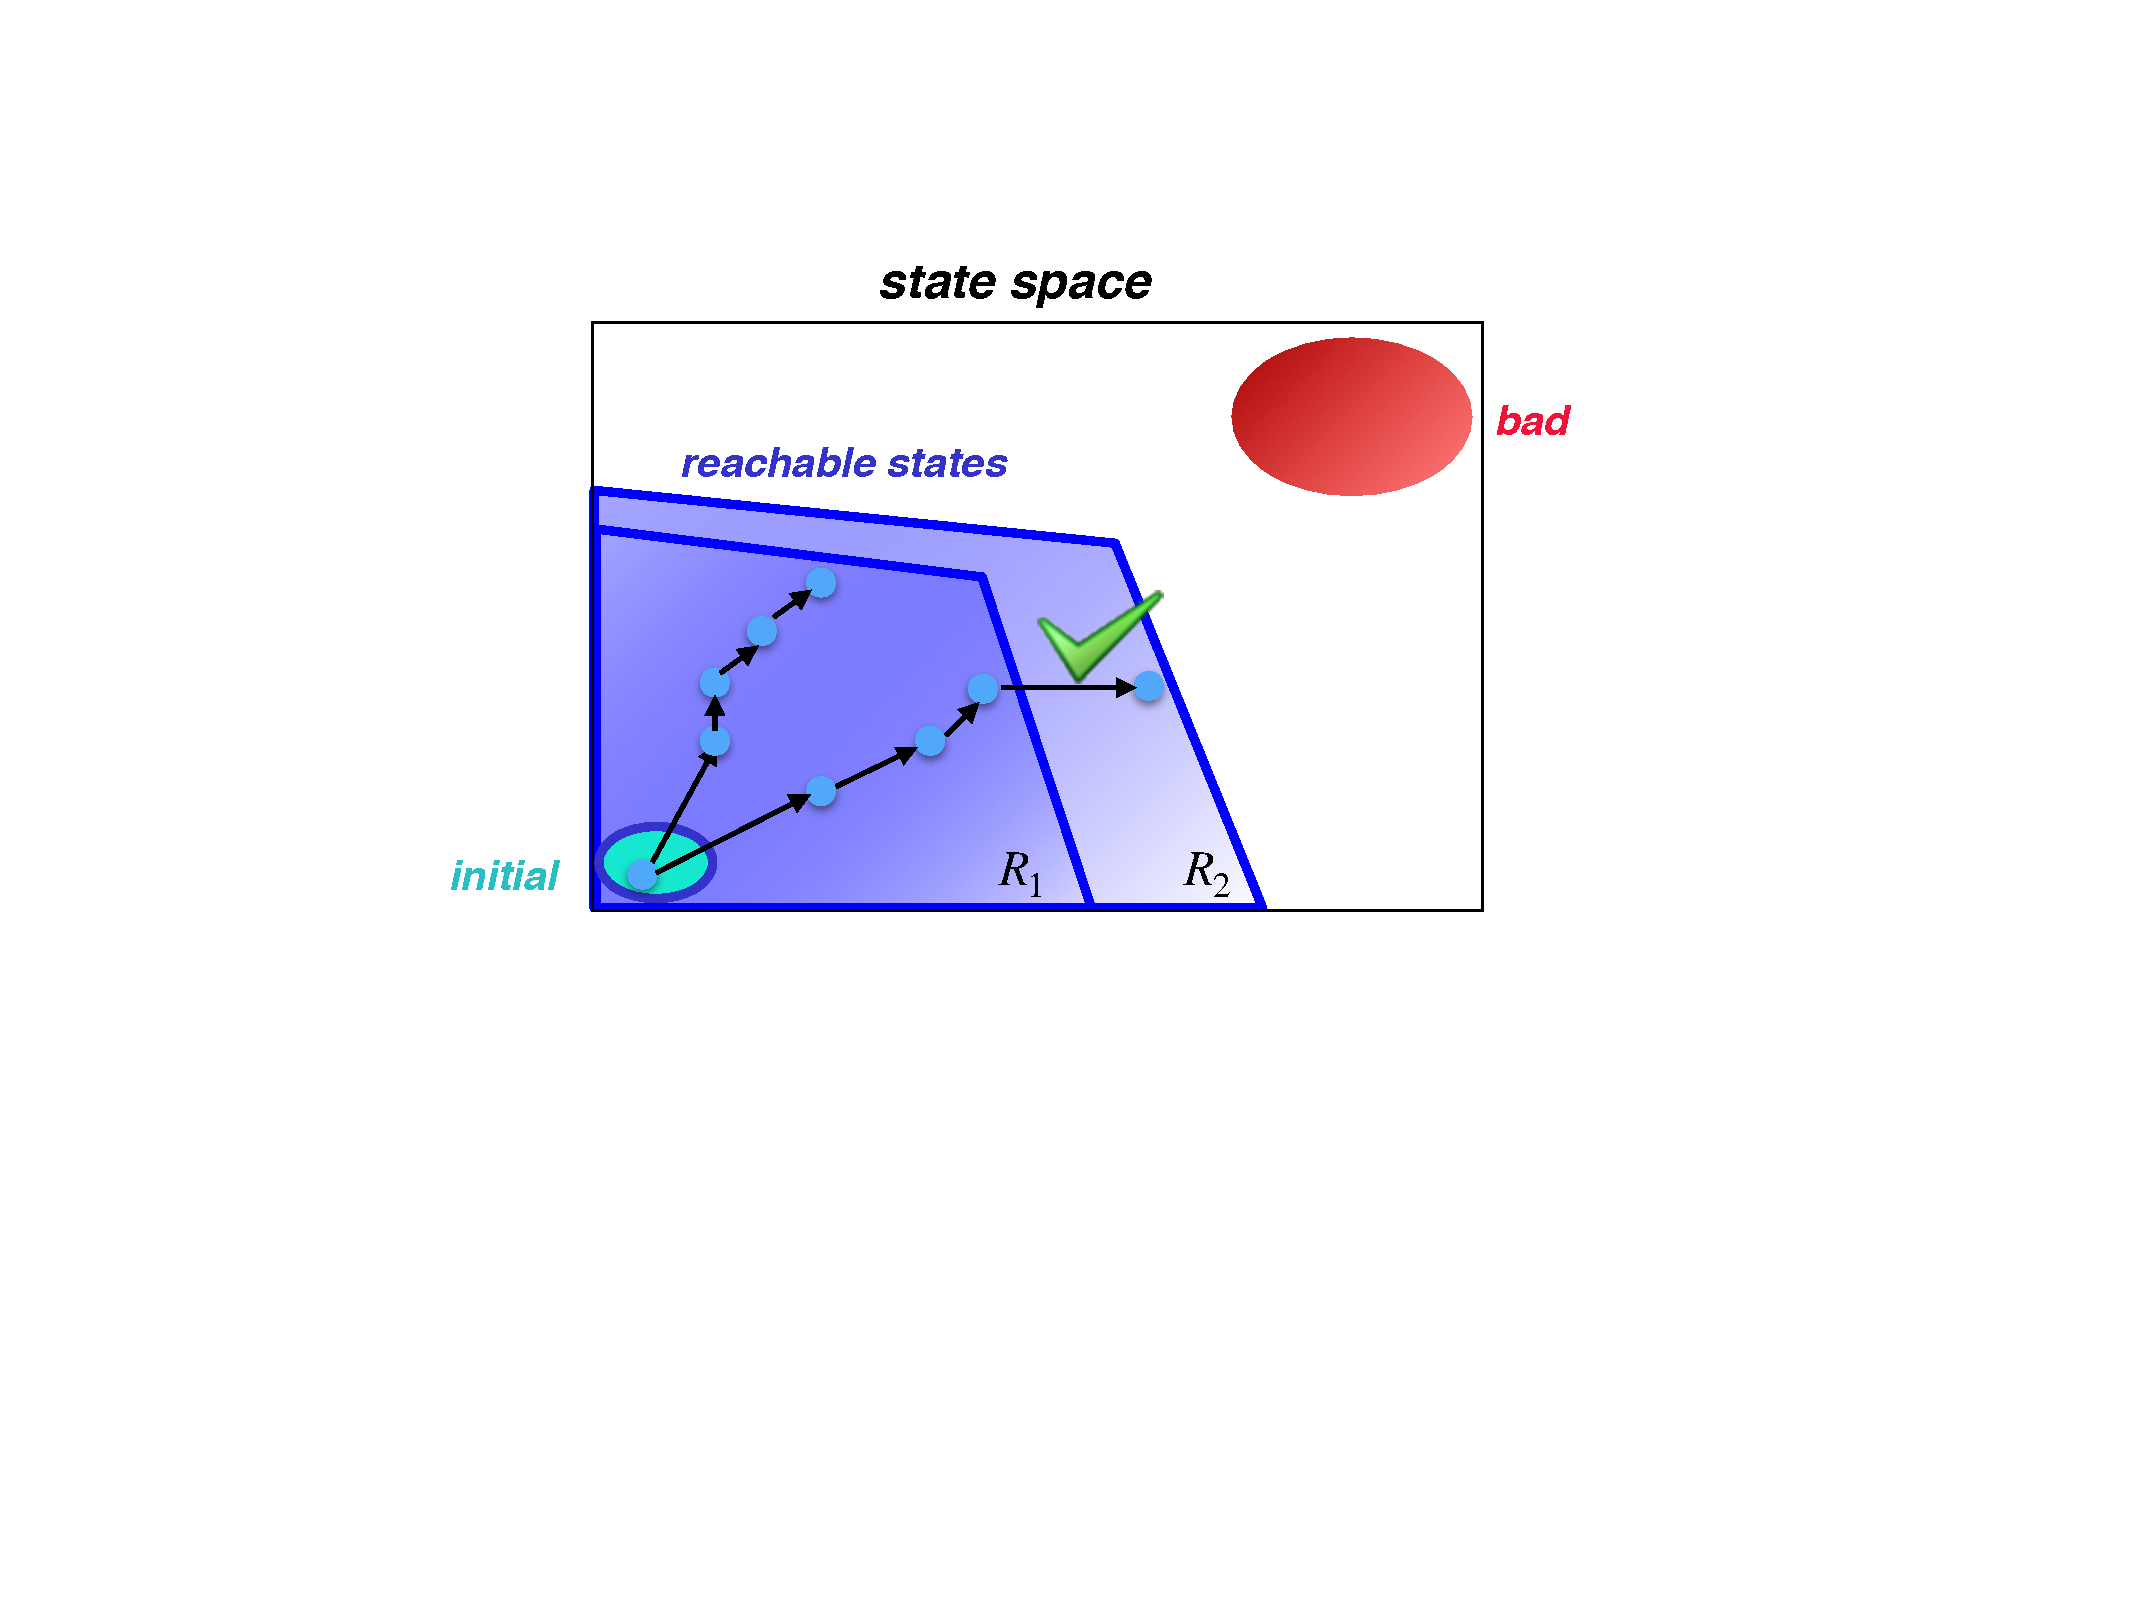
\includegraphics[width=0.5\textwidth]{figures/brain/reachability}
        \end{center}
    \end{block}
  }
  \only<2>{
    \begin{block}{\emph{Observation is ...}}
      {\bhand} \emph{$\reached[k]$ = the set of states reachable within $k$ contexts.}
    \end{block}
    \begin{block}{}
      \begin{center}
        \emph{$\reached[k]$ can be \alert{infinite}~[CAV'00],} \\
        \emph{but,} \\
        \emph{$\reached[k]$ can be \alert{finitely} represented~[TACAS'05].}
      \end{center}
    \end{block}
  }
\end{frame}
\begin{frame}
  \frametitle{(Un-)Decidability}
  \only<1>{
    \begin{block}{}
      \begin{center}
        {\color{blue}\ding{43}} {\it\bf Reachability of CPDS is \alert{undecidable}~[TOPLAS'00].}
      \end{center}
    \end{block}
    \begin{block}{\emph{But}}
      \begin{center}
        {\color{blue}\ding{43}} {\it\bf Context-\alert{bounded} reachability of CPDS is \alert{decidable}~[TACAS'05].}
      \end{center}
    \end{block}
  }
  % \only<2>{
  %   \begin{block}{\emph{Context-\alert{bounded} reachability of CPDS is \alert{decidable} because ...}}
  %     \vskip4pt
  %     {\bhand} \emph{$\reached[k]$ can be \alert{finitely} represented~[TACAS'05].}
  %   \end{block}
  % }
\end{frame}

\begin{frame}
  \frametitle{CUBA using Observation Sequences of Global States}
  \begin{block}{}
    {\bhand} \emph{$\OS := \reached[0], \reached[1],\reached[2], \ldots$, where each state in $\reached[k]$ is of the form:}
    \begin{center}
      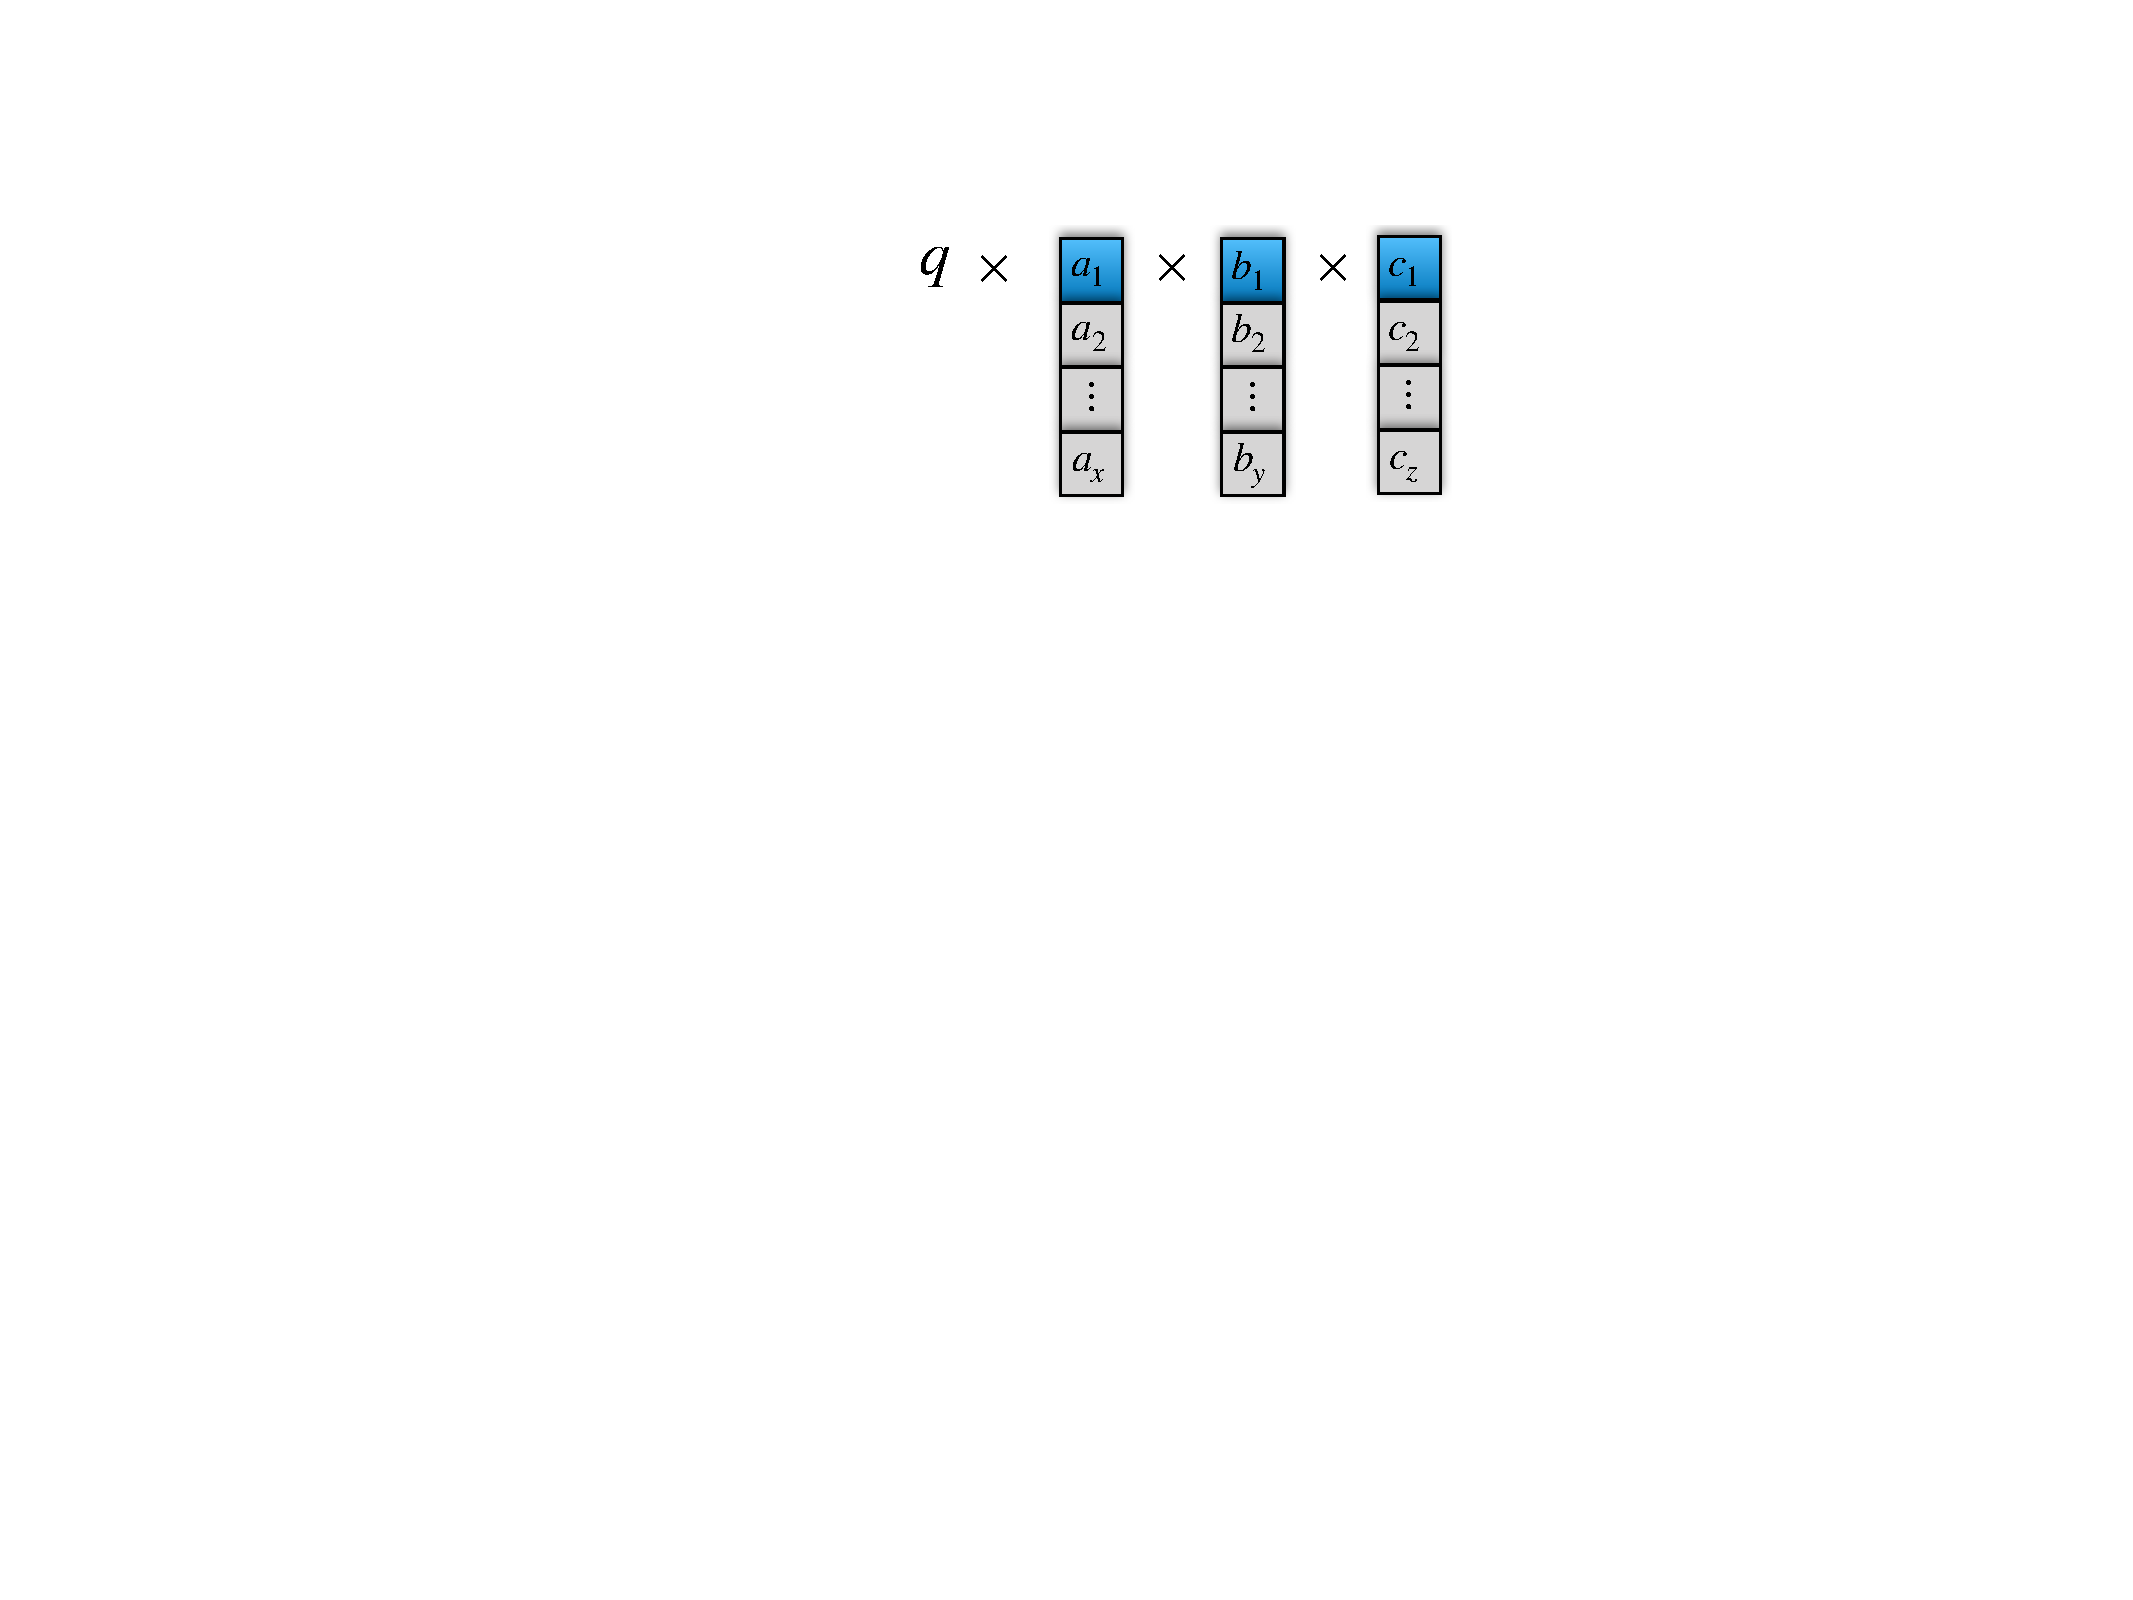
\includegraphics[width=0.3\textwidth]{figures/brain/cpds-state}
    \end{center}
    \vskip10pt
      \begin{center}
        \emph{$\OSone$ is defined over an \alert{infinite} domain and \alert{stutter-free}~[PLDI'18]}
      \end{center}
    \end{block}
\end{frame}

\begin{frame}
  \frametitle{Example}
  \only<1>{
    \begin{block}{}
      \vspace{-6pt}
      \begin{columns}
        \begin{column}{0.35\textwidth}
          \scriptsize{\hspace{6pt}\emph{Shared states:}}
          \[\scriptsize{
              \begin{array}{rl}
              \pdsshareds =& \{ \ 0, 1, 2, 3 \ \} \\[3em]

              \mbox{\emph{Thread 1:}} & \\
              \alphabet_1 = & \{ \ 1, 2 \ \} \\
              \pdstranss_{1} = &                  \{ \ f_1:     \threadstate 0 1  \pdstranssymbol \threadstate 1 2 \ , \\
                            & \pos[r]{$f_2:$}{$\{ \ f_1:$} \ \threadstate 3 2  \pdstranssymbol \threadstate 0 1 \ \} \\[3em]

              \mbox{\emph{Thread 2:}} & \\
              \alphabet_2 = & \{ \ 4, 5, 6 \ \}\\
              \pdstranss_{2} = &                  \{ \ b_1:     \threadstate 0 4  \pdstranssymbol \threadstate 0 {\emptystack} \ , \\
                          & \pos[r]{$b_2:$}{$\{ \ b_1:$} \ \threadstate 1 4  \pdstranssymbol \threadstate 2 5 \ , \\
                          & \pos[r]{$b_3:$}{$\{ \ b_3:$} \ \threadstate 2 5  \pdstranssymbol \threadstate 3 {4 6} \ \} \\[3em]
              \pdsinitstate = & 0
            \end{array}}\]
        \end{column}
        \begin{column}{.65\textwidth}
          \begin{minipage}{.75\textwidth}
  \centering
  \resizebox{.9\textwidth}{!}{
    \begin{tikzpicture}[->,>=stealth',shorten >=1pt,auto,node distance=2.0cm, semithick, 
      state/.style={minimum size=14pt,inner sep=-0.1pt,font=\small\rmfamily},
      round/.style = {rounded corners=1.5mm,dashed }, font=\sffamily]
      \tikzstyle{every state}=[minimum size=1mm]
      \tikzstyle{selected} = [draw,line width=5pt,-,gray!60]
      \begin{scope}[xshift=0cm,yshift=5cm]
        \draw[round] (-5.0,0.50) rectangle (3.0,-0.5);
        \node[] at (-4.6,-0.3) {$R_0$};
        \draw[round] (-5.1,0.55) rectangle (3.1,-2.0);
        \node[] at (-4.7,-1.8) {$R_1$};
        \draw[round] (-5.2,0.60) rectangle (3.2,-3.5);
        \node[] at (-4.8,-3.3) {$R_2$};
        \draw[round] (-5.3,0.65) rectangle (3.3,-5.0);
        \node[] at (-4.9,-4.8) {$R_3$};
        \draw[round] (-5.4,0.70) rectangle (3.4,-6.5);
        \node[] at (-5.0,-6.3) {$R_4$};
        \draw[round] (-5.5,0.75) rectangle (3.5,-8.0);
        \node[] at (-5.1,-7.8) {$R_5$};
        \draw[round] (-5.6,0.80) rectangle (3.6,-9.5);
        \node[] at (-5.2,-9.3) {$R_6$};
        \draw[round] (-5.7,0.85) rectangle (3.7,-10.0);
        \node[] at (-1.0,-9.8) {\bf ......};

        % k = 0
        \node[state] (014) {$\config 0 {1,4}$};
        % k = 1
        \node[state] (124) [below left of  = 014] {$\config 1 {2,4}$};
        \node[state] (01e) [below right of = 014] {$\config 0 {1,\emptyword}$};
        % k = 2
        \node[state] (225) [below = 1cm of 124] {$\config 2 {2,5}$};
        \node[state] (12e) [below = 1cm of 01e] {$\config 1 {2,\emptyword}$};
        \node[state] (3246) [left of  = 225] {$\config 3 {2,46}$};
        % k = 3
        \node[state] (0146) [below = 1cm of 3246] {$\config 0 {1,46}$};
        \node[state] (1246) [right of  = 0146] {$\config 1 {2,46}$};
        % k = 4
        \node[state] (016) [below = 1cm of 0146] {$\config 0 {1,6}$};
        \node[state] (2256) [right of  = 016] {$\config 2 {2,56}$};
        \node[state] (32466) [right = 1.2cm of 2256] {$\config 3 {2,466}$};
        % k = 5
        \node[state] (01466) [below = 1cm of 32466] {$\config 0 {1,466}$};
        \node[state] (12466) [left = 1.0cm of 01466] {$\config 1 {2,466}$};
        \node[state] (126) [below = 1cm of 016] {$\config 1 {2,6}$};
        % k = 6
        \node[state] (0166)  [below = 1cm of 01466] {$\config 0 {1,66}$};
        \node[state] (22566) [below = 1cm of 12466] {$\config 2 {2,566}$};
        \node[state] (324666) [below = 1cm of 126] {$\config 3 {2,4666}$};


        \draw [selected] (0146) -- (016);
        \path[]
        (014)  edge[left]     node {\scriptsize $f_1$} (124)
        (014)  edge[right]     node {\scriptsize $b_1$} (01e)
        (124)  edge[left]      node {\scriptsize $b_2$} (225)
        (01e)  edge[right]     node {\scriptsize $f_1$} (12e)
        (225)  edge[above]     node {\scriptsize $b_3$} (3246)
        (3246) edge[left]      node {\scriptsize $f_2$} (0146)
        (0146) edge[above]     node {\scriptsize $f_1$} (1246)
        (0146) edge[left]      node {\scriptsize $b_1$} (016)
        (1246) edge[right]     node {\scriptsize $b_2$} (2256)
        (2256) edge[above]     node {\scriptsize $b_3$} (32466)
        (32466)edge[right]     node {\scriptsize $f_2$} (01466)
        (01466)edge[above]     node {\scriptsize $f_1$} (12466)
        (016)  edge[left]      node {\scriptsize $f_1$} (126)
        (12466)edge[left]      node {\scriptsize $b_2$} (22566)
        (22566)edge[above]     node {\scriptsize $b_3$} (324666)
        (01466)edge[left]      node {\scriptsize $b_1$} (0166);
        
        % \path[->] (324666) edge[color=red,bend left]  (32466);
        % \path[->] (0166) edge[color=red,bend right]  (016);
        % \path[->] (22566) edge[color=red,bend left]  (2256);

        % \node[cloud,draw,color=red] (diverge) [right = 2.6cm of 01e] {diverge};
      \end{scope}
    \end{tikzpicture}}
\end{minipage}

        \end{column}
      \end{columns}
    \end{block}}
  \only<2>{
    \begin{block}{}
      \vspace{-6pt}
      \begin{columns}
        \begin{column}{0.35\textwidth}
          \scriptsize{\hspace{6pt}\emph{Shared states:}}
          \[\scriptsize{
              \begin{array}{rl}
              \pdsshareds =& \{ \ 0, 1, 2, 3 \ \} \\[3em]

              \mbox{\emph{Thread 1:}} & \\
              \alphabet_1 = & \{ \ 1, 2 \ \} \\
              \pdstranss_{1} = &                  \{ \ f_1:     \threadstate 0 1  \pdstranssymbol \threadstate 1 2 \ , \\
                            & \pos[r]{$f_2:$}{$\{ \ f_1:$} \ \threadstate 3 2  \pdstranssymbol \threadstate 0 1 \ \} \\[3em]

              \mbox{\emph{Thread 2:}} & \\
              \alphabet_2 = & \{ \ 4, 5, 6 \ \}\\
              \pdstranss_{2} = &                  \{ \ b_1:     \threadstate 0 4  \pdstranssymbol \threadstate 0 {\emptystack} \ , \\
                          & \pos[r]{$b_2:$}{$\{ \ b_1:$} \ \threadstate 1 4  \pdstranssymbol \threadstate 2 5 \ , \\
                          & \pos[r]{$b_3:$}{$\{ \ b_3:$} \ \threadstate 2 5  \pdstranssymbol \threadstate 3 {4 6} \ \} \\[3em]
              \pdsinitstate = & 0
            \end{array}}\]
        \end{column}
        \begin{column}{.75\textwidth}
          \centering
          \begin{minipage}{.75\textwidth}
  \centering
  \resizebox{1.05\textwidth}{!}{
    \begin{tikzpicture}[->,>=stealth',shorten >=1pt,auto,node distance=2.0cm, semithick, 
      state/.style={minimum size=14pt,inner sep=-0.1pt,font=\small\rmfamily},
      round/.style = {rounded corners=1.5mm,dashed }, font=\sffamily]
      \tikzstyle{every state}=[minimum size=1mm]
      \tikzstyle{selected} = [draw,line width=5pt,-,gray!60]
      \begin{scope}[xshift=0cm,yshift=5cm]
        \draw[round] (-5.0,0.50) rectangle (3.0,-0.5);
        \node[] at (-4.6,-0.3) {$R_0$};
        \draw[round] (-5.1,0.55) rectangle (3.1,-2.0);
        \node[] at (-4.7,-1.8) {$R_1$};
        \draw[round] (-5.2,0.60) rectangle (3.2,-3.5);
        \node[] at (-4.8,-3.3) {$R_2$};
        \draw[round] (-5.3,0.65) rectangle (3.3,-5.0);
        \node[] at (-4.9,-4.8) {$R_3$};
        \draw[round] (-5.4,0.70) rectangle (3.4,-6.5);
        \node[] at (-5.0,-6.3) {$R_4$};
        \draw[round] (-5.5,0.75) rectangle (3.5,-8.0);
        \node[] at (-5.1,-7.8) {$R_5$};
        \draw[round] (-5.6,0.80) rectangle (3.6,-9.5);
        \node[] at (-5.2,-9.3) {$R_6$};
        \draw[round] (-5.7,0.85) rectangle (3.7,-10.0);
        \node[] at (-1.0,-9.8) {\bf ......};

        % k = 0
        \node[state] (014) {$\config 0 {1,4}$};
        % k = 1
        \node[state] (124) [below left of  = 014] {$\config 1 {2,4}$};
        \node[state] (01e) [below right of = 014] {$\config 0 {1,\emptyword}$};
        % k = 2
        \node[state] (225) [below = 1cm of 124] {$\config 2 {2,5}$};
        \node[state] (12e) [below = 1cm of 01e] {$\config 1 {2,\emptyword}$};
        \node[state] (3246) [left of  = 225] {$\config 3 {2,46}$};
        % k = 3
        \node[state] (0146) [below = 1cm of 3246] {$\config 0 {1,46}$};
        \node[state] (1246) [right of  = 0146] {$\config 1 {2,46}$};
        % k = 4
        \node[state] (016) [below = 1cm of 0146] {$\config 0 {1,6}$};
        \node[state] (2256) [right of  = 016] {$\config 2 {2,56}$};
        \node[state] (32466) [right = 1.2cm of 2256] {$\config 3 {2,466}$};
        % k = 5
        \node[state] (01466) [below = 1cm of 32466] {$\config 0 {1,466}$};
        \node[state] (12466) [left = 1.0cm of 01466] {$\config 1 {2,466}$};
        \node[state] (126) [below = 1cm of 016] {$\config 1 {2,6}$};
        % k = 6
        \node[state] (0166)  [below = 1cm of 01466] {$\config 0 {1,66}$};
        \node[state] (22566) [below = 1cm of 12466] {$\config 2 {2,566}$};
        \node[state] (324666) [below = 1cm of 126] {$\config 3 {2,4666}$};


        \draw [selected] (0146) -- (016);
        \path[]
        (014)  edge[left]     node {\scriptsize $f_1$} (124)
        (014)  edge[right]     node {\scriptsize $b_1$} (01e)
        (124)  edge[left]      node {\scriptsize $b_2$} (225)
        (01e)  edge[right]     node {\scriptsize $f_1$} (12e)
        (225)  edge[above]     node {\scriptsize $b_3$} (3246)
        (3246) edge[left]      node {\scriptsize $f_2$} (0146)
        (0146) edge[above]     node {\scriptsize $f_1$} (1246)
        (0146) edge[left]      node {\scriptsize $b_1$} (016)
        (1246) edge[right]     node {\scriptsize $b_2$} (2256)
        (2256) edge[above]     node {\scriptsize $b_3$} (32466)
        (32466)edge[right]     node {\scriptsize $f_2$} (01466)
        (01466)edge[above]     node {\scriptsize $f_1$} (12466)
        (016)  edge[left]      node {\scriptsize $f_1$} (126)
        (12466)edge[left]      node {\scriptsize $b_2$} (22566)
        (22566)edge[above]     node {\scriptsize $b_3$} (324666)
        (01466)edge[left]      node {\scriptsize $b_1$} (0166);
        
        \path[->] (324666) edge[color=red,bend left]  (32466);
        \path[->] (0166) edge[color=red,bend right]  (016);
        \path[->] (22566) edge[color=red,bend left]  (2256);

        \node[circle, draw, color=red, inner sep=2pt, minimum size=1pt] (c1) [below right = 0.6cm of 0166] {};
        \node[circle, draw, color=red,inner sep=3pt,minimum size=1pt](c2) [above right = 0.5cm of c1] {};
        \node[circle, draw, color=red,inner sep=4pt,minimum size=1pt](c3) [above right = 0.5cm of c2] {};
        % \node[circle, draw, color=red,inner sep=5pt,minimum size=1pt](c4) [above right = 0.5cm of c3] {};

        \node[cloud,draw,color=red] (diverge) [above right = 0.6cm of c3] {\emph{diverge}};
      \end{scope}
    \end{tikzpicture}}
\end{minipage}

        \end{column}
      \end{columns}
    \end{block}
  }
\end{frame}

\begin{frame}
  \frametitle{How to Proceed?}
  \begin{block}<1->{\emph{Give up?}}
    \vskip4pt
    % \emph{If your conjecture is not true, find assumptions under which it is true.}\linebreak
    % \begin{flushright}
    %   \textbf{-- XXXX}
    % \end{flushright}
  \end{block}
  \begin{block}<2>{\emph{Well, do not give up so quickly. Because we know ...}}
  \end{block}
  \begin{block}<2>{\emph{Convergence Property}}
    \vskip4pt
    \begin{center}
      \emph{An OS $\OS$ over a \alert{finite} domain always converges.}
    \end{center}
  \end{block}
\end{frame}

\begin{frame}
  \frametitle{CUBA using Observation Sequences of Visible State}
  \only<1>{
    \begin{block}{\emph{Project global states to a finite domain ...}}
      \vskip4pt
      {\color{blue}\ding{43}} \emph{by cutting off tails of stacks.}
    \end{block}
    \begin{block}{}%{\emph{Vividly}}
        \begin{center}
          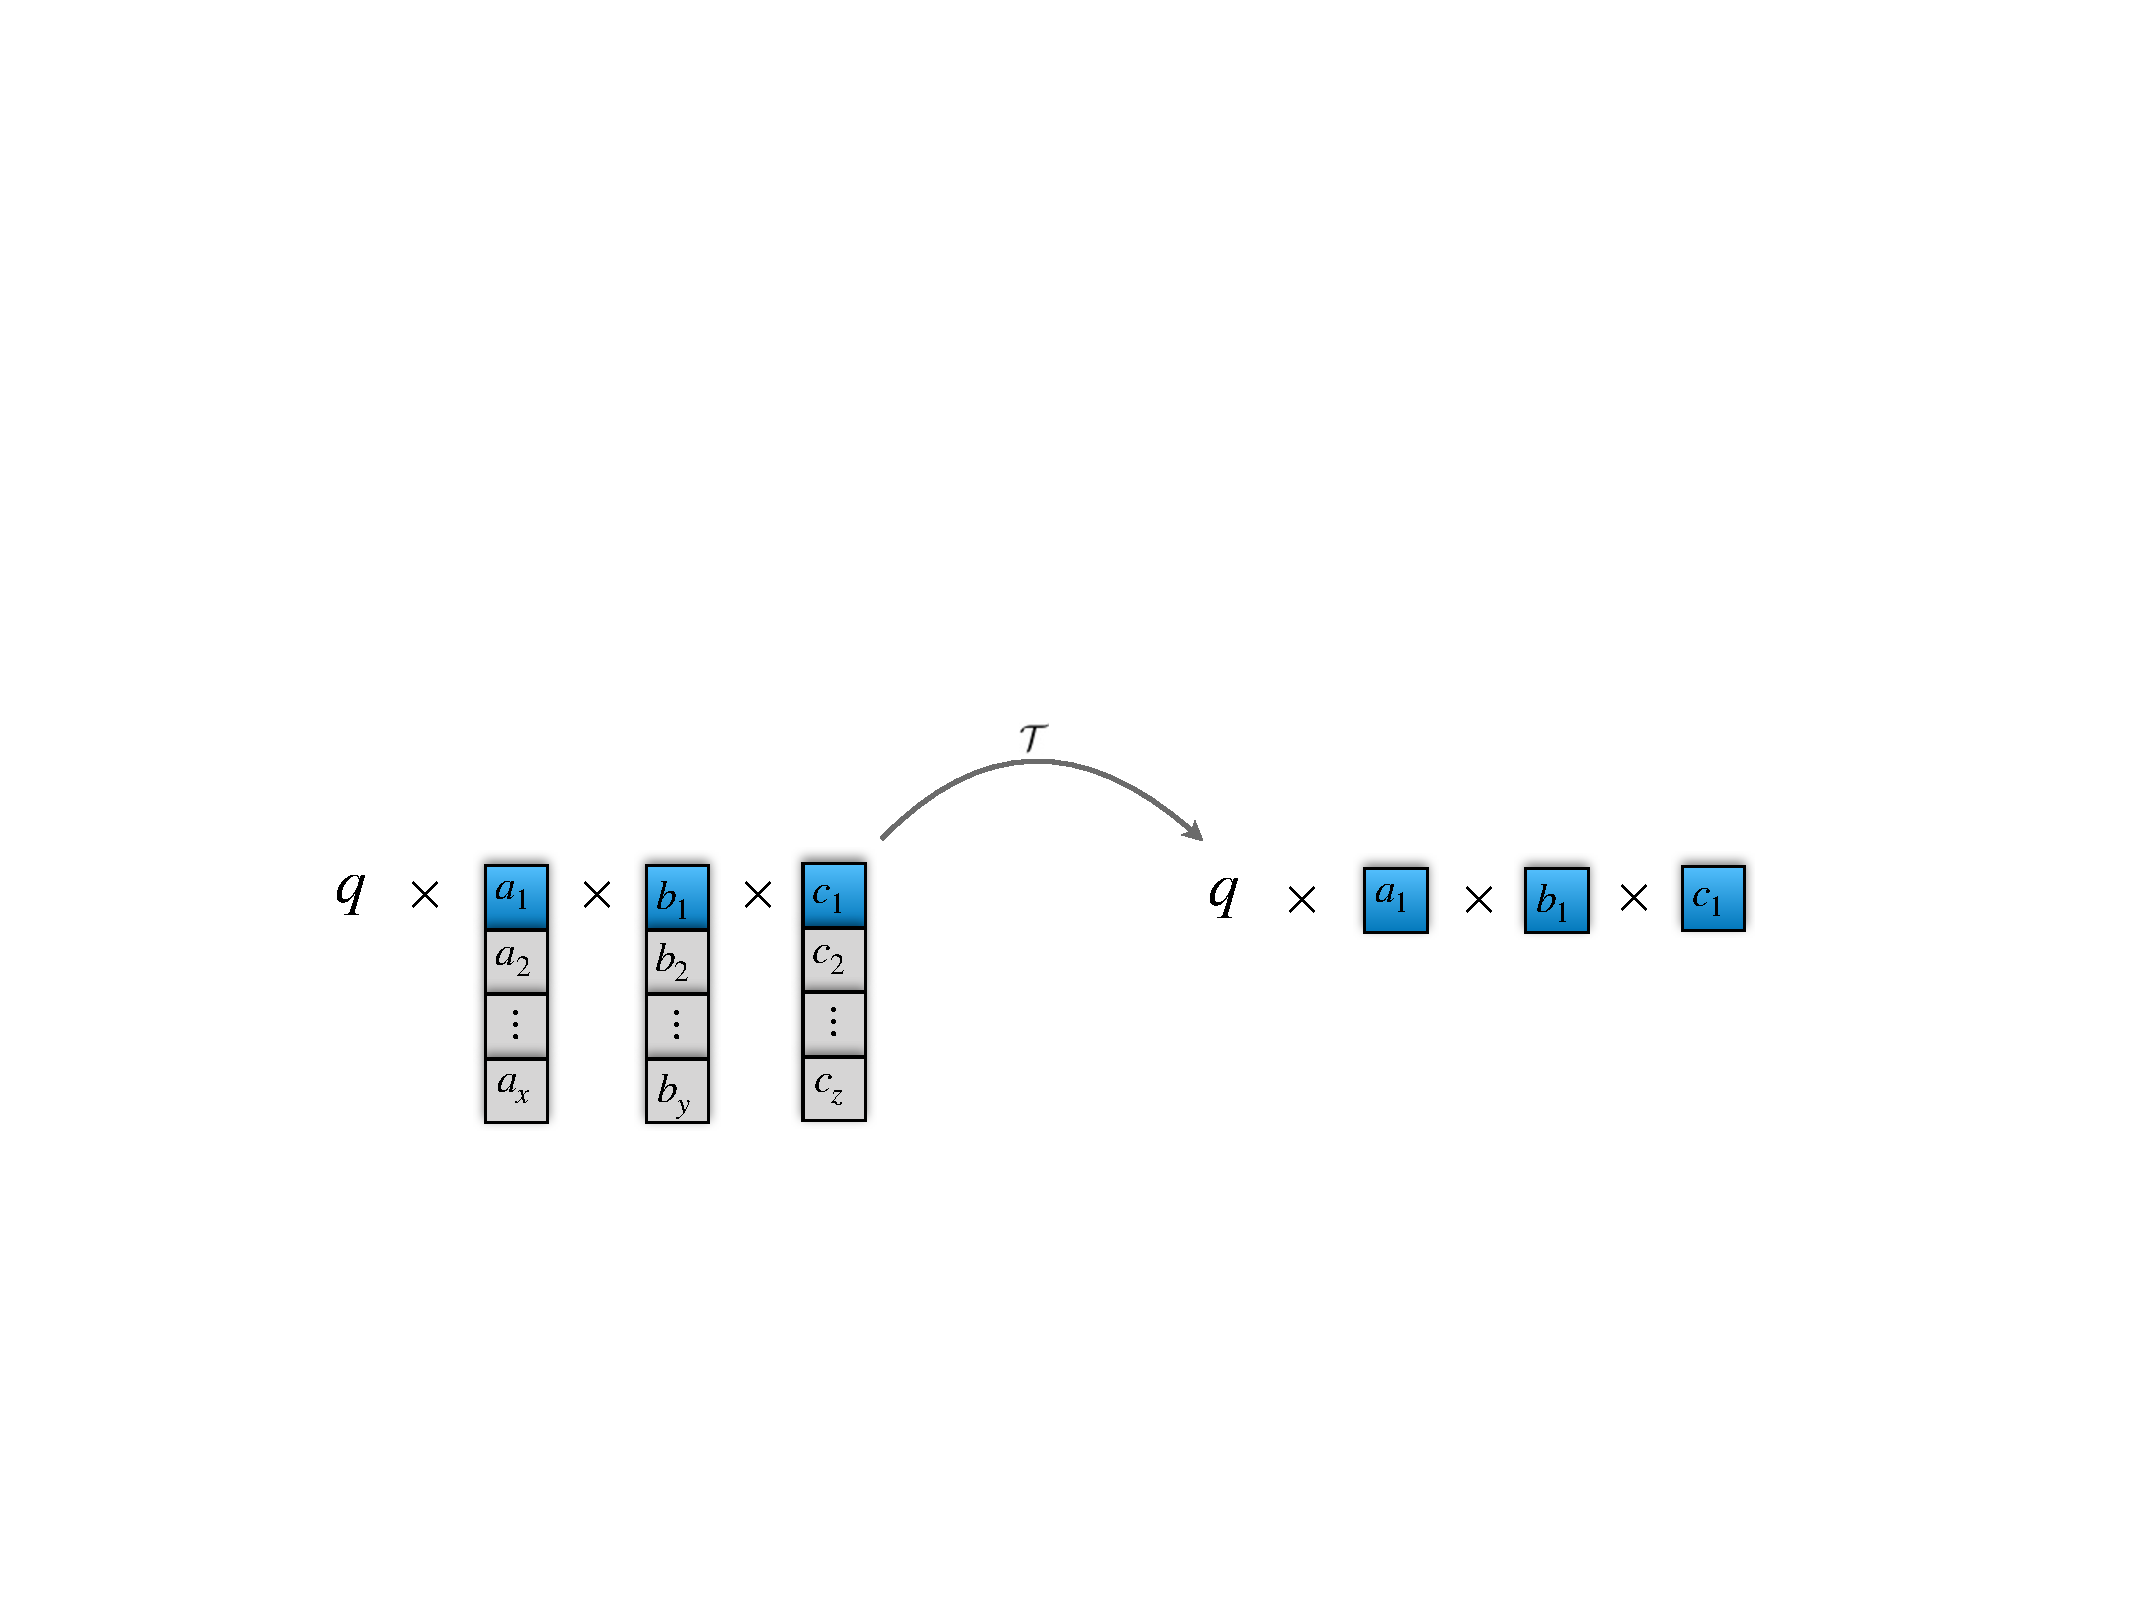
\includegraphics[width=0.9\textwidth]{figures/brain/topping}
        \end{center}
    \end{block}
  }

  \only<2>{
    \begin{block}{\emph{Project global states to a finite domain ...}}
      \vskip4pt
    \begin{center}
      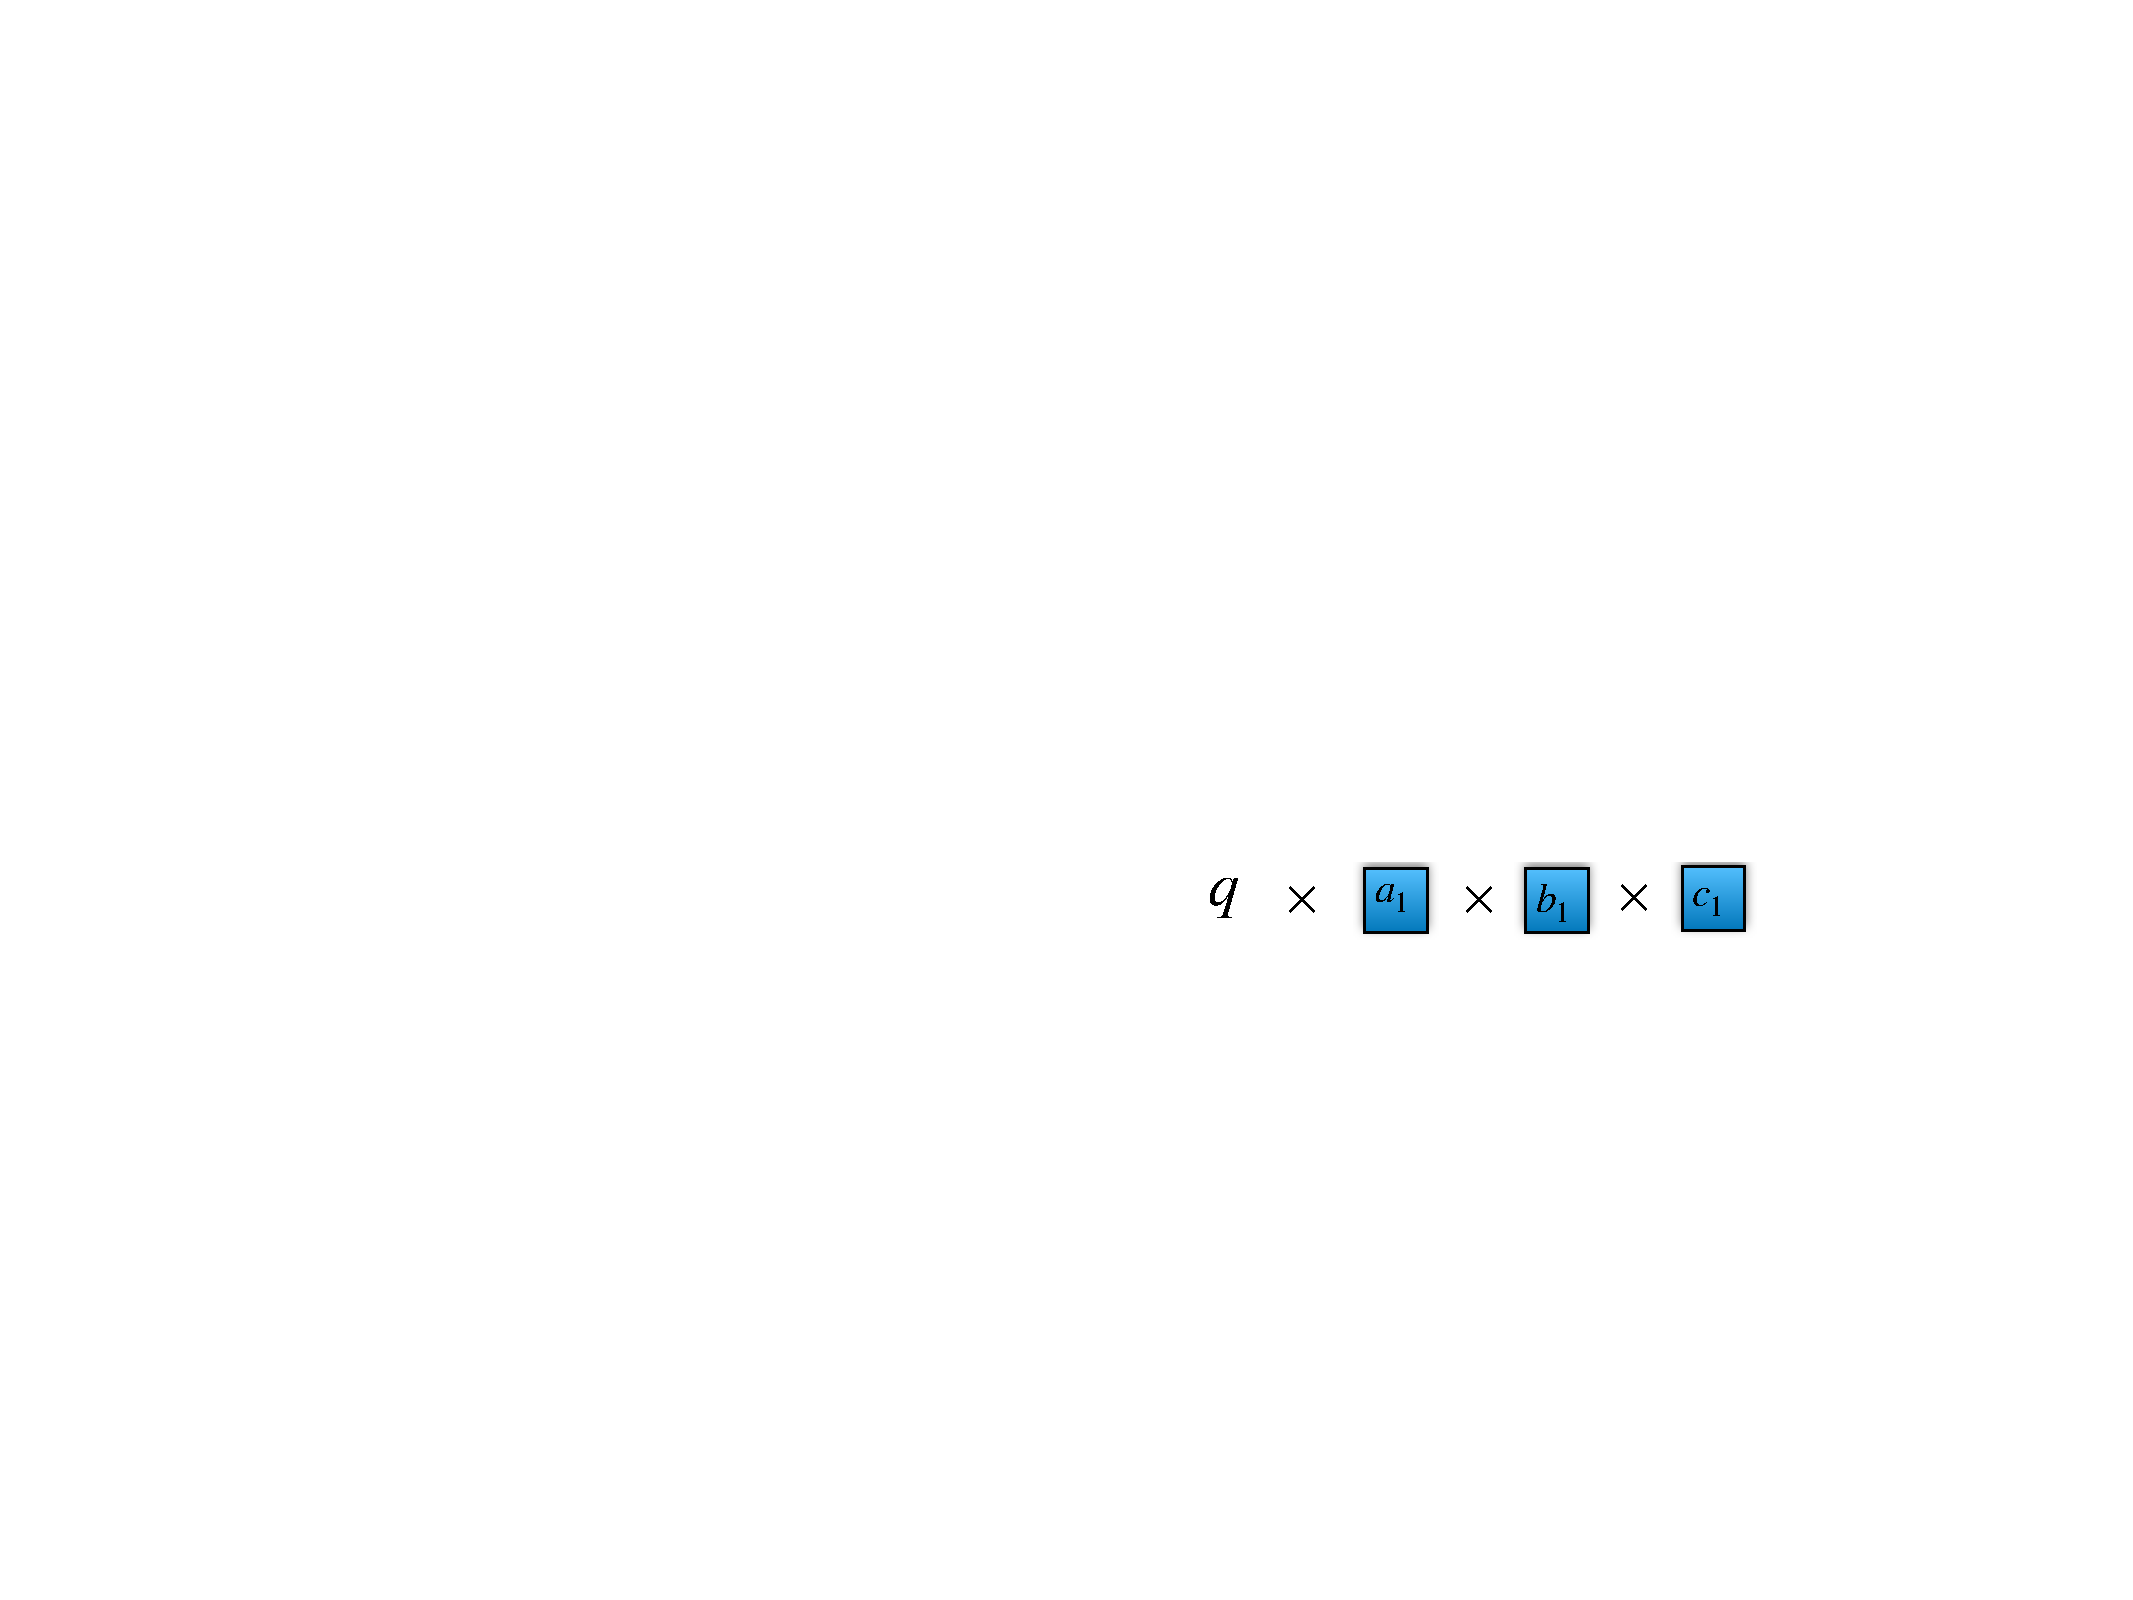
\includegraphics[width=0.3\textwidth]{figures/brain/visible-state}
    \end{center}
    \end{block}
    \begin{block}{\emph{Visible states}}
      \begin{enumerate}[\bhand]
        \item \emph{suffice to express many safety properties, e.g. various assertions, data race, race condition, etc}.
      \end{enumerate}
    \end{block}}

  \only<3>{
  \begin{block}{}
    {\bhand} \emph{$\OS := \visible[0], \visible[1],\visible[2], \ldots$, where each state in $\visible[k]$ is of the form:}
    \begin{center}
      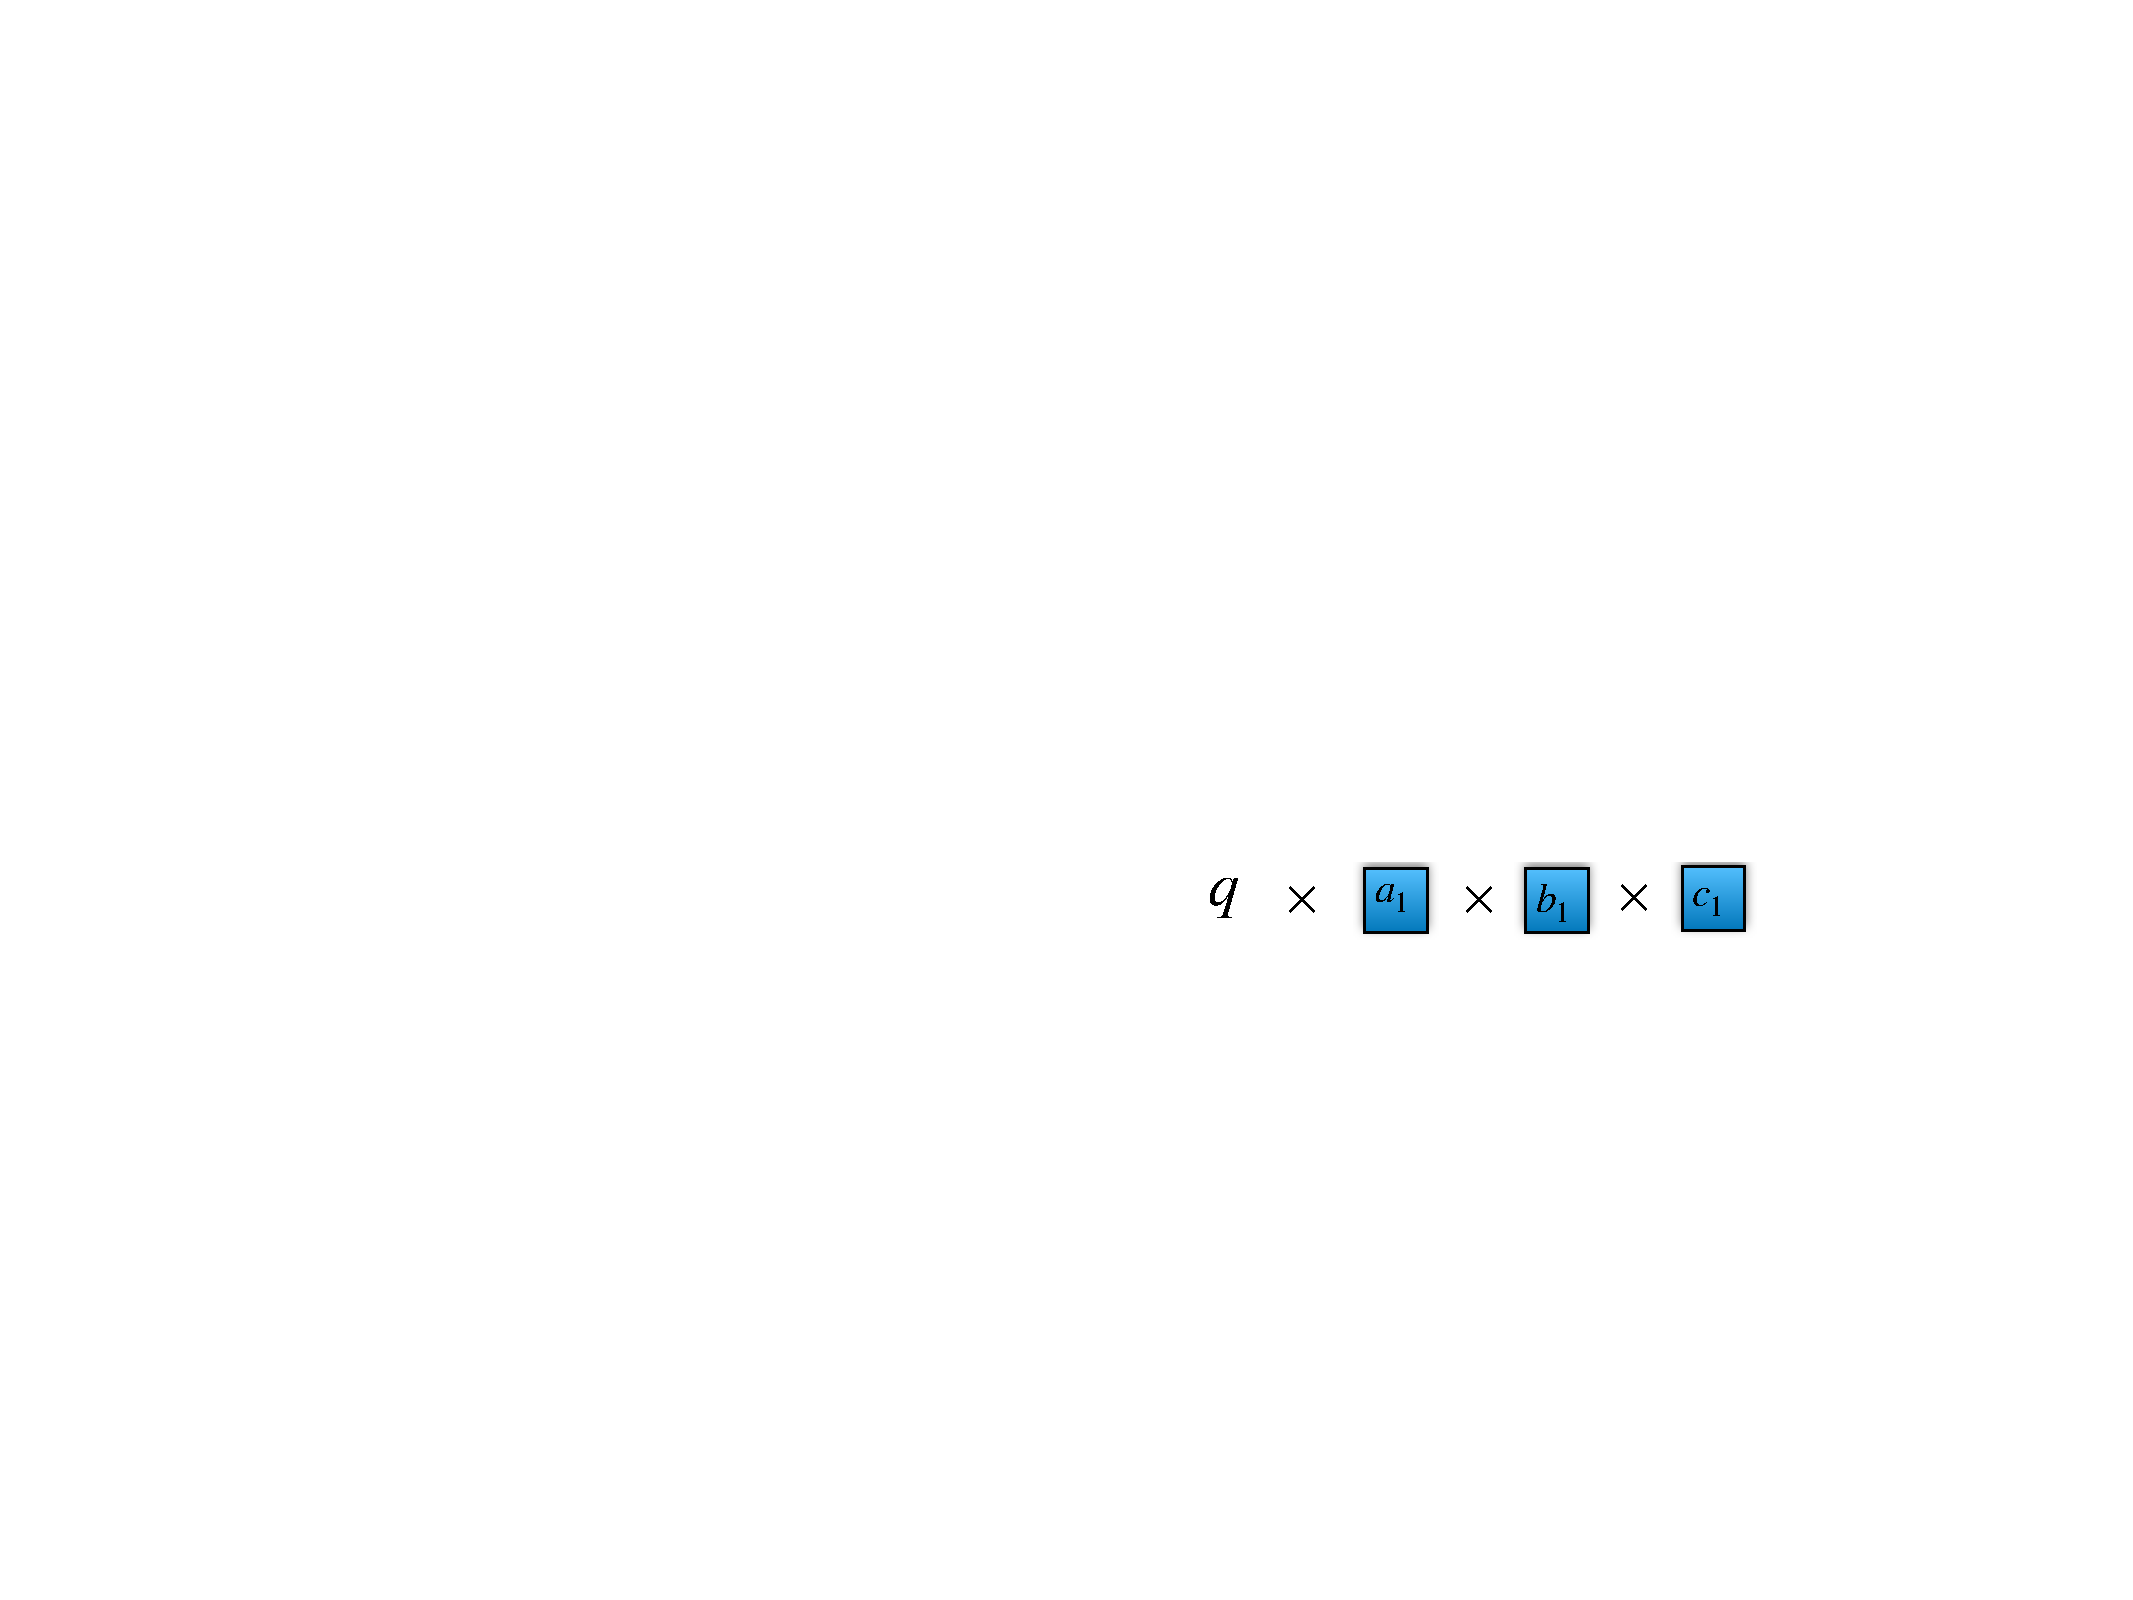
\includegraphics[width=0.3\textwidth]{figures/brain/visible-state}
    \end{center}
    \vskip10pt
      \begin{center}
        \emph{$\OSthree$ is guaranteed to \alert{converge}.}\\
        \[
          \visible[k] := \topmap{\reached[k]}
          \]
      \end{center}
    \end{block}}
\end{frame}

\begin{frame}
  \frametitle{Example Revisited}
  \only<1>{
    \begin{block}{\emph{\scriptsize{Can we answer the convergence of visible state sequence easily?}}}
      \vspace{0pt}
      \begin{columns}
        \begin{column}{1\textwidth}
          % \documentclass[preview, landscape]{standalone}

% \usepackage{pgf}
% \usepackage{tikz}
% \usetikzlibrary{arrows,positioning}

% \newcommand{\config}[2]{\langle{#1\!\mid\!#2}\rangle} % compare typesetting: $q|x,y$ vs $q\mid x,y$ vs $q\!\mid\!x,y$
% \newcommand{\emptyword}  {\varepsilon}

% \usepackage{bbm}
% \usepackage{dsfont}
% \begin{document}
% \centerTwoOut{

% \begin{minipage}{.20\textwidth}
%   \[
%     \begin{array}{lll}
%       \pdsshareds & = & \{ \ 0, 1, 2, 3 \ \} \\[1em]

%       \alphabet_1 & = & \{ \ 1, 2 \ \} \\
%       \alphabet_2 & = & \{ \ 4, 5, 6 \ \}\\[1em]

%       \pdstranss_{1} & = &                  \{ \ f_1:     \threadstate 0 1  \pdstranssymbol \threadstate 1 2 \ , \\
%                      &   & \pos[r]{$f_2:$}{$\{ \ f_1:$} \ \threadstate 3 2  \pdstranssymbol \threadstate 0 1 \ \} \\[1em]
%       \pdstranss_{2} & = &                  \{ \ b_1:     \threadstate 0 4  \pdstranssymbol \threadstate 0 {\emptystack} \ , \\
%                      &   & \pos[r]{$b_2:$}{$\{ \ b_1:$} \ \threadstate 1 4  \pdstranssymbol \threadstate 2 5 \ , \\
%                      &   & \pos[r]{$b_3:$}{$\{ \ b_3:$} \ \threadstate 2 5  \pdstranssymbol \threadstate 3 {4 6} \ \} \\[1em]
%       \pdsinitstate  & = & 0
%     \end{array}
%   \]
%   % initial state:
%   % \[
%   %   \config 0 {1,4}
%   % \]
% \end{minipage}
% \hfill
\begin{minipage}{.8\textwidth}
  \centering
  \resizebox{.90\textwidth}{!}{
    \begin{tikzpicture}[->,>=stealth',shorten >=1pt,auto,node distance=2.0cm, semithick, 
      state/.style={minimum size=14pt,inner sep=-0.1pt,font=\small\rmfamily},
      round/.style = {rounded corners=1.5mm,dashed }, font=\sffamily]
      \tikzstyle{every state}=[minimum size=1mm]
      \tikzstyle{selected} = [draw,line width=5pt,-,gray!60]
      \begin{scope}[xshift=0cm,yshift=5cm]
        \draw[round] (-5.0,0.50) rectangle (3.0,-0.5);
        \node[] at (-4.6,-0.3) {$R_0$};
        \draw[round] (-5.1,0.55) rectangle (3.1,-2.0);
        \node[] at (-4.7,-1.8) {$R_1$};
        \draw[round] (-5.2,0.60) rectangle (3.2,-3.5);
        \node[] at (-4.8,-3.3) {$R_2$};
        \draw[round] (-5.3,0.65) rectangle (3.3,-5.0);
        \node[] at (-4.9,-4.8) {$R_3$};
        \draw[round] (-5.4,0.70) rectangle (3.4,-6.5);
        \node[] at (-5.0,-6.3) {$R_4$};
        \draw[round] (-5.5,0.75) rectangle (3.5,-8.0);
        \node[] at (-5.1,-7.8) {$R_5$};
        \draw[round] (-5.6,0.80) rectangle (3.6,-9.5);
        \node[] at (-5.2,-9.3) {$R_6$};
        \draw[round] (-5.7,0.85) rectangle (3.7,-10.0);
        \node[] at (-1.0,-9.8) {\bf ......};

        \draw[round] (6.0,0.50) rectangle (10.0,-0.5);
        \node[] at (6.3,-0.3) {$\visible[0]$};
        \draw[round] (5.9,0.55) rectangle (10.1,-2.0);
        \node[] at (6.2,-1.8) {$\visible[1]$};
        \draw[round] (5.8,0.60) rectangle (10.2,-3.5);
        \node[] at (6.1,-3.3) {$\visible[2]$};
        \draw[round,name=B] (5.7,0.65) rectangle (10.3,-5.0);
        \node[] at (6.0,-4.8) {$\visible[3]$};
        \draw[round] (5.6,0.70) rectangle (10.4,-6.5);
        \node[] at (5.9,-6.3) {$\visible[4]$};
        \draw[round] (5.5,0.75) rectangle (10.5,-8.0);
        \node[] at (5.8,-7.8) {$\visible[5]$};
        \draw[round] (5.4,0.80) rectangle (10.6,-9.5);
        \node[] at (5.7,-9.3) {$\visible[6]$};
        \draw[round] (5.3,0.85) rectangle (10.7,-10.0);
        \node[] at (8.1,-9.8) {\bf ......};

        \node[](1) at (8.0,0.0) {$\config 0 {1,4}$};
        \node[](2)[below =0.3cm of 1] {$\config 1 {2,4}$};
        \node[](3)[below =0.1cm of 2] {$\config 0 {1,\emptyword}$};
        \node[](4)[below =0.0cm of 3] {$\config 2 {2,5}$};
        \node[](5)[below left  = -0.5mm of 4] {$\config 3 {2,4}$};
        \node[](6)[below right = -0.5mm of 4] {$\config 1 {2,\emptyword}$};
        \node[](7) at (8.0,-5.8) {$\config 0 {1,6}$};
        \node[](8) [below = 0.7cm of 7] {$\config 1 {2,6}$};
        \draw[->, >=latex', shorten >=2pt, bend left=45, thick, dashed] 
        (2.9,0.3) to node[auto, swap] {$\mathcal T$}(6.1,0.3); 
        \draw[->, >=latex', shorten >=2pt, bend left=45, thick, dashed] 
        (3.0,-1.2) to node[auto, swap] {$\mathcal T$}(6.0,-1.2);
        \draw[->, >=latex', shorten >=2pt, bend left=45, thick, dashed] 
        (3.1,-2.7) to node[auto, swap] {$\mathcal T$}(5.9,-2.7);
        \draw[->, >=latex', shorten >=2pt, bend left=45, thick, dashed]  
        (3.3,-5.7) to node[auto, swap] {$\mathcal T$}(5.7,-5.7);
        \draw[->, >=latex', shorten >=2pt, bend left=45, thick, dashed] 
        (3.4,-7.2) to node[auto, swap] {$\mathcal T$}(5.6,-7.2);
        
        % k = 0
        \node[state] (014) {$\config 0 {1,4}$};
        % k = 1
        \node[state] (124) [below left of  = 014] {$\config 1 {2,4}$};
        \node[state] (01e) [below right of = 014] {$\config 0 {1,\emptyword}$};
        % k = 2
        \node[state] (225) [below = 1cm of 124] {$\config 2 {2,5}$};
        \node[state] (12e) [below = 1cm of 01e] {$\config 1 {2,\emptyword}$};
        \node[state] (3246) [left of  = 225] {$\config 3 {2,46}$};
        % k = 3
        \node[state] (0146) [below = 1cm of 3246] {$\config 0 {1,46}$};
        \node[state] (1246) [right of  = 0146] {$\config 1 {2,46}$};
        % k = 4
        \node[state] (016) [below = 1cm of 0146] {$\config 0 {1,6}$};
        \node[state] (2256) [right of  = 016] {$\config 2 {2,56}$};
        \node[state] (32466) [right = 1.2cm of 2256] {$\config 3 {2,466}$};
        % k = 5
        \node[state] (01466) [below = 1cm of 32466] {$\config 0 {1,466}$};
        \node[state] (12466) [left = 1.0cm of 01466] {$\config 1 {2,466}$};
        \node[state] (126) [below = 1cm of 016] {$\config 1 {2,6}$};
        % k = 6
        \node[state] (0166)  [below = 1cm of 01466] {$\config 0 {1,66}$};
        \node[state] (22566) [below = 1cm of 12466] {$\config 2 {2,566}$};
        \node[state] (324666) [below = 1cm of 126] {$\config 3 {2,4666}$};


        \draw [selected] (0146) -- (016);
        \path[]
        (014)  edge[left]     node {\scriptsize $f_1$} (124)
        (014)  edge[right]     node {\scriptsize $b_1$} (01e)
        (124)  edge[left]      node {\scriptsize $b_2$} (225)
        (01e)  edge[right]     node {\scriptsize $f_1$} (12e)
        (225)  edge[above]     node {\scriptsize $b_3$} (3246)
        (3246) edge[left]      node {\scriptsize $f_2$} (0146)
        (0146) edge[above]     node {\scriptsize $f_1$} (1246)
        (0146) edge[left]      node {\scriptsize $b_1$} (016)
        (1246) edge[right]     node {\scriptsize $b_2$} (2256)
        (2256) edge[above]     node {\scriptsize $b_3$} (32466)
        (32466)edge[right]     node {\scriptsize $f_2$} (01466)
        (01466)edge[above]     node {\scriptsize $f_1$} (12466)
        (016)  edge[left]      node {\scriptsize $f_1$} (126)
        (12466)edge[left]      node {\scriptsize $b_2$} (22566)
        (22566)edge[above]     node {\scriptsize $b_3$} (324666)
        (01466)edge[left]      node {\scriptsize $b_1$} (0166);
      \end{scope}
    \end{tikzpicture}}
\end{minipage}
% \end{document}

        \end{column}
      \end{columns}
    \end{block}
  }
  \only<2>{
    \begin{block}{\emph{\scriptsize{Not really ...}}}
      \vspace{0pt}
      \begin{columns}
        \begin{column}{1\textwidth}
          % \documentclass[preview, landscape]{standalone}

% \usepackage{pgf}
% \usepackage{tikz}
% \usetikzlibrary{arrows,positioning}

% \newcommand{\config}[2]{\langle{#1\!\mid\!#2}\rangle} % compare typesetting: $q|x,y$ vs $q\mid x,y$ vs $q\!\mid\!x,y$
% \newcommand{\emptyword}  {\varepsilon}

% \usepackage{bbm}
% \usepackage{dsfont}
% \begin{document}
% \centerTwoOut{

% \begin{minipage}{.20\textwidth}
%   \[
%     \begin{array}{lll}
%       \pdsshareds & = & \{ \ 0, 1, 2, 3 \ \} \\[1em]

%       \alphabet_1 & = & \{ \ 1, 2 \ \} \\
%       \alphabet_2 & = & \{ \ 4, 5, 6 \ \}\\[1em]

%       \pdstranss_{1} & = &                  \{ \ f_1:     \threadstate 0 1  \pdstranssymbol \threadstate 1 2 \ , \\
%                      &   & \pos[r]{$f_2:$}{$\{ \ f_1:$} \ \threadstate 3 2  \pdstranssymbol \threadstate 0 1 \ \} \\[1em]
%       \pdstranss_{2} & = &                  \{ \ b_1:     \threadstate 0 4  \pdstranssymbol \threadstate 0 {\emptystack} \ , \\
%                      &   & \pos[r]{$b_2:$}{$\{ \ b_1:$} \ \threadstate 1 4  \pdstranssymbol \threadstate 2 5 \ , \\
%                      &   & \pos[r]{$b_3:$}{$\{ \ b_3:$} \ \threadstate 2 5  \pdstranssymbol \threadstate 3 {4 6} \ \} \\[1em]
%       \pdsinitstate  & = & 0
%     \end{array}
%   \]
%   % initial state:
%   % \[
%   %   \config 0 {1,4}
%   % \]
% \end{minipage}
% \hfill
\begin{minipage}{1\textwidth}
  \centering
  \resizebox{.90\textwidth}{!}{
    \begin{tikzpicture}[->,>=stealth',shorten >=1pt,auto,node distance=2.0cm, semithick, 
      state/.style={minimum size=14pt,inner sep=-0.1pt,font=\small\rmfamily},
      round/.style = {rounded corners=1.5mm,dashed }, font=\sffamily]
      \tikzstyle{every state}=[minimum size=1mm]
      \tikzstyle{selected} = [draw,line width=5pt,-,gray!60]
      \begin{scope}[xshift=0cm,yshift=5cm]
        \draw[round] (-5.0,0.50) rectangle (3.0,-0.5);
        \node[] at (-4.6,-0.3) {$R_0$};
        \draw[round] (-5.1,0.55) rectangle (3.1,-2.0);
        \node[] at (-4.7,-1.8) {$R_1$};
        \draw[round] (-5.2,0.60) rectangle (3.2,-3.5);
        \node[] at (-4.8,-3.3) {$R_2$};
        \draw[round] (-5.3,0.65) rectangle (3.3,-5.0);
        \node[] at (-4.9,-4.8) {$R_3$};
        \draw[round] (-5.4,0.70) rectangle (3.4,-6.5);
        \node[] at (-5.0,-6.3) {$R_4$};
        \draw[round] (-5.5,0.75) rectangle (3.5,-8.0);
        \node[] at (-5.1,-7.8) {$R_5$};
        \draw[round] (-5.6,0.80) rectangle (3.6,-9.5);
        \node[] at (-5.2,-9.3) {$R_6$};
        \draw[round] (-5.7,0.85) rectangle (3.7,-10.0);
        \node[] at (-1.0,-9.8) {\bf ......};

        \draw[round] (6.0,0.50) rectangle (10.0,-0.5);
        \node[] at (6.3,-0.3) {$\visible[0]$};
        \draw[round] (5.9,0.55) rectangle (10.1,-2.0);
        \node[] at (6.2,-1.8) {$\visible[1]$};
        \draw[round] (5.8,0.60) rectangle (10.2,-3.5);
        \node[] at (6.1,-3.3) {$\visible[2]$};
        \draw[round,name=B] (5.7,0.65) rectangle (10.3,-5.0);
        \node[] at (6.0,-4.8) {$\visible[3]$};
        \draw[round] (5.6,0.70) rectangle (10.4,-6.5);
        \node[] at (5.9,-6.3) {$\visible[4]$};
        \draw[round] (5.5,0.75) rectangle (10.5,-8.0);
        \node[] at (5.8,-7.8) {$\visible[5]$};
        \draw[round] (5.4,0.80) rectangle (10.6,-9.5);
        \node[] at (5.7,-9.3) {$\visible[6]$};
        \draw[round] (5.3,0.85) rectangle (10.7,-10.0);
        \node[] at (8.1,-9.8) {\bf ......};

        \node[](1) at (8.0,0.0) {$\config 0 {1,4}$};
        \node[](2)[below =0.3cm of 1] {$\config 1 {2,4}$};
        \node[](3)[below =0.1cm of 2] {$\config 0 {1,\emptyword}$};
        \node[](4)[below =0.0cm of 3] {$\config 2 {2,5}$};
        \node[](5)[below left  = -0.5mm of 4] {$\config 3 {2,4}$};
        \node[](6)[below right = -0.5mm of 4] {$\config 1 {2,\emptyword}$};
        \node[](7) at (8.0,-5.8) {$\config 0 {1,6}$};
        \node[](8) [below = 0.7cm of 7] {$\config 1 {2,6}$};
        \draw[->, >=latex', shorten >=2pt, bend left=45, thick, dashed] 
        (2.9,0.3) to node[auto, swap] {$\mathcal T$}(6.1,0.3); 
        \draw[->, >=latex', shorten >=2pt, bend left=45, thick, dashed] 
        (3.0,-1.2) to node[auto, swap] {$\mathcal T$}(6.0,-1.2);
        \draw[->, >=latex', shorten >=2pt, bend left=45, thick, dashed] 
        (3.1,-2.7) to node[auto, swap] {$\mathcal T$}(5.9,-2.7);
        \draw[->, >=latex', shorten >=2pt, bend left=45, thick, dashed]  
        (3.3,-5.7) to node[auto, swap] {$\mathcal T$}(5.7,-5.7);
        \draw[->, >=latex', shorten >=2pt, bend left=45, thick, dashed] 
        (3.4,-7.2) to node[auto, swap] {$\mathcal T$}(5.6,-7.2);
        
        % k = 0
        \node[state] (014) {$\config 0 {1,4}$};
        % k = 1
        \node[state] (124) [below left of  = 014] {$\config 1 {2,4}$};
        \node[state] (01e) [below right of = 014] {$\config 0 {1,\emptyword}$};
        % k = 2
        \node[state] (225) [below = 1cm of 124] {$\config 2 {2,5}$};
        \node[state] (12e) [below = 1cm of 01e] {$\config 1 {2,\emptyword}$};
        \node[state] (3246) [left of  = 225] {$\config 3 {2,46}$};
        % k = 3
        \node[state,draw,color=red] (0146) [below = 1cm of 3246] {$\config 0 {1,46}$};
        \node[state,draw,color=red] (1246) [right of  = 0146] {$\config 1 {2,46}$};
        % k = 4
        \node[state] (016) [below = 1cm of 0146] {$\config 0 {1,6}$};
        \node[state] (2256) [right of  = 016] {$\config 2 {2,56}$};
        \node[state] (32466) [right = 1.2cm of 2256] {$\config 3 {2,466}$};
        % k = 5
        \node[state] (01466) [below = 1cm of 32466] {$\config 0 {1,466}$};
        \node[state] (12466) [left = 1.0cm of 01466] {$\config 1 {2,466}$};
        \node[state] (126) [below = 1cm of 016] {$\config 1 {2,6}$};
        % k = 6
        \node[state] (0166)  [below = 1cm of 01466] {$\config 0 {1,66}$};
        \node[state] (22566) [below = 1cm of 12466] {$\config 2 {2,566}$};
        \node[state] (324666) [below = 1cm of 126] {$\config 3 {2,4666}$};


        \draw [selected] (0146) -- (016);
        \path[]
        (014)  edge[left]     node {\scriptsize $f_1$} (124)
        (014)  edge[right]     node {\scriptsize $b_1$} (01e)
        (124)  edge[left]      node {\scriptsize $b_2$} (225)
        (01e)  edge[right]     node {\scriptsize $f_1$} (12e)
        (225)  edge[above]     node {\scriptsize $b_3$} (3246)
        (3246) edge[left]      node {\scriptsize $f_2$} (0146)
        (0146) edge[above]     node {\scriptsize $f_1$} (1246)
        (0146) edge[left]      node {\scriptsize $b_1$} (016)
        (1246) edge[right]     node {\scriptsize $b_2$} (2256)
        (2256) edge[above]     node {\scriptsize $b_3$} (32466)
        (32466)edge[right]     node {\scriptsize $f_2$} (01466)
        (01466)edge[above]     node {\scriptsize $f_1$} (12466)
        (016)  edge[left]      node {\scriptsize $f_1$} (126)
        (12466)edge[left]      node {\scriptsize $b_2$} (22566)
        (22566)edge[above]     node {\scriptsize $b_3$} (324666)
        (01466)edge[left]      node {\scriptsize $b_1$} (0166);

        \node[circle, draw, color=red, inner sep=2pt, minimum size=1pt] (c1) [below = 1cm of 6] {};
        \node[circle, draw, color=red,inner sep=3pt,minimum size=1pt](c2) [above right = 0.5cm of c1] {};
        \node[circle, draw, color=red,inner sep=4pt,minimum size=1pt](c3) [above right = 0.5cm of c2] {};
        \node[circle, draw, color=red,inner sep=5pt,minimum size=1pt](c4) [above right = 0.5cm of c3] {};
        
        \node[cloud,draw,color=red] (stuttering) [above right = 0.5 of c4] {\emph{stuttering}};
      \end{scope}
    \end{tikzpicture}}
\end{minipage}
% \end{document}

        \end{column}
      \end{columns}
    \end{block}
  }
  \only<3>{
    \begin{block}{\emph{\scriptsize{But, an observation on generators}}}
      \vspace{0pt}
      \begin{columns}
        \begin{column}{0.35\textwidth}
          \begin{center}
            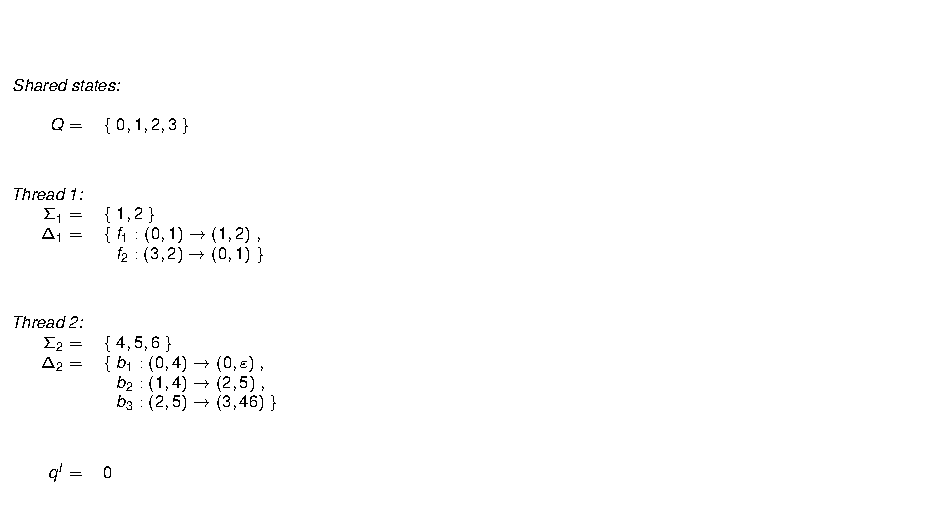
\includegraphics[width=.8\textwidth]{figures/cpds}
          \end{center}
        \end{column}
        \begin{column}{1\textwidth}
          % \documentclass[preview, landscape]{standalone}

% \usepackage{pgf}
% \usepackage{tikz}
% \usetikzlibrary{arrows,positioning}

% \newcommand{\config}[2]{\langle{#1\!\mid\!#2}\rangle} % compare typesetting: $q|x,y$ vs $q\mid x,y$ vs $q\!\mid\!x,y$
% \newcommand{\emptyword}  {\varepsilon}

% \usepackage{bbm}
% \usepackage{dsfont}
% \begin{document}
% \centerTwoOut{

% \begin{minipage}{.20\textwidth}
%   \[
%     \begin{array}{lll}
%       \pdsshareds & = & \{ \ 0, 1, 2, 3 \ \} \\[1em]

%       \alphabet_1 & = & \{ \ 1, 2 \ \} \\
%       \alphabet_2 & = & \{ \ 4, 5, 6 \ \}\\[1em]

%       \pdstranss_{1} & = &                  \{ \ f_1:     \threadstate 0 1  \pdstranssymbol \threadstate 1 2 \ , \\
%                      &   & \pos[r]{$f_2:$}{$\{ \ f_1:$} \ \threadstate 3 2  \pdstranssymbol \threadstate 0 1 \ \} \\[1em]
%       \pdstranss_{2} & = &                  \{ \ b_1:     \threadstate 0 4  \pdstranssymbol \threadstate 0 {\emptystack} \ , \\
%                      &   & \pos[r]{$b_2:$}{$\{ \ b_1:$} \ \threadstate 1 4  \pdstranssymbol \threadstate 2 5 \ , \\
%                      &   & \pos[r]{$b_3:$}{$\{ \ b_3:$} \ \threadstate 2 5  \pdstranssymbol \threadstate 3 {4 6} \ \} \\[1em]
%       \pdsinitstate  & = & 0
%     \end{array}
%   \]
%   % initial state:
%   % \[
%   %   \config 0 {1,4}
%   % \]
% \end{minipage}
% \hfill
\begin{minipage}{0.8\textwidth}
  \centering
  \resizebox{0.9\textwidth}{!}{
    \begin{tikzpicture}[->,>=stealth',shorten >=1pt,auto,node distance=2.0cm, semithick, 
      state/.style={minimum size=14pt,inner sep=-0.1pt,font=\small\rmfamily},
      round/.style = {rounded corners=1.5mm,dashed }, font=\sffamily]
      \tikzstyle{every state}=[minimum size=1mm]
      \tikzstyle{selected} = [draw,line width=5pt,-,gray!60]
      \begin{scope}[xshift=0cm,yshift=5cm]
        \draw[round] (-5.0,0.50) rectangle (3.0,-0.5);
        \node[] at (-4.6,-0.3) {$R_0$};
        \draw[round] (-5.1,0.55) rectangle (3.1,-2.0);
        \node[] at (-4.7,-1.8) {$R_1$};
        \draw[round] (-5.2,0.60) rectangle (3.2,-3.5);
        \node[] at (-4.8,-3.3) {$R_2$};
        \draw[round] (-5.3,0.65) rectangle (3.3,-5.0);
        \node[] at (-4.9,-4.8) {$R_3$};
        \draw[round] (-5.4,0.70) rectangle (3.4,-6.5);
        \node[] at (-5.0,-6.3) {$R_4$};
        \draw[round] (-5.5,0.75) rectangle (3.5,-8.0);
        \node[] at (-5.1,-7.8) {$R_5$};
        \draw[round] (-5.6,0.80) rectangle (3.6,-9.5);
        \node[] at (-5.2,-9.3) {$R_6$};
        \draw[round] (-5.7,0.85) rectangle (3.7,-10.0);
        \node[] at (-1.0,-9.8) {\bf ......};

        \draw[round] (6.0,0.50) rectangle (10.0,-0.5);
        \node[] at (6.3,-0.3) {$\visible[0]$};
        \draw[round] (5.9,0.55) rectangle (10.1,-2.0);
        \node[] at (6.2,-1.8) {$\visible[1]$};
        \draw[round] (5.8,0.60) rectangle (10.2,-3.5);
        \node[] at (6.1,-3.3) {$\visible[2]$};
        \draw[round,name=B] (5.7,0.65) rectangle (10.3,-5.0);
        \node[] at (6.0,-4.8) {$\visible[3]$};
        \draw[round] (5.6,0.70) rectangle (10.4,-6.5);
        \node[] at (5.9,-6.3) {$\visible[4]$};
        \draw[round] (5.5,0.75) rectangle (10.5,-8.0);
        \node[] at (5.8,-7.8) {$\visible[5]$};
        \draw[round] (5.4,0.80) rectangle (10.6,-9.5);
        \node[] at (5.7,-9.3) {$\visible[6]$};
        \draw[round] (5.3,0.85) rectangle (10.7,-10.0);
        \node[] at (8.1,-9.8) {\bf ......};

        \node[](1) at (8.0,0.0) {$\config 0 {1,4}$};
        \node[](2)[below =0.3cm of 1] {$\config 1 {2,4}$};
        \node[](3)[below =0.1cm of 2] {$\config 0 {1,\emptyword}$};
        \node[](4)[below =0.0cm of 3] {$\config 2 {2,5}$};
        \node[](5)[below left  = -0.5mm of 4] {$\config 3 {2,4}$};
        \node[](6)[below right = -0.5mm of 4] {$\config 1 {2,\emptyword}$};
        \node[color=blue](7) at (8.0,-5.8) {$\config 0 {1,6}$};
        \node[](8) [below = 0.7cm of 7] {$\config 1 {2,6}$};
        \draw[->, >=latex', shorten >=2pt, bend left=45, thick, dashed] 
        (2.9,0.3) to node[auto, swap] {$\mathcal T$}(6.1,0.3); 
        \draw[->, >=latex', shorten >=2pt, bend left=45, thick, dashed] 
        (3.0,-1.2) to node[auto, swap] {$\mathcal T$}(6.0,-1.2);
        \draw[->, >=latex', shorten >=2pt, bend left=45, thick, dashed] 
        (3.1,-2.7) to node[auto, swap] {$\mathcal T$}(5.9,-2.7);
        \draw[->, >=latex', shorten >=2pt, bend left=45, thick, dashed]  
        (3.3,-5.7) to node[auto, swap] {$\mathcal T$}(5.7,-5.7);
        \draw[->, >=latex', shorten >=2pt, bend left=45, thick, dashed] 
        (3.4,-7.2) to node[auto, swap] {$\mathcal T$}(5.6,-7.2);
        
        % k = 0
        \node[state] (014) {$\config 0 {1,4}$};
        % k = 1
        \node[state] (124) [below left of  = 014] {$\config 1 {2,4}$};
        \node[state] (01e) [below right of = 014] {$\config 0 {1,\emptyword}$};
        % k = 2
        \node[state] (225) [below = 1cm of 124] {$\config 2 {2,5}$};
        \node[state] (12e) [below = 1cm of 01e] {$\config 1 {2,\emptyword}$};
        \node[state] (3246) [left of  = 225] {$\config 3 {2,46}$};
        % k = 3
        \node[state,draw,color=red] (0146) [below = 1cm of 3246] {$\config 0 {1,46}$};
        \node[state,draw,color=red] (1246) [right of  = 0146] {$\config 1 {2,46}$};
        % k = 4
        \node[state,draw,color=blue] (016) [below = 1cm of 0146] {$\config 0 {1,6}$};
        \node[state] (2256) [right of  = 016] {$\config 2 {2,56}$};
        \node[state] (32466) [right = 1.2cm of 2256] {$\config 3 {2,466}$};
        % k = 5
        \node[state] (01466) [below = 1cm of 32466] {$\config 0 {1,466}$};
        \node[state] (12466) [left = 1.0cm of 01466] {$\config 1 {2,466}$};
        \node[state] (126) [below = 1cm of 016] {$\config 1 {2,6}$};
        % k = 6
        \node[state] (0166)  [below = 1cm of 01466] {$\config 0 {1,66}$};
        \node[state] (22566) [below = 1cm of 12466] {$\config 2 {2,566}$};
        \node[state] (324666) [below = 1cm of 126] {$\config 3 {2,4666}$};


        \draw [selected] (0146) -- (016);
        \path[]
        (014)  edge[left]     node {\scriptsize $f_1$} (124)
        (014)  edge[right]     node {\scriptsize $b_1$} (01e)
        (124)  edge[left]      node {\scriptsize $b_2$} (225)
        (01e)  edge[right]     node {\scriptsize $f_1$} (12e)
        (225)  edge[above]     node {\scriptsize $b_3$} (3246)
        (3246) edge[left]      node {\scriptsize $f_2$} (0146)
        (0146) edge[above]     node {\scriptsize $f_1$} (1246)
        (0146) edge[left]      node {\scriptsize $b_1$} (016)
        (1246) edge[right]     node {\scriptsize $b_2$} (2256)
        (2256) edge[above]     node {\scriptsize $b_3$} (32466)
        (32466)edge[right]     node {\scriptsize $f_2$} (01466)
        (01466)edge[above]     node {\scriptsize $f_1$} (12466)
        (016)  edge[left]      node {\scriptsize $f_1$} (126)
        (12466)edge[left]      node {\scriptsize $b_2$} (22566)
        (22566)edge[above]     node {\scriptsize $b_3$} (324666)
        (01466)edge[left]      node {\scriptsize $b_1$} (0166);
      \end{scope}
    \end{tikzpicture}}
\end{minipage}
% \end{document}

        \end{column}
      \end{columns}
    \end{block}
  }  
\end{frame}

\begin{frame}
  \frametitle{Stuttering Detection}
  \begin{block}{}
    \begin{columns}
      \begin{column}{0.49\textwidth}
        \begin{center}{\textbf{\textit{Stuttering}}}
          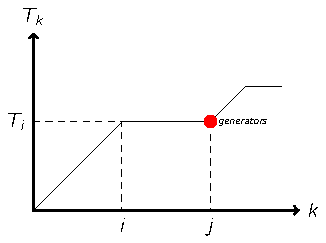
\includegraphics[width=1\textwidth]{figures/generator}
        \end{center}
      \end{column}
      \begin{column}{0.49\textwidth}
        \begin{center}{\textbf{\textit{Properties~[PLDI'18]}}}
          \vskip20pt
          \begin{enumerate}[\bhand]
          \item<1-> \emph{\small{generators are of special form\\ \alert{$\Rightarrow$} can be statically approximated}}
            \vskip25pt
          \item<2-> \emph{\small{all generators have been reached \\ \alert{$\Rightarrow$} OS converges}}
            \vskip25pt
          \item<3> \emph{\small{any overapproximation suffices}}
          \end{enumerate}
        \end{center}
      \end{column}
    \end{columns}
  \end{block}
\end{frame}

\begin{frame}
  \frametitle{Algorithm}
  \centering
  \resizebox{0.8\textwidth}{!}{
  \begin{tikzpicture}[%
    >=stealth,              % Nice arrows; your taste may be different
    start chain=going below,    % General flow is top-to-bottom
    node distance=6mm and 60mm, % Global setup of box spacing
    every join/.style={norm}]
    \tikzset{
      base/.style={draw, on chain, on grid, align=center, minimum height=4ex},
      proc/.style={base, rectangle, rounded corners},
      test/.style={base, diamond, aspect=2, rounded corners},
      term/.style={proc, draw=none},
      norm/.style={->, draw}
    }
    \node [term] (p0)
    {program $\pds$,
     property $\property$\\
     resource parameter $i:=0$
    };
    \node [proc, join] (Ok) {construct $\visible[i]$};
    \node [test, join] (violation) {$\visible[i]$ witnesses\\ a violation of $\property$?};
    \node [term, fill=red!60] (incorrect) {$\pds \not\models \property$};
    \node [proc, left=of Ok](kpp)  {$i:= i + 1$};
    \node [test, left=of violation, fill=blue!20] (converge) {$|\visible[i-1]| = |\visible[i]|$? };
    \node [test, left=of converge, fill=red!20] (stutter) {$\gens \subseteq \visible[i]$?};
    \node [term, fill=green!60] (correct) {$\pds \models \property$};

    \path (converge.north) to node [xshift=0.8em,yshift=0em] {\emph{no}} (kpp); 
    \draw [->] (converge.north) -- (kpp);
    \path (converge.west) to node [xshift=1.5em,yshift=2.5em] {\emph{yes}} (correct); 
    \draw [->] (converge.west) -- (stutter);
    \path (violation.west) to node [xshift=0em,yshift=0.5em] {\emph{no}} (converge); 
    \draw [->] (violation.west) -- (converge);
    \path (violation.south) to node [xshift=0.8em,yshift=0em] {\emph{yes}} (incorrect); 
    \draw [->] (violation.south) -- (incorrect);
    \path (stutter.south) to node [xshift=-13.8em,yshift=.9em] {\emph{yes}} (incorrect); 
    \draw [->] (stutter.south) -- (correct);
    \path (stutter.north) to node [xshift=-8.8em,yshift=8.2em] {\emph{no}} (incorrect);
    \draw [-] (stutter.north) -- (-12,-1.5);
    \draw [->] (-12,-1.5) -- (kpp.west);
    \draw [->,shorten <=1pt,shorten >=1pt] (kpp.east) -- (Ok);
  \end{tikzpicture}
}
\vskip2pt
$\gens := $\{\emph{reachable generators}\}
\end{frame}

\begin{frame}
  \frametitle{Example Revisited}
  \begin{block}{}
    \vspace{-4pt}
      $\scriptsize{\gens =  \{ \config 0 {1,\emptystack}, \config 0 {1,6} \}}$
    \begin{columns}
      \begin{column}{.95\textwidth}
          % \documentclass[preview, landscape]{standalone}

% \usepackage{pgf}
% \usepackage{tikz}
% \usetikzlibrary{arrows,positioning}

% \newcommand{\config}[2]{\langle{#1\!\mid\!#2}\rangle} % compare typesetting: $q|x,y$ vs $q\mid x,y$ vs $q\!\mid\!x,y$
% \newcommand{\emptyword}  {\varepsilon}

% \usepackage{bbm}
% \usepackage{dsfont}
% \begin{document}
% \centerTwoOut{

% \begin{minipage}{.20\textwidth}
%   \[
%     \begin{array}{lll}
%       \pdsshareds & = & \{ \ 0, 1, 2, 3 \ \} \\[1em]

%       \alphabet_1 & = & \{ \ 1, 2 \ \} \\
%       \alphabet_2 & = & \{ \ 4, 5, 6 \ \}\\[1em]

%       \pdstranss_{1} & = &                  \{ \ f_1:     \threadstate 0 1  \pdstranssymbol \threadstate 1 2 \ , \\
%                      &   & \pos[r]{$f_2:$}{$\{ \ f_1:$} \ \threadstate 3 2  \pdstranssymbol \threadstate 0 1 \ \} \\[1em]
%       \pdstranss_{2} & = &                  \{ \ b_1:     \threadstate 0 4  \pdstranssymbol \threadstate 0 {\emptystack} \ , \\
%                      &   & \pos[r]{$b_2:$}{$\{ \ b_1:$} \ \threadstate 1 4  \pdstranssymbol \threadstate 2 5 \ , \\
%                      &   & \pos[r]{$b_3:$}{$\{ \ b_3:$} \ \threadstate 2 5  \pdstranssymbol \threadstate 3 {4 6} \ \} \\[1em]
%       \pdsinitstate  & = & 0
%     \end{array}
%   \]
%   % initial state:
%   % \[
%   %   \config 0 {1,4}
%   % \]
% \end{minipage}
% \hfill
\begin{minipage}{1\textwidth}
  \centering
  \resizebox{.90\textwidth}{!}{
    \begin{tikzpicture}[->,>=stealth',shorten >=1pt,auto,node distance=2.0cm, semithick, 
      state/.style={minimum size=14pt,inner sep=-0.1pt,font=\small\rmfamily},
      round/.style = {rounded corners=1.5mm,dashed }, font=\sffamily]
      \tikzstyle{every state}=[minimum size=1mm]
      \tikzstyle{selected} = [draw,line width=5pt,-,gray!60]
      \begin{scope}[xshift=0cm,yshift=5cm]
        \draw[round] (-5.0,0.50) rectangle (3.0,-0.5);
        \node[] at (-4.6,-0.3) {$R_0$};
        \draw[round] (-5.1,0.55) rectangle (3.1,-2.0);
        \node[] at (-4.7,-1.8) {$R_1$};
        \draw[round] (-5.2,0.60) rectangle (3.2,-3.5);
        \node[] at (-4.8,-3.3) {$R_2$};
        \draw[round] (-5.3,0.65) rectangle (3.3,-5.0);
        \node[] at (-4.9,-4.8) {$R_3$};
        \draw[round] (-5.4,0.70) rectangle (3.4,-6.5);
        \node[] at (-5.0,-6.3) {$R_4$};
        \draw[round] (-5.5,0.75) rectangle (3.5,-8.0);
        \node[] at (-5.1,-7.8) {$R_5$};
        \draw[round] (-5.6,0.80) rectangle (3.6,-9.5);
        \node[] at (-5.2,-9.3) {$R_6$};
        \draw[round] (-5.7,0.85) rectangle (3.7,-10.0);
        \node[] at (-1.0,-9.8) {\bf ......};

        \draw[round] (6.0,0.50) rectangle (10.0,-0.5);
        \node[] at (6.3,-0.3) {$\visible[0]$};
        \draw[round] (5.9,0.55) rectangle (10.1,-2.0);
        \node[] at (6.2,-1.8) {$\visible[1]$};
        \draw[round] (5.8,0.60) rectangle (10.2,-3.5);
        \node[] at (6.1,-3.3) {$\visible[2]$};
        \draw[round,name=B] (5.7,0.65) rectangle (10.3,-5.0);
        \node[] at (6.0,-4.8) {$\visible[3]$};
        \draw[round] (5.6,0.70) rectangle (10.4,-6.5);
        \node[] at (5.9,-6.3) {$\visible[4]$};
        \draw[round] (5.5,0.75) rectangle (10.5,-8.0);
        \node[] at (5.8,-7.8) {$\visible[5]$};
        \draw[round] (5.4,0.80) rectangle (10.6,-9.5);
        \node[] at (5.7,-9.3) {$\visible[6]$};
        \draw[round] (5.3,0.85) rectangle (10.7,-10.0);
        \node[] at (8.1,-9.8) {\bf ......};

        \node[](1) at (8.0,0.0) {$\config 0 {1,4}$};
        \node[](2)[below =0.3cm of 1] {$\config 1 {2,4}$};
        \node[](3)[below =0.1cm of 2] {$\config 0 {1,\emptyword}$};
        \node[](4)[below =0.0cm of 3] {$\config 2 {2,5}$};
        \node[](5)[below left  = -0.5mm of 4] {$\config 3 {2,4}$};
        \node[](6)[below right = -0.5mm of 4] {$\config 1 {2,\emptyword}$};
        \node[](7) at (8.0,-5.8) {$\config 0 {1,6}$};
        \node[](8) [below = 0.7cm of 7] {$\config 1 {2,6}$};
        \draw[->, >=latex', shorten >=2pt, bend left=45, thick, dashed] 
        (2.9,0.3) to node[auto, swap] {$\mathcal T$}(6.1,0.3); 
        \draw[->, >=latex', shorten >=2pt, bend left=45, thick, dashed] 
        (3.0,-1.2) to node[auto, swap] {$\mathcal T$}(6.0,-1.2);
        \draw[->, >=latex', shorten >=2pt, bend left=45, thick, dashed] 
        (3.1,-2.7) to node[auto, swap] {$\mathcal T$}(5.9,-2.7);
        \draw[->, >=latex', shorten >=2pt, bend left=45, thick, dashed]  
        (3.3,-5.7) to node[auto, swap] {$\mathcal T$}(5.7,-5.7);
        \draw[->, >=latex', shorten >=2pt, bend left=45, thick, dashed] 
        (3.4,-7.2) to node[auto, swap] {$\mathcal T$}(5.6,-7.2);
        
        % k = 0
        \node[state] (014) {$\config 0 {1,4}$};
        % k = 1
        \node[state] (124) [below left of  = 014] {$\config 1 {2,4}$};
        \node[state] (01e) [below right of = 014] {$\config 0 {1,\emptyword}$};
        % k = 2
        \node[state] (225) [below = 1cm of 124] {$\config 2 {2,5}$};
        \node[state] (12e) [below = 1cm of 01e] {$\config 1 {2,\emptyword}$};
        \node[state] (3246) [left of  = 225] {$\config 3 {2,46}$};
        % k = 3
        \node[state,draw,color=red] (0146) [below = 1cm of 3246] {$\config 0 {1,46}$};
        \node[state,draw,color=red] (1246) [right of  = 0146] {$\config 1 {2,46}$};
        % k = 4
        \node[state] (016) [below = 1cm of 0146] {$\config 0 {1,6}$};
        \node[state] (2256) [right of  = 016] {$\config 2 {2,56}$};
        \node[state] (32466) [right = 1.2cm of 2256] {$\config 3 {2,466}$};
        % k = 5
        \node[state] (01466) [below = 1cm of 32466] {$\config 0 {1,466}$};
        \node[state] (12466) [left = 1.0cm of 01466] {$\config 1 {2,466}$};
        \node[state] (126) [below = 1cm of 016] {$\config 1 {2,6}$};
        % k = 6
        \node[state] (0166)  [below = 1cm of 01466] {$\config 0 {1,66}$};
        \node[state] (22566) [below = 1cm of 12466] {$\config 2 {2,566}$};
        \node[state] (324666) [below = 1cm of 126] {$\config 3 {2,4666}$};


        \draw [selected] (0146) -- (016);
        \path[]
        (014)  edge[left]     node {\scriptsize $f_1$} (124)
        (014)  edge[right]     node {\scriptsize $b_1$} (01e)
        (124)  edge[left]      node {\scriptsize $b_2$} (225)
        (01e)  edge[right]     node {\scriptsize $f_1$} (12e)
        (225)  edge[above]     node {\scriptsize $b_3$} (3246)
        (3246) edge[left]      node {\scriptsize $f_2$} (0146)
        (0146) edge[above]     node {\scriptsize $f_1$} (1246)
        (0146) edge[left]      node {\scriptsize $b_1$} (016)
        (1246) edge[right]     node {\scriptsize $b_2$} (2256)
        (2256) edge[above]     node {\scriptsize $b_3$} (32466)
        (32466)edge[right]     node {\scriptsize $f_2$} (01466)
        (01466)edge[above]     node {\scriptsize $f_1$} (12466)
        (016)  edge[left]      node {\scriptsize $f_1$} (126)
        (12466)edge[left]      node {\scriptsize $b_2$} (22566)
        (22566)edge[above]     node {\scriptsize $b_3$} (324666)
        (01466)edge[left]      node {\scriptsize $b_1$} (0166);

        \node[circle, draw, color=red, inner sep=2pt, minimum size=1pt] (s1) [below = 1cm of 6] {};
        \node[circle, draw, color=red,inner sep=3pt,minimum size=1pt](s2) [above right = 0.5cm of s1] {};
        \node[circle, draw, color=red,inner sep=4pt,minimum size=1pt](s3) [above right = 0.5cm of s2] {};
        \node[circle, draw, color=red,inner sep=5pt,minimum size=1pt](s4) [above right = 0.5cm of s3] {};
        \node[cloud,draw,color=red] (stuttering) [above right = 0.5 of s4] {\emph{stuttering}};

        \node[circle, draw, color=blue, inner sep=2pt, minimum size=1pt] (c1) [below right = 1.5cm of 8] {};
        \node[circle, draw, color=blue,inner sep=3pt,minimum size=1pt](c2) [above right = 0.5cm of c1] {};
        \node[circle, draw, color=blue,inner sep=4pt,minimum size=1pt](c3) [above right = 0.5cm of c2] {};
        \node[circle, draw, color=blue,inner sep=5pt,minimum size=1pt](c4) [above right = 0.5cm of c3] {};
        
        \node[cloud,draw,color=blue] (converge) [above right = 0.5 of c4] {\emph{converge}};
      \end{scope}
    \end{tikzpicture}}
\end{minipage}
% \end{document}

      \end{column}
    \end{columns}
  \end{block}
\end{frame}

\begin{frame}
  \frametitle{Empirical Evaluation}
  \only<1>{
    \begin{block}{\emph{Performance}}
      \vskip6pt
      % \includegraphics[width=\textwidth]{figures/exp-table}
      \centering
\renewcommand{\arraystretch}{1.3}
\resizebox{6.8cm}{!}{
  \noindent
  \begin{tabular}{@{}lcc@{}c@{}lr@{}}
    \hline
    \multirow{2}{*}{ID/Program} & \multicolumn{2}{c}{Prog. Features} & \multirow{2}{*}{\ \ } & \multicolumn{2}{c}{$\family{T_k}$} \\
    \cline{2-3}\cline{5-6}\noalign{\smallskip}
    & \multicolumn{1}{@{}c@{}}{~$\mathit{Thread}$~} 
    & \multicolumn{1}{r}{$\mathit{Safe}?$} 
    &                                                                                 
    & \multicolumn{1}{l}{$k_{\mathit{max}}$~}
    & \multicolumn{1}{r@{}}{~$Time~(sec.)$~}\\   
    \hline
    \multirow{3}{*}{\textsc{1/Bluetooth-1\hspace{1mm}}}
                                              & $\recur 1 + \recur 1$ & $\No$ & & 6~(4) &0.26 \\
                                              & $\recur 1 + \recur 2$ & $\No$ & & 6~(3) &2.32 \\
                                              & $\recur 2 + \recur 1$ & $\No$ & & 7~(4) &12.76 \\
    \hline
    \multirow{3}{*}{\textsc{2/Bluetooth-2}}   & $\recur 1 + \recur 1$ & $\No$ & & 6~(4) &0.53 \\
                                              & $\recur 1 + \recur 2$ & $\No$ & & 6~(3) &4.39 \\
                                              & $\recur 2 + \recur 1$ & $\No$ & & 7~(4) &14.21\\
    \hline
    \multirow{3}{*}{\textsc{3/Bluetooth-3}}   & $\recur 1 + \recur 1$ & $\Yes$ & & 6 &0.47 \\
                                              & $\recur 1 + \recur 2$ & $\Yes$ & & 6 &4.71 \\
                                              & $\recur 2 + \recur 1$ & $\Yes$ & & 7 &14.46 \\
     & & & & & \\
    \hline
  \end{tabular}}
\hfill
\resizebox{6.8cm}{!}{
  \noindent 
  \begin{tabular}{@{}llcc@{}c@{}r@{}crrr@{}}
    \hline
    \multirow{2}{*}{ID/Program} & \multicolumn{2}{c}{Prog. Features} & \multirow{2}{*}{\ \ } & \multicolumn{2}{c}{$\family{T_k}$} \\
    \cline{2-3}\cline{5-6}\noalign{\smallskip}
    & \multicolumn{1}{@{}c@{}}{~$\mathit{Thread}$~} 
    & \multicolumn{1}{r}{$\mathit{Safe}?$} 
    &                                                                                 
    & \multicolumn{1}{l}{$k_{\mathit{max}}$~}
    & \multicolumn{1}{r@{}}{~$Time~(sec.)$~} \\      
    \hline
    \multirow{3}{*}{\textsc{4/BST-Insert}}   & $\recur 1 + \recur 1$   & $\Yes$ & & 2 & 1.17 \\
                                             & $\recur 2 + \recur 1$   & $\Yes$ & & 3 & 15.84 \\
                                             & $\recur 2 + \recur 2$   & $\Yes$ & & 4 & 45.21 \\
    \hline
    \multirow{1}{*}{\textsc{5/FileCrawler}} & $\nonrecur 1+\recur 2$  & $\Yes$ & & 6 & 0.03   \\
    \hline
    \multirow{1}{*}{\textsc{6/K-Induction}} & $\recur 1+\recur 1$     & $\Yes$ & & 3 & 0.23  \\
    \hline
    \multirow{1}{*}{\textsc{7/Proc-2}}      & $\recur 2+\nonrecur 2$  & $\Yes$ & & 3 & 0.52  \\
    \hline
    \multirow{2}{*}{\textsc{8/Stefan-1}}  & $\recur 2$  & $\Yes$ & & $2$ & $1.01$   \\
                                          & $\recur 4$  & $\Yes$ & & $4$ & $16.36$  \\
                                          & $\recur 8$  & $-$    & & $\atl 8$    & $-$  \\
    \hline
    \multirow{1}{*}{\textsc{9/Dekker}}    & $\nonrecur 2$ & $\Yes$ & & 6 & 0.21  \\
    \hline
  \end{tabular}}                               
    \end{block}}
  % \only<2>{
  %   \begin{block}{vs \JMoped~[SPIN'08]}
  %     \vskip2pt
  %     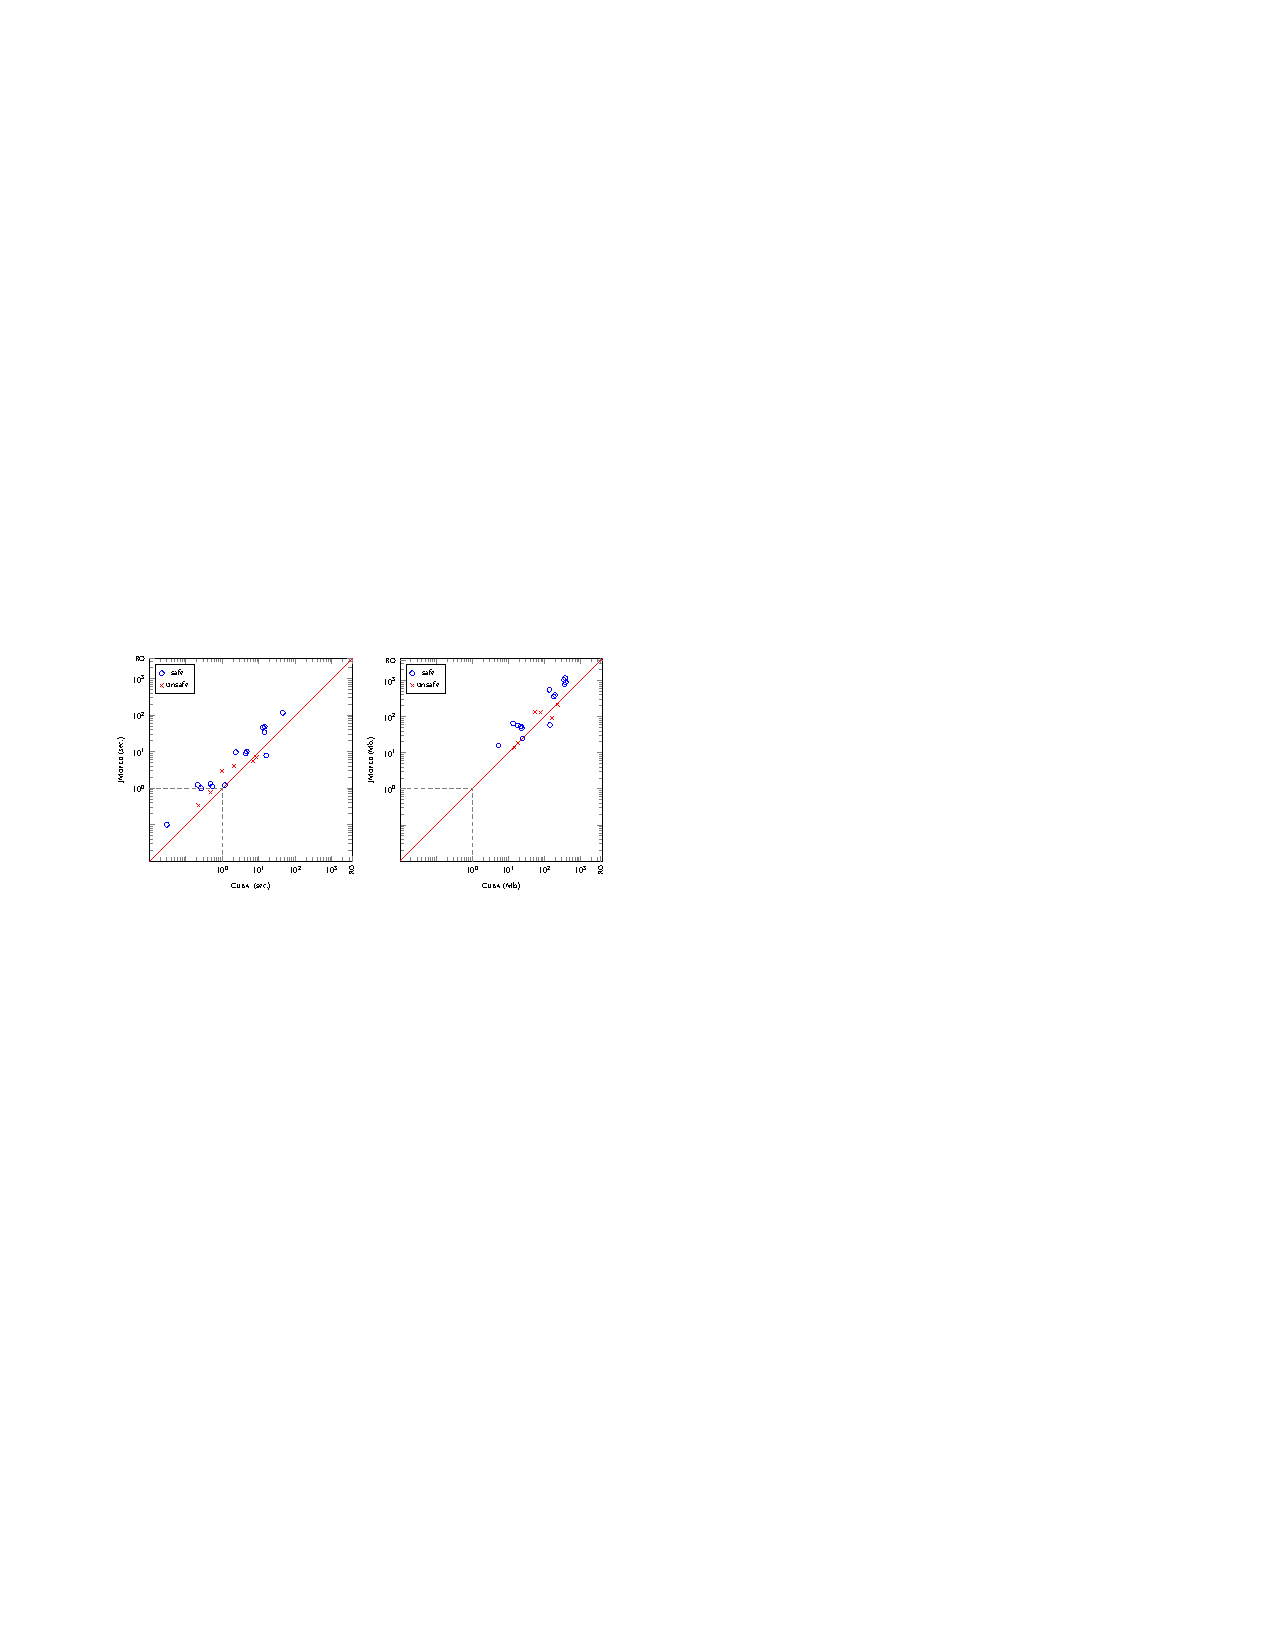
\includegraphics[width=\textwidth]{figures/exp-comp}
  %   \end{block}
  % }
\end{frame}

\section{Proposed Work: Applications and Beyond}
\begin{frame}
  \frametitle{Queue-Parameterized Analysis}
  \only<1>{
  \begin{block}{\emph{Target is ...}}
    \centering
    \vskip2pt
    \emph{message-passing programs.}
  \end{block}
  \begin{block}{\emph{Resource is ...}}
    \centering
    \vskip2pt
    \emph{the size of \alert{message queues}.}
  \end{block}
  \begin{block}{\emph{Observation is ...}}
    \centering
    \vskip2pt
    \emph{the set of \alert{reachable} program states w.r.t. the size of queue within $k$.}
  \end{block}
  \begin{block}{\emph{Analysis is ...}}
    \centering
    \vskip2pt
    \emph{to check the reachability of \alert{bad} states.}
  \end{block}}
\end{frame}

\begin{frame}
  \frametitle{Motivation}
  % \only<1>{
  %   \begin{block}{\emph{Why message passing programs? Because ...}}
  %     \vskip4pt
  %     % \begin{center}
  %       {\bhand} \emph{they are widely implemented in distributed systems, and }\\
  %       {\bhand} \emph{ensuring their safety is desirable.}
  %     % \end{center}
  %   \end{block}}   
  \only<1>{
    \begin{block}{\emph{Why message queues? Because they are ...}}
      \vskip4pt
      \begin{enumerate}[{\bhand}]
      \item \emph{a key \alert{synchronization} mechanism;}
      \item \emph{a key reason to generate \alert{infinite} state space;}
      \item \emph{a key reason to cause \alert{undecidability} of reachabililty analysis.}
      \end{enumerate}
    \end{block}
    \begin{block}{\emph{Bounding message queues gives us ...}}
      \vskip4pt
      \begin{enumerate}[{\bhand}]
      \item \emph{an easier problem:}\\
        % \alert{$\Rightarrow$} \emph{$\reached[k]$ is \alert{finite} and \alert{computable}.}
        % \alert{$\Rightarrow$}
        \emph{\scriptsize{Queue-\alert{bounded} reachability analysis of message passing programs is often \alert{decidable}}.}
      \end{enumerate}
    \end{block}}
\end{frame}

\begin{frame}
  \frametitle{Our Plan: Theory Investigation}
  \only<1>{
    \begin{block}{\emph{Step 1: Define observation sequences}}
      \vskip4pt
      \begin{enumerate}[{\bhand}]        
      \item \emph{$\OS := \reached[0], \reached[1],\reached[2], \ldots$.} \\
       \alert{$\Rightarrow$} \emph{\scriptsize $\reached[k]$ := the set of reachable states when \alert{message queues} are bounded by $k$.}
      \item \emph{Projecting $\reached[k]$ to a smaller finite domain ...}
      \end{enumerate}
    \end{block}
  } 
  \only<2>{
    \begin{block}{\emph{Step 2: Convergence detection}}
      \vskip4pt
      \begin{enumerate}[{\bhand}]
      \item \emph{Message queues are quite different from contexts.}\\
        \alert{$\Rightarrow$} \emph{How to proceed?}
      \end{enumerate}
    \end{block}
  }
\end{frame}

\begin{frame}
  \frametitle{Our Plan: Empirical Evaluation}
  \only<1>{
    \begin{block}{\emph{We will ...}}
      \vskip4pt
      \begin{enumerate}[{\bhand}]
      \item \emph{evaluate our approach on an extensive collection of P programs~[PLDI'13].}
      \end{enumerate}
      % \alert{$\Rightarrow$} \emph{Access-bounded reachability analysis of CPDS is \alert{decidable}.}
    \end{block}
  }
\end{frame}

\section{Conclusion and Schedule}
\begin{frame}
  \frametitle{Conclusion}
  \only<1>{
    \begin{block}{\emph{We target ...}}
      \vskip2pt
      \emph{resource-parameterized programs.}
      \centering
    \end{block}
    \begin{block}{\emph{We propose ...}}
      \vskip2pt
      \emph{a uniform paradigm of observation sequences.}
      \centering
    \end{block}}
  \only<2>{
    \begin{block}{\emph{The paradigm ...}}
      \vskip2pt
      \centering
      \resizebox{0.5\textwidth}{!}{
        %%% Local Variables:
%%% mode: latex
%%% TeX-master: t
%%% End:

  \begin{tikzpicture}[%
    >=stealth,              % Nice arrows; your taste may be different
    start chain=going below,    % General flow is top-to-bottom
    node distance=6mm and 60mm, % Global setup of box spacing
    every join/.style={norm}]
    \tikzset{
      base/.style={draw, on chain, on grid, align=center, minimum height=4ex},
      proc/.style={base, rectangle, rounded corners},
      test/.style={base, diamond, aspect=2, rounded corners},
      term/.style={proc, draw=none},
      norm/.style={->, draw}
    }
    \node [term] (p0)
    {program $\pds$,
      property $\property$\\
      resource parameter $i:=0$
    };
    \node [proc, join] (Ok) {construct $\observation[i]$};
    \node [test, join] (violation) {$\observation[i]$ witnesses\\ a violation of $\property$?};
    \node [term, fill=red!60] (incorrect) {$\pds \not\models \property$};
    \node [proc, left=of Ok](kpp)  {$i := i + 1$};
    \node [test] (converge) {sequence {\scriptsize $\OS$}\\ \alert{converges} at $i$?};
    \node [term, fill=green!60] (correct) {$\pds \models \property$};

    \path (converge.north) to node [xshift=0.8em,yshift=0em] {\emph{no}} (kpp); 
    \draw [->] (converge.north) -- (kpp);
    \path (converge.south) to node [xshift=1em,yshift=0em] {\emph{yes}} (correct); 
    \draw [->] (converge.south) -- (correct);
    \path (violation.west) to node [xshift=0em,yshift=0.5em] {\emph{no}} (converge); 
    \draw [->] (violation.west) -- (converge);
    \path (violation.south) to node [xshift=1em,yshift=0em] {\emph{yes}} (incorrect); 
    \draw [->] (violation.south) -- (incorrect);
    \draw [->,shorten <=1pt,shorten >=1pt] (kpp.east) -- (Ok);
  \end{tikzpicture}
      }
      \vskip15pt
      \emph{\textbf{can lift the bug-finding technique to resource-unbounded analysis.}}
    \end{block}}

  \only<3>{
    \begin{block}{\emph{We target ..}}
      \vskip2pt
      \emph{resource-parameterized programs.}
      \centering
    \end{block}
    \begin{block}{\emph{We proposed ...}}
      \vskip2pt
      \emph{a uniform paradigm of observation sequences.}
      \centering
    \end{block}
    \begin{block}{\emph{The paradigm can lift ...}}
      \vskip2pt
      \emph{the bug-finding technique to resource-unbounded analysis.}
      \centering
    \end{block}
    \begin{block}{\emph{We applied it ...}}
      \vskip2pt
      \emph{to context-unbounded analysis.}
      \centering
    \end{block}
    \begin{block}{\emph{We plan to ...}}
      \vskip2pt
      \emph{extend it to more applications.}
      \centering
    \end{block}}
\end{frame}

\begin{frame}
  \frametitle{Schedule}
  \only<1>{ 
    \begin{block}{}
      \begin{center}
      \resizebox{15cm}{!}{
        \begin{tabular}{rcl}
          October 2018 & \hspace{5pt} & Proposal\\
          October 2018 -- February 2019 & & Queue-parameterized analysis\\                                 
          February 2019 -- May 2019    & & More applications\\ %Shared-Memory Access-Parameterized Analysis\\                               
          May 2019 -- July 2019 & & Improving the scalability of our tools; writing dissertation \\
          August 2019 && Defense                                 
        \end{tabular}
      }
      \end{center}
    \end{block}
  }
\end{frame}

\subsection*{Thank You}
\begin{frame}
  \frametitle{Thank You}
  \begin{block}{References}
    \vskip4pt
      \small{
      \bibliographystyle{ieee}
      \renewcommand{\section}[2]{\vskip 0.05em}
      \begin{thebibliography}{1}\itemsep=-0.01em \setlength{\baselineskip}{0.4em}
      \bibitem{R00} Ramalingam, G.: ``Context-sensitive synchronization-sensitive analysis is undecidable.'' In: ACM
        Trans. Program. Lang. Syst. (2000)

        \bibitem{TACAS05} Qadeer, S., Rehof, J.: ``Context-bounded model checking of concurrent software.'' In: TACAS. (2005)

      \bibitem{ASPLOS08} Lu, S., Park, S., Seo, E., Zhou, Y.: ``Learning from mistakes: a comprehensive study on real
          world concurrency bug characteristics.'' In: ASPLOS. (2008)

       \bibitem{PLDI13} Desai, A., Gupta, V., Jackson, E., Qadeer, S., Rajamani, S., Zufferey, D.: ``P: Safe asynchronous event-driven programming.'' In: PLDI. (2013)

      \bibitem{PLDI18} Liu, P., Wahl, T.: ``CUBA: Interprocedural context-unbounded analysis of concurrent programs.''
        In: PLDI. (2018)
      \end{thebibliography}}
  \end{block}
\end{frame}

%==============================Ending main Section=============================%
%==============================Backup slides=============================%
% \peizun{
\begin{frame}
  \frametitle{Empirical Evaluation}
  % \only<1>{
  %   \begin{block}{Performance}
  %     \vskip2pt
  %     \includegraphics[width=\textwidth]{figures/exp-table}
  %   \end{block}}
  \only<1>{
    \begin{block}{vs \JMoped~[SPIN'08]}
      \vskip2pt
      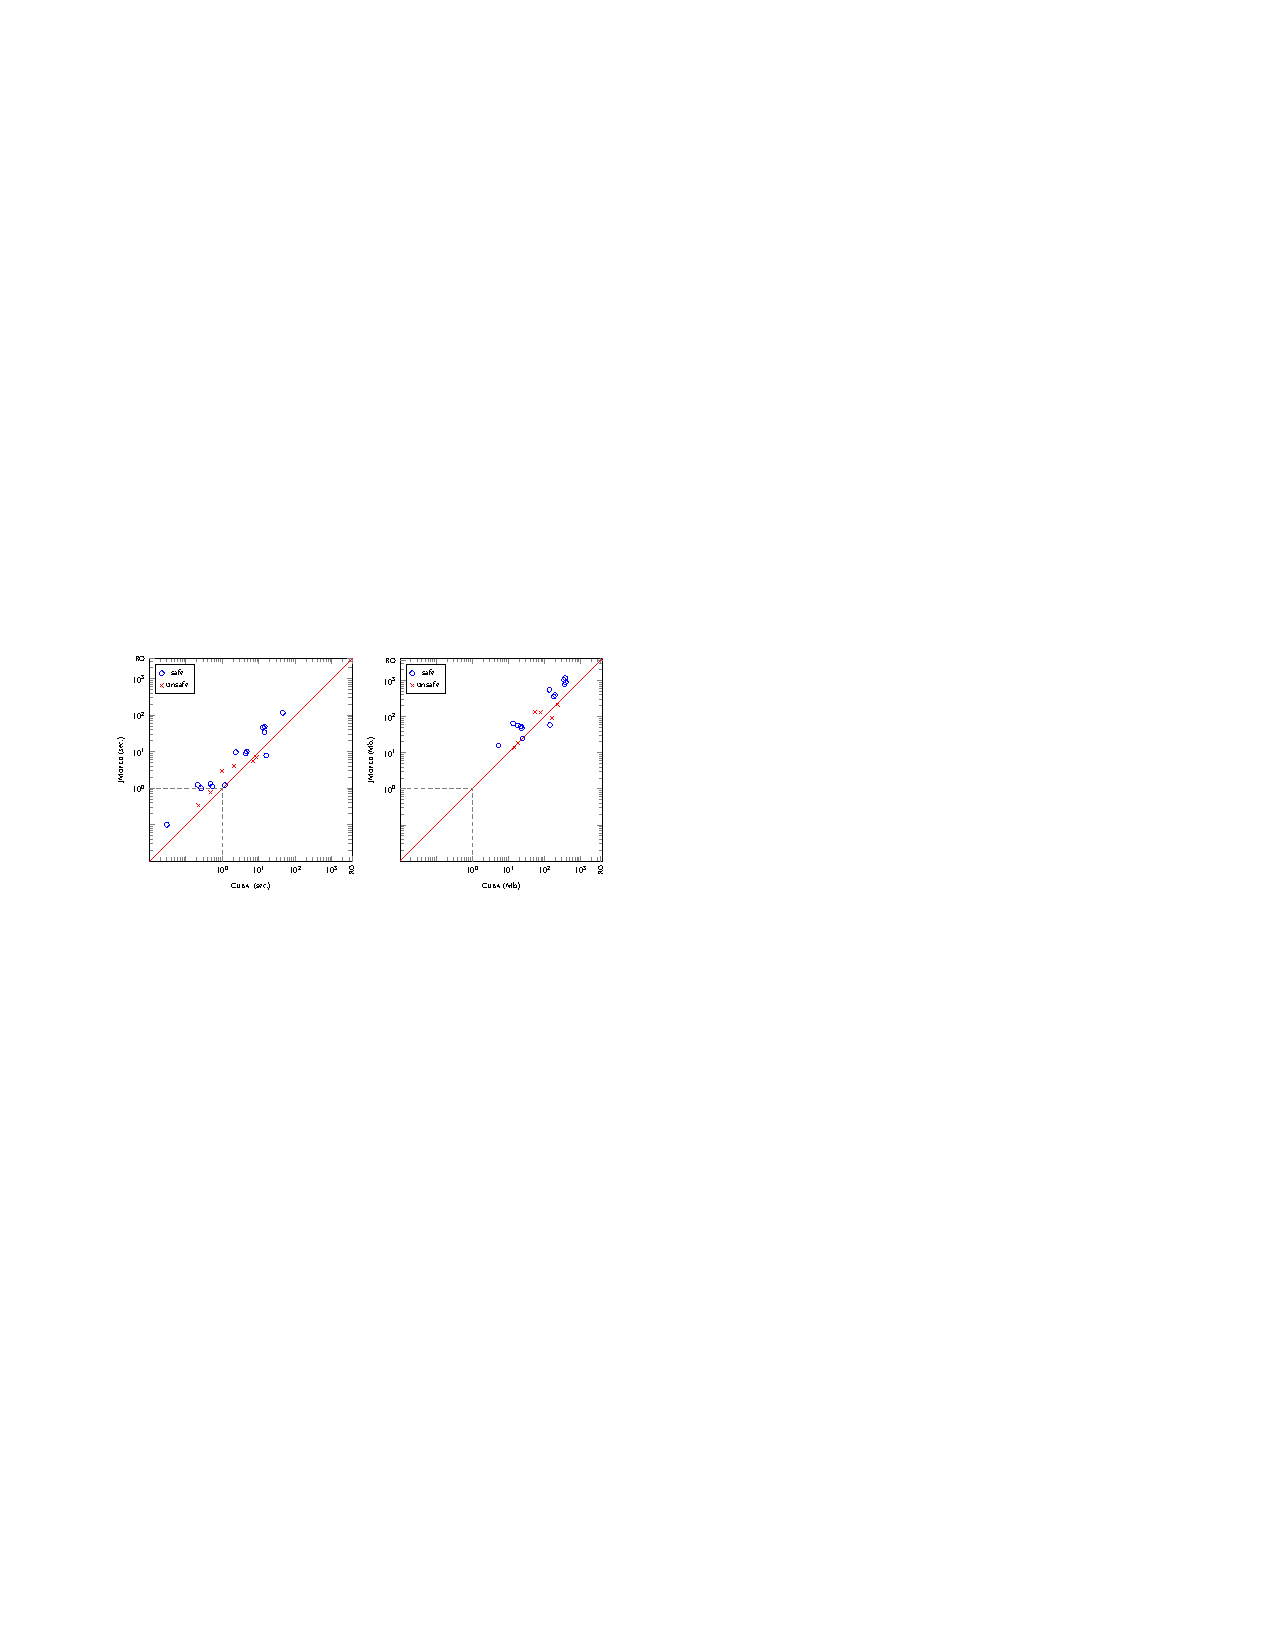
\includegraphics[width=\textwidth]{figures/exp-comp}
    \end{block}
  }
\end{frame}

\begin{frame}
  \frametitle{Shared-Memory Access-Parameterized Analysis}
  \only<1>{
  \begin{block}{\emph{Target is ...}}
    \vskip2pt
    \centering
    \emph{shared-memory multi-threaded programs.}
  \end{block}
  \begin{block}{\emph{Resource is ...}}
    \vskip2pt
    \centering
    \emph{the number of shared-memory accesses.}
  \end{block}
  \begin{block}{\emph{Observation is ...}}
    \vskip2pt
    \centering
    \emph{the set of \alert{reachable} program states w.r.t. $k$ accesses.}
  \end{block}
  \begin{block}{\emph{Verification is ...}}
    \vskip2pt
    \centering
    \emph{reduced to the reachability of \alert{bad} states.}
  \end{block}}
\end{frame}

\begin{frame}
  \frametitle{Motivation}
  \only<1>{
    \begin{block}{\emph{Why shared-memory accesses?}}
    \end{block}}   
  \only<2>{
    \begin{block}{\emph{Reason 1}}
      \vskip4pt
      \begin{enumerate}[{\bhand}]
      \item \emph{Improper shared-memory accesses are a \alert{root cause}
          of concurrency bugs}
      \end{enumerate}      
        \alert{$\Rightarrow$} \emph{\small{E.g., race condition, data race etc. }}
    \end{block}
    \begin{block}{\emph{Unfortunately,}}
      \vskip4pt
      \begin{enumerate}[{\bhand}]
      \item \emph{Analysis with \emph{unbounded} accesses is challenging}
      \end{enumerate}
    \end{block}} 
  \only<3>{\begin{block}{\emph{Reason 2}}
      \vskip4pt
      \begin{enumerate}[{\bhand}]
      \item \emph{Have an easier problem if bounding the number of accesses}
      \end{enumerate}
      \alert{$\Rightarrow$} \emph{\small{Access-bounded reachability analysis of CPDS is \alert{decidable} [proved]}}\\
      \alert{$\Rightarrow$} \emph{\small{Many bugs can be exposed with \alert{few} shared-memory accesses~[ASPLOS'08]}}
    \end{block}
    % \begin{block}{\emph{But, uncertainty still exists ...}}
    %   \vskip4pt
    %   \begin{enumerate}[{\bhand}]
    %   \item \emph{Eliminating \alert{uncertainty} is desirable}
    %   \end{enumerate}
    % \end{block}
  }
\end{frame}

\begin{frame}
  \frametitle{Our Plan: Theory Investigation}
  \only<1>{
    \begin{block}{\emph{Step 1: Define observation sequences}}
      \vskip4pt
      \begin{enumerate}[{\bhand}]        
      \item \emph{$\OS := \reached[0], \reached[1],\reached[2], \ldots$.} \\
        \alert{$\Rightarrow$} \emph{$\reached[k]$ = the set of states reachable within $k$ accesses.}
      \item \emph{Projecting $\reached[k]$ to a finite domain ...}
      \end{enumerate}
    \end{block}
  } 
  \only<2>{
    \begin{block}{\emph{Step 2: Convergence detection}}
      \vskip4pt
      \begin{enumerate}[{\bhand}]
      \item \emph{Based on similar convergence detection used in CUBA, and ...}
      \end{enumerate}
    \end{block}
  }
  \only<3>{
    \begin{block}{\emph{Step 3: A decidable subclass}}
      \vskip4pt
      \begin{enumerate}[{\bhand}]
      \item \emph{We will define a decidable subclass of shared-memory multi-threaded programs.}\\
        \alert{$\Rightarrow$} \emph{What does this mean?}
      \end{enumerate}
    \end{block}}
\end{frame}

\begin{frame}
  \frametitle{Our Plan: Empirical Evaluation}
  \only<1>{
    \begin{block}{\emph{We will }}
      \vskip4pt
      \begin{enumerate}[{\bhand}]
      \item \emph{evaluate our approach on an extensive collection of shared-memory multi-threaded programs.}
      \end{enumerate}
      % \alert{$\Rightarrow$} \emph{Access-bounded reachability analysis of CPDS is \alert{decidable}.}
    \end{block}
  }
\end{frame}

\peizun{
\begin{frame}
  \frametitle{Questions [for us only]}
  \begin{block}{}
    1. can you provide a uniform tool?\\

    2. can you provide a guide to users, e.g. how to define k, Ok,  etc.? \\

    3. So you have basically presented one solution to one problem (PLDI 2018).
    How will you approach the othe problems (access-param., queue-param., etc)
    -- all in the same way? does the PLDI approach generalize?
  \end{block}
\end{frame}}

\end{document}
